
\documentclass[a4paper, 12pt, twoside]{book}

\usepackage{fontspec} % package spécifique à XeLaTeX
\usepackage[english, french]{babel} %package spécificité des langues + mention de langue voulue
\usepackage{minted} % paquet pour créer un environnement de code coloré
\usepackage{wrapfig} % paquet pour images
\usepackage{caption}
\usepackage{subcaption}
\usepackage[xetex]{graphicx} % paquet pour insérer des images
\usepackage{longtable}
\usepackage{lscape}
\usepackage{pdflscape}
\usepackage[dvipsnames]{xcolor} % pour les couleurs
\usepackage{imakeidx} % doit se trouver avant hypperef pour éviter des pb de compilations. Permet de créer les index
\makeindex
\usepackage[xetex]{hyperref}
\usepackage{listings} % package pour lstlisting : portion de codes avec des numéros de lignes

\lstset{
	language=python, % définition du langage
	basicstyle=\scriptsize\ttfamily, % petite taille, police de console
	stringstyle=\color{Mahogany}, % chaîne de caractères
	backgroundcolor=\color{white}, % fond
	commentstyle=\color{Melon}\textit, % commentaires
	numberstyle=\tiny\color{darkgray}, % numéro de ligne
	rulecolor=\color{lightgray}, % bordure
	keywordstyle=\color{OrangeRed}\textbf, % opérateurs logiques etc
	literate=
	{0}{{{\ProcessDigit{0}}}}1
	{1}{{{\ProcessDigit{1}}}}1
	{2}{{{\ProcessDigit{2}}}}1
	{3}{{{\ProcessDigit{3}}}}1
	{4}{{{\ProcessDigit{4}}}}1
	{5}{{{\ProcessDigit{5}}}}1
	{6}{{{\ProcessDigit{6}}}}1
	{7}{{{\ProcessDigit{7}}}}1
	{8}{{{\ProcessDigit{8}}}}1
	{9}{{{\ProcessDigit{9}}}}1
	{<=}{{\(\leq\)}}1,
	morestring=[b]",
	morestring=[b]',
	morecomment=[l]//,
	aboveskip=3mm,
	belowskip=-2mm,
	breakatwhitespace=false,
	breaklines=true,
	captionpos=b,
	deletekeywords={...},
	escapeinside={\%*}{*)},
	extendedchars=true,
	framexleftmargin=16pt,
	framextopmargin=5pt,
	framexbottommargin=5pt,
	frame=tblr,
	keepspaces=true,
	morekeywords={*,...},
	numbers=left,
	numbersep=10pt,
	showspaces=false,
	showstringspaces=false,
	showtabs=false,
	stepnumber=1,
	tabsize=4,
	title=\lstname,
}

\usepackage[margin =2.5cm]{geometry} % marges
\usepackage{setspace} % espacement
\onehalfspacing % balise qui fonctionne avec le paquet setspace. 
\usepackage{caption} % utilisation plus avancée des légendes + soustraction à la numérotation la figure souhaitée
\usepackage{tocbibind} % pour tout indexer (index, table des figures...) dans la TDM
\usepackage[automake, acronym, toc]{glossaries}
\makeglossaries % 1er arg : clé 2: acronyme tel qu'on veut le voir apparaître dans le doc 3: la résolution de l'acronyme

\newacronym{bbaw}{BBAW}{\textit{Berlin-Brandenburgische Akademie der Wissenschaft} (en français : Académie des sciences de Berlin-Brandebourg)}
\newacronym{bnf}{BnF}{Bibliothèque nationale de France}
\newacronym{aps}{APS}{\textit{American philosophical Society} (en français : Société Américaine de Philosophie)}
\newacronym{telota}{TELOTA}{\textit{The Electronic Life Of The Academy}}
\newacronym{ofaj}{OFAJ}{Organisation franco-allemande pour la jeunesse}
\newacronym{tei}{TEI}{\textit{Text Encoding Initiative}}
\newacronym{ehd}{ehd}{\textit{edition humboldt digital}}
\newacronym{dtabf}{DTABf}{\textit{Deutsches Textarchiv – Basisformat}}
\newacronym{dfg}{DFG}{\textit{Deutsche Forschungsgemeinschaft}}
\newacronym{wysiwyg}{WYSIWYG}{\textit{what you see is what you get}}
\newacronym{xml}{XML}{\textit{eXtensible Markup Langage}}
\newacronym{xsl}{XSL}{\textit{eXtensible Stylesheet Language}}
\newacronym{rdf}{RDF}{\textit{Resource Description Framework}}
\newacronym{gnd}{GND}{\textit{Gemeinsame Normdatei}}
\newacronym{viaf}{VIAF}{\textit{Virtual International Authority File}}
\newacronym{api}{API}{\textit{Application Programming Interface}}
\newacronym{uri}{URI}{\textit{Uniform Resource Identifier}}
\newacronym{url}{URL}{\textit{Uniform Resource Locator}}
\newacronym{odbl}{ODbL}{\textit{Open Database Licence}}
\newacronym{sru}{SRU}{\textit{Search/Retrieve via URL}}
\newacronym{cmif}{CMIF}{\textit{Correspondence Metadata Interchange Format}}
\newacronym{zka}{ZKA}{\textit{Zentralkartei der Autograph} (en français : répertoire central des autographes)}
\newacronym{dc}{DC}{Dublin Core}
\newacronym{mods}{MODS}{Metadata Object Description Schema}
\newacronym{csv}{CSV}{\textit{Comma-separated values}}
\newacronym{ark}{ARK}{\textit{Archival Resource Key}}
\newacronym{http}{HTTP}{\textit{Hypertext Tranfer Protocol}}
\newacronym{dom}{DOM}{\textit{Document Object Model}}
\newacronym{json}{JSON}{\textit{JavaScript Object Notation}}
\newacronym{rda}{RDA}{République Démocratique Allemande}
\newacronym{ernie}{ERNIE}{\textit{Encyclopedia of Romantic Nationalism in Europe}}
\newacronym{sig}{SIG}{\textit{Special Interest Group}}
\newacronym{ndl}{NDL}{\textit{New Diet Library}}
\newacronym{html}{HTML}{\textit{Hypertext Markup Language}}
\newacronym{css}{CSS}{\textit{Cascading Style Sheets}}
\newacronym{tnah}{TNAH}{Technologies numériques appliquées à l'histoire}
\newacronym{ead}{EAD}{\textit{Encoded Archival Description}}

%\newglossaryentry{meta}{name=métadonnée, description={donnée servant à définir ou décrire une autre donnée quelque soit son support}}

\usepackage{csquotes} % pour ne pas avoir de message d'erreur avec biblatex
\usepackage[backend=biber, sorting=nyt, style=enc, maxbibnames=10]{biblatex} % pour la bibliographie
\addbibresource{bib/bbaw_projects.bib}
\addbibresource{bib/data_dataviz.bib}
\addbibresource{bib/humanities.bib}
\addbibresource{bib/humboldt.bib}
\nocite{*} % cite tous les docs dans la bibliographie

\newcommand\ChapterSub[2]{
  \chapter[#1: {\itshape#2}]{#1\\[2ex]\Large\itshape#2}}

\def\changemargin#1#2{\list{}{\rightmargin#2\leftmargin#1}\item[]}
\let\endchangemargin=\endlist 


\author{Axelle Lecroq}
\title{TNAH \LaTeX}
\date{21.10.2020}

\hypersetup{
pdfauthor = {Axelle Lecroq},
pdftitle = {Entre enrichissement et développement de projet : l'utilisation de données externes pour la correspondance d'Alexander von Humboldt},
pdfsubject = {mémoire tnah},
pdfkeywords = {LaTeX}{tnah}{mémoire}{ENC}{Humboldt}{data}{dataviz}{bbaw}
}

\begin{document}
\onehalfspacing 
%\maketitle 
\frontmatter
\begin{titlepage}
		\begin{center}
			
			\bigskip
			\bigskip
			\bigskip
			\bigskip
			\bigskip
			\begin{Large}
				\textbf{Axelle Lecroq}\\
			\end{Large}
			\begin{normalsize} \textit{Licenciée en histoire}\\
			\textit{Licenciée en LLCER Allemand}\\
			\textit{Maître en Histoire médiévale}
			\end{normalsize}
			
			\bigskip
			\bigskip
			\bigskip
			
			\begin{Huge}
				\textbf{Entre enrichissement et développement de projets }\\
			\end{Huge}
			\bigskip
			\bigskip
			\begin{LARGE}
				\textbf{l'utilisation de données externes pour la correspondance d'Alexander von Humboldt}\\
			\end{LARGE}
			
			\bigskip
			\begin{large}
			\end{large}
			\vfill
			
			\begin{large}
			
				Mémoire 
				pour le diplôme de master \\
				\textit{Technologies numériques appliquées à l'histoire} \\
				sous la direction d'Ariane Pinche \\
				\bigskip
				2021
			\end{large}
			\begin{figure}[h]
                \centering
                
\includegraphics[scale=0.3]{img/logo_ENC.png}
                \hfill
            \end{figure}
			
		\end{center}
	\end{titlepage}



\chapter{Résumé}
Ce mémoire a été réalisé à la suite d'un stage effectué à la \textit{Berlin-Brandenburgische Akademie der Wissenschaft} (BBAW) du mois d'avril à fin juillet 2021 dans le cadre du Master Technologies numériques appliquées à l'histoire de l'École nationale des chartes. Il présente diverses réalisations menées au sein du projet académique \textit{Alexander von Humboldt auf Reisen - Wissenschaft aus der Bewegung} qui met en oeuvre l'édition numérique et imprimée des carnets de voyage et de la correspondance du scientifique Alexander von Humboldt. Le premier projet a été le développement de fonctions de recherche et de visualisations de la correspondance d'Alexander von Humboldt au sein d'un Jupyter Notebook. Le second avait pour objectif d'enrichir les données de correspSearch, portail web initié par la BBAW et proposant des lettres issues de correspondances éditées. Puisqu'au sein de ces deux missions les données utilisées sont des données externes, ce mémoire revient également sur les notions de web sémantique, de l'\textit{open source} et du \textit{linked open data}. 

\bigskip
\bigskip
\textbf{Mots-clés} :  correspondances, sciences du XIX\textsuperscript{e} siècle, Alexander von Humboldt, histoire scientifique allemande, histoire scientifique européenne, échanges épistolaires, carnets de voyage, Python, Jupyter Notebook, Application Flask, correspSearch, BBAW, humanités numériques, visualisation de données

\bigskip
\bigskip
\textbf{Informations bibliographiques:} Axelle Lecroq, \textit{Entre enrichissement et développement de projets : l'utilisation de données externes pour la correspondance d'Alexander von Humboldt}, mémoire de master Technologies numériques appliquées à l'histoire, sous la direction d'Ariane Pinche, École nationale des chartes, 2021.

	
\chapter{Remerciements}
\vspace{-27pt}
Le stage duquel est issu ce mémoire n'aurait pu avoir lieu sans l'aide financière du programme Erasmus+ ainsi que de l'\gls{ofaj}. Les bourses que j'ai reçues ont été une aide précieuse pour effectuer ce stage dans les meilleures conditions possibles. Dans ce sens, je remercie particulièrement monsieur Alexis de Canck, responsable des relations européennes et internationales de l'École nationale des chartes ainsi que madame Jennifer Lauer, responsable des échanges universitaires et des volontariats au sein de l'\gls{ofaj} pour leur disponibilité et leur accompagnement. 

Je voudrais remercier toute la communauté scientifique et administrative de l'Académie des sciences de Berlin-Brandebourg qui m'a accueillie et intégrée dès mon arrivée et ce, tout au long de mon séjour me permettant de profiter pleinement de cette expérience. Mes pensées vont particulièrement à monsieur Ulrich Päßler, chercheur et responsable adjoint du projet \textit{Alexander von Humboldt auf Reisen - Wissenschaft aus der Bewegung} qui a également eu le rôle de tuteur de stage. Merci pour son encadrement et tous les échanges riches au cours de ces quatres mois d'apprentissage. Je remercie également monsieur Tobias Kraft, chercheur et responsable de ce projet académique ainsi que monsieur Christian Thomas, chercheur en son sein pour leur accompagnement, leur disponibilité et leur intérêt. Un remerciement particulier se tourne vers monsieur Gordon Fischer qui m'a accompagné techniquement sur les deux projets réalisés. Je tiens à témoigner ma reconnaissance à toutes ces personnes citées pour l'autonomie et la liberté qu'elles m'ont accordées. J'ai beaucoup appris et j'en ressors riche de cette expérience professionnelle. 

Pour son encadrement, je tiens à remercier très chaleureusement madame Ariane Pinche. Son expertise, sa bienveillance, son écoute ainsi que ses conseils ont été très précieux au cours de cette année scolaire et lors de la rédaction de ces pages.

Pour son investissement et ses corrections particulièrement justes, je tiens à apporter toute ma gratitude à Louise Delaporte, amie de longue date, qui a pris le temps de relire et de corriger ces pages. Son soutien et son amitié m'ont été particulièrement importants sur la fin de la rédaction de ce mémoire. 

Enfin, je tiens à témoigner de mon amitié sincère à Léa Périssier, étudiante également au sein du master Technologies numériques appliquées à l'histoire à l'École nationale des chartes, pour son soutien tout au long de cette année scolaire, pour sa grande camaraderie et son humour. Ces mois de cours en ligne auraient été beaucoup plus fades sans elle. Je souhaite de tout coeur que ces derniers mois représentent le début d'une longue amitié. 

\tableofcontents

\mainmatter %pour retourner en chiffre arabe
\chapter*{Introduction}
\addcontentsline{toc}{chapter}{Introduction}
\begin{changemargin}{1cm}{1cm}
\textit{
En histoire, comme ailleurs, ce qui compte, ce n'est pas la machine, mais le problème. La machine n'a d'intérêt que dans la mesure où elle permet d'aborder des questions neuves, originales par les méthodes, les contenus et surtout l'ampleur\footnote{\cite{le_roy_ladurie_fin_1968}}.}
\end{changemargin}

L'article "La fin des érudits" d'Emmanuel Le Roy Ladurie, publié dans le Nouvel Observateur le 8 mai 1968, fait encore sens aujourd'hui et particulièrement pour les ingénieurs de recherche en humanités numériques. Il met en exergue l'analyse de vastes corpus de documents dont les données sont capitales mais dont les dimensions ont défié les efforts des chercheurs. Il s'agit d'une référence incontournable dans les débats et dans la réflexion des historiens autour du rôle de l'ordinateur et des nouvelles technologies en général. Le Roy Ladurie exprime l'importance qu'il a accordé aux nouvelles méthodes proposées par les sciences dans son propre travail d'historien. Le recours aux technologies en sciences humaines et sociales ont profondément modifié les procédés d'analyse des sources primaires de la recherche. Les documents qui fournissaient auparavant l'unique matière des études historiques subissent dorénavant des étapes de numérisation ou d'encodage en vue d'un traitement informatique. Le matériel qui est le document archivistique se transforme en données manipulables par machine et exploitables dans des projets numériques. 

Le partage de ces données historiques donne l'occasion d'accroître la visibilité et les dimensions d'un corpus de recherche. Cet enjeu de la valorisation des données brutes est le coeur du mouvement de l'\textit{open data}. Ce mouvement prône l'ouverture des données c'est-à-dire leur libre accès et leur gratuité en vue d'un traitement et/ou d'une exploitation par toute personne ou projet de recherche intéressés. L'\textit{open data} vise à la diffusion des sources numériques auprès d'un large public ainsi qu'à l'enrichissement des ressources de la communauté scientifique dans le but de favoriser l'innovation. Le recours à des standards et normes permet à des projets scientifiques de collaborer autour de corpus communs par la production de données interopérables. En sciences humaines et sociales, la recherche a recourt à une expertise pluridisciplinaire. Ces données standardisées constituent un socle commun pour cette expertise et l'étude de corpus transverses.

C'est dans cette lignée que s'inscrit le projet académique \textit{Alexander von Humboldt auf der Reisen - Wissenschaft aus der Bewegung}\footnote{En anglais, le projet se nomme \textit{Travelling Humboldt – Science on the Move}. Dans ce mémoire, il s'agit plutôt du terme allemand qui jalonne ses pages.} initié par la \gls{bbaw}. Ce projet d'édition hybride des carnets de voyage et de la correspondance d'Alexander von Humboldt se situe dans la continuité de la reconstitution et l'édition de documents hérités du scientifique par la \gls{bbaw}. Alexander von Humboldt (1769-1859) est un scientifique et plus particulièrement naturaliste, géographe et explorateur allemand. Il est difficile de lui accorder un seul métier ou activité. En effet, sur sa page Wikipédia française, plus de vingt-cinq activités différentes lui sont accordées témoignant de l'intérêt de Humboldt pour toutes les sciences naturelles et de sa curiosité sans faille.\footnote{Parmi ses activités celles-ci sont mentionnées : géologue, explorateur, botaniste, géographe, \textit{Geheimer Rat}, chambellan, océanographe, démographe, volcanologue, écrivain voyageur, écrivain scientifique, métérologue, polymathe, mécène, zoologiste, naturaliste, essayiste, minéraologiste, astronome, climatologue, ethnologue, scientifique, collecteur de plantes, ornithologue, globe-trotteur, économiste, homme politique \cite{noauthor_alexander_2021}}.  Toutefois, ses relevés topographiques et prélèvements de faune et flore lors de ses expéditions ont contribué à sa renommée. Humboldt a laissé derrière lui un important héritage scientifique, culturel et archivistique. Rédacteur de nombreux livres et notamment du \textit{Cosmos}, son oeuvre majeure et résultat de cinq années de travail présentant une description physique de l'univers, il est également un épistolier particulièrement productif. Lors de ces nombreuses expéditions sur le globe, en plus d'être resté en contact avec son réseau scientifique grâce à une correspondance constante, il a en outre tenu des carnets de voyage contenant les itinéraires de ses périples, des mesures scientifiques et des observations ethnologiques et sociologiques.

Entre instrument de travail et carnet de voyage, les manuscrits de ses expéditions américaine et sibéro-russe se trouvent au centre du projet \textit{Alexander von Humboldt auf der Reisen - Wissenschaft aus der Bewegung}. Leur édition comprend onze volumes qui sont publiés à la fois sous forme d'éditions imprimée et numérique\footnote{L'édition numérique est disponible sur le site \href{https://edition-humboldt.de/}{edition humboldt digital (ehd)}.}. Le projet de recherche et d'édition remplit ses tâches en étroite collaboration avec l'université de Potsdam, la bibliothèque d'État de Berlin, l'Université technique de Berlin et d'autres institutions de recherche de la région Berlin-Brandenbourg. En collaboration avec l'université de Potsdam, le journal web \textit{\href{https://www.hin-online.de/index.php/hin}{HIN - Humboldt im Netz}} est publié deux fois par an et apporte des éclairages sur l'avancée des études humboldtiennes en allemand, anglais, espagnol et français. \textit{Alexander von Humboldt auf Reisen} a débuté en 2015 et a été estimé à 18 ans d'activité. Faisant partie du programme servant à préserver le patrimoine culturel allemand, il est financé par le gouvernement fédéral et les Länder. 

J'ai participé à ce projet en qualité de stagiaire d'avril à juillet 2021 au sein de la \gls{bbaw} grâce aux financements du programme Erasmus+ et de l'Organisation franco-allemande pour la jeunesse (\gls{ofaj}). À mon arrivée, les missions du stage n'étaient pas entièrement définies. La conception des outils à réaliser a évolué en fonction des besoins et des attentes de l'équipe de l'édition ainsi que de celle du pôle des humanités numériques de la \gls{bbaw}. Ainsi, j'ai été amenée à traiter des données externes au projet académique dans le but notamment de développer de nouveaux outils. J'ai été accueillie en présentiel au sein de l'équipe d'\textit{Alexander von Humboldt auf Reisen} comprenant six personnes. Dr. Ulrich Päßler, chercheur, responsable adjoint du projet académique et tuteur de mon stage, a supervisé mes missions conjointement avec Dr. Tobias Kraft, chercheur et responsable du projet. Techniquement, j'ai été soutenue par une tierce personne, Dr. Gordon Fischer, ingénieur d'étude au sein \gls{telota}, pôle des humanités numériques de la \gls{bbaw}.

Ce mémoire, réalisé en vue de la validation du Master \gls{tnah} de l'École nationale des chartes, a pour but de présenter les missions menées en examinant  les choix effectués d'une part et les méthodes mises en place pour répondre aux attentes de l'équipe de recherche d'\textit{Alexander von Humboldt auf Reisen} d'autre part. Il ne s'agit donc pas d'un mémoire de recherche sur l'histographie d'Alexander von Humboldt ou des sciences au XIX\textsuperscript{e} siècle, ni d'un rapport de stage sur mes activités au sein du projet académique qui m'a accueilli, mais davantage d'une présentation critique et analytique des missions réalisées.

Afin de mieux cerner la nature des données de l'\gls{ehd}, la première partie de ce mémoire examinera la production de ces données dans des formats standards et au sein d'un environnement logiciel adapté. Cette partie sera également l'occasion de revenir sur l'interopérabilité des données produites pour l'édition et leur insertion au sein du web sémantique de par l'emploi d'identifiants pérennes. La mise en réseau et l'utilisation des services web externes par l'\gls{ehd} seront détaillées de façon précise. Aussi, les données externes utilisées au cours des missions du stage seront présentées ainsi que leur accessibilité. L'explication des traitements effectués sur ces données permettra de mieux comprendre la transformation des données brutes en données traitées. Ces données traitées sont le matériel manipulé pour la réalisation de deux missions effectuées au cours du stage. Chacune des missions sera l'objet d'une partie de ce mémoire. 

Le développement de nouveaux outils implique une forte compréhension du corpus à valoriser. Dans la seconde partie du mémoire, il s'agira de revenir sur le corpus archivistique et l'état actuel de la reconstitution de la correspondance d'Alexander von Humboldt avant de présenter la première mission du stage. Cette dernière consiste à la mise en place des fonctions de recherche et de visualisations afin d'explorer et de découvrir la correspondance du scientifique grâce à de nouvelles méthodes. Tout comme Emmanuel Le Roy Ladurie l'a particulièrement bien exprimé\footnote{Voir la citation en chapeau de cette introduction, \cite{le_roy_ladurie_fin_1968}.}, la machine ici permet "d'aborder des questions neuves, originales par les méthodes, les contenus et surtout l'ampleur". Il s'agira ainsi de présenter le travail réalisé autour du corpus important qu'est la correspondance d'Alexander von Humboldt au sein d'un environnement technique adapté. 

Dans une troisième et dernière partie, la seconde mission du stage sera analysée. Cette mission consiste à enrichir les données d'un projet initié par la \gls{bbaw}, correspSearch, grâce à des ressources externes. CorrespSearch est un portail en ligne qui répertorie les correspondances éditées de manière numérique ou imprimée. Dans un premier temps, une présentation du projet correspSearch et de ses objectifs sera proposée. L'analyse des développements \textit{back end} et \textit{front end} de l'outil développé par mes soins, \textit{cS matching tool}, permettant l'enrichissement des données de correspSearch, s'effectuera dans un second temps. Ces chapitres permettront de mieux situer le \textit{cS matching tool} dans son environnement technique et de justifier les moyens et les contraintes qui ont déterminé son développement. 

Ce travail est ponctué de considérations techniques permettant de mettre en lumière mon raisonnement et mes méthodes algorithmiques. Il ne s'agit cependant que d'éclairages représentatifs ; les deux projets menés au cours de mon stage sont disponibles ouvertement sur la plateforme GitHub accompagnés de contextualisation et de commentaires supplémentaires apportant des compléments profitables à la parfaite compréhension de l'analyse technique. Plusieurs documents utiles à la contextualisation et la mise en oeuvre des outils produits sont également joints en annexe de ce mémoire.


% Partie 1
\part{Apports de données externes}
\label{part:donnéesExternes}
\chapter{L'édition, ses données et leur interopérabilité}
\label{chap:édition et données tierces}
\section{Données structurées en TEI}
Sont considérées comme données structurées toutes les données organisées et classées selon un modèle préétabli permettant ainsi de faciliter leur traitement. Ces schémas de données fournissent une structure claire et permettent aux machines de comprendre leur contenu. 
\subsection{Le TEI et le DTABf}
\label{sub: tei_dtabf}
Créé en 1987, le \gls{tei} est le produit d'un consortium et a pour objectif de "faciliter la création, l'échange et l'intégration des données textuelles informatisées"\footnote{\cite[chap. 10]{vitali-rosati_pratiques_2014}}. Il propose un ensemble de \textit{guidelines} qui spécifient les méthodes d'encodage des textes qui deviennent de cette manière lisibles par machine. Il est principalement utilisé dans le domaine des sciences humaines et sociales car il répond bien aux besoins de l'édition de texte et en particulier des manuscrits. En effet, les protocoles proposés par le \gls{tei} sont surtout adoptés dans le cas de projets d'édition de textes anciens, de manuscrits ou de dossiers génétiques lorsqu'il s'agit de reconstituer le processus de création d'une version définitive d'un texte mais aussi la manière dont il a été structuré. Ces informations sont propres à ce type de documents. En plus de structurer et de modéliser, le \gls{tei} permet l'intégration d'informations sur la mise en forme et sur les caractéristiques d'origine d'un document. Les documents produits sont par conséquent structurés, interopérables et peuvent être échangés et réutilisés.

L'\textit{edition humboldt} est une édition hybride des carnets de voyages d'Alexander von Humboldt, encodée en \gls{xml}-\gls{tei}. Elle propose une version numérique qui est actualisée tous les ans sur \href{https://edition-humboldt.de/}{edition-humbolt.de} ainsi qu'une édition imprimée. Cette dernière se concentre sur la reconstitution des itinéraires de voyage tandis que l'édition numérique transcrit et commente de la manière la plus complète possible les manuscrits. Ces transcriptions et commentaires sont accompagnés d'une utilisation des services web judicieuse, insérant l'édition dans le web de données\footnote{cf. \autoref{sect:interEtLinkedData}}. L'édition numérique a pour ambition de dépasser les possibilités de l'édition imprimée en terme de présentation et de recherche. Elle permet de présenter l'état actuel du travail de l'équipe effectué sur les manuscrits et les données. L'utilisation du \gls{tei} est particulièrement appropriée dans le cas d'une édition hybride. Il faut noter que ces deux types d'éditions se complètent et il serait malheureux de les positionner en concurrence. 


Le modèle de données de l'\gls{ehd} est issu du \gls{dtabf}\footnote{Pour plus d'informations sur ce format, veuillez vous diriger vers le site internet : \href{https://www.deutschestextarchiv.de/doku/basisformat/}{deutschtextarchiv.de}}. Il suit par conséquent une norme recommandée par la \gls{dfg} pour le balisage et l'archivage de textes en \gls{xml}-\gls{tei}\footnote{Deutsche Forschungsgemeinschaft (2015) : Förderkriterien für wissenschaftliche Edition in der Literaturwissenschaft. Bonn, S.6}. Ce format de document suit les \href{https://tei-c.org/guidelines/p5}{\textit{guidelines} P5 du TEI}. Ces \textit{guidelines} publiées en novembre 2007 sont la version la plus récente des \textit{guidelines} du \gls{tei}. Elles sont actualisées tous les six mois permettant de fixer des problèmes et d'apporter des améliorations mineures à des fonctionnalités\footnote{Voir le site des TEI \textit{guidelines} : \href{https://tei-c.org/guidelines/}{tei-c.org/guidelines}}. Toutefois, étant donné que les \textit{guidelines} du \gls{tei} visent à offrir des solutions en matière d'édition pour toutes les typologies de textes et manuscrits elles nécessitent une spécification pour les cas concrets. L'objectif du \gls{dtabf} est de proposer une norme dans le traitement des textes historiques permettant ainsi une analyse complète du corpus du \textit{Deutsches Textarchiv} et une interopérabilité entre eux\footnote{Voir la rubrique "Ziele und Fokus des DTA-Basisformats" du site du \textit{Deutsches Textarchiv} : \href{https://www.deutschestextarchiv.de/doku/basisformat/ziel.html}{deutschestextarchiv.de}}. Suivre ces recommandations permet à l'édition de s'insérer dans le corpus des textes du \textit{Deutsches Textarchiv} et limite les possibilités de variations dans l'annotation des textes tout en garantissant la cohérence du corpus entier. 
Par conséquent, l'édition numérique s'insère dans un corpus général des éditions numériques encodées en \gls{xml}-\gls{tei} et plus précisément dans le corpus du \textit{Deutsches Textarchiv} avec l'utilisation du \gls{dtabf}, plus adapté à la spécificité des documents encodés. Afin d'encoder les carnets de voyage d'Alexander von Humboldt, l'équipe du \textit{Alexander von Humboldt auf Reisen} et toutes les équipes des éditions numériques de la \gls{bbaw}\footnote{Les projets d'éditions numériques sont nombreux à la \gls{bbaw}. En plus d'\textit{Alexander von Humboldt auf Reise - Wissenschaft aus Bewegung}, on peut également mentionner \href{https://www.jeanpaul-edition.de/start.html}{l'édition de la correspondance de Jean Paul}, \href{https://www.uni-due.de/germanistik/mediae/aktuell.php}{l'édition des chansons médiévales du \textit{Langen Ton} de Regenbogen}, \href{https://iffland.bbaw.de/}{les archives dramaturgiques et administratives d'August Wilhelm Iffland} ou encore \href{https://wvh-briefe.bbaw.de/}{l'édition numérique de la correspondance linguistique de Wilhelm von Humboldt} parmis d'autres.} utilisent le logiciel oXygen Author accompagné de l'interface ediarum. 

\subsection{L'environnement logiciel oXygen Author et l'interface ediarum}
Contrairement à oXygen XML Editor qui contient toute une partie développement et débugage de schémas, oXygen XML Author a été spécialement crée pour les auteurs de contenu et se base sur une édition visuelle. Ainsi, si les besoins s'arrêtent à l'édition visuelle de documents \gls{xml} et leur publication dans divers formats de sortie, alors la version oXygen Author est adaptée. Cependant, si le but du projet est de développer des feuilles de styles \gls{xsl} ou des schémas, il vaudra mieux dans ce cas privilégier l'utilisation de la version Editor du logiciel qui offre de plus amples fonctionnalités. Le logiciel propose dans tous les cas trois modes différents de travail : le mode texte qui permet de travailler directement avec l'encodage brut, le mode grille exposant l'arborescence du fichier sous forme de tableau et le mode auteur qui apporte un aperçu du fichier avec une \gls{css} minimale. 
\begin{figure}[ht]
    \centering
    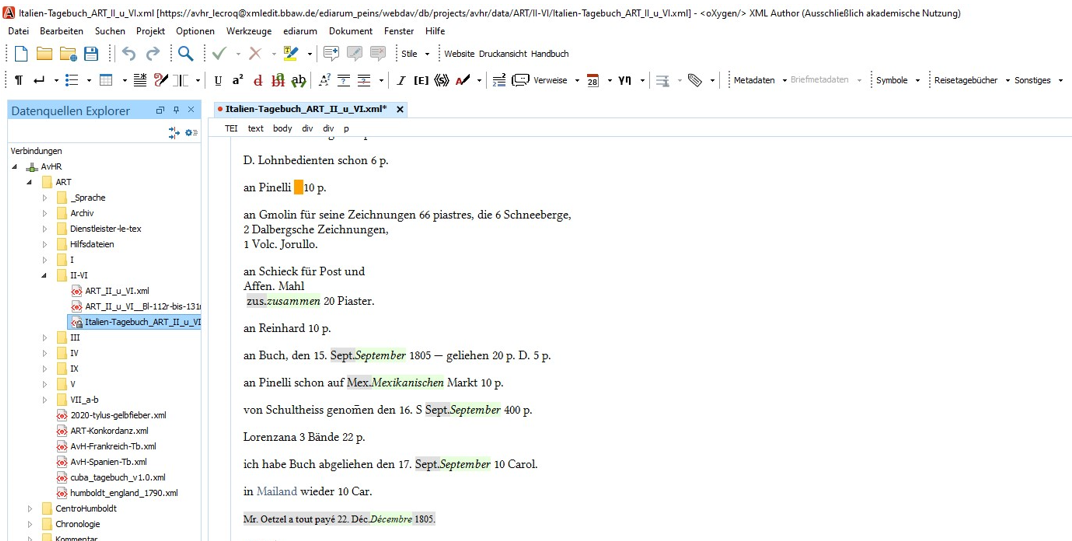
\includegraphics[scale=0.7]{img/ediarum_umgebung.png}
    \caption{Extrait du carnet de voyage d'Italie (1805) dans l'environnement ediarum.}
    \hfill
\end{figure}

Afin de s'adapter aux équipes d'éditions numériques de la \gls{bbaw}, \gls{telota} a développé un ensemble d'extensions pour ce logiciel, il s'agit d'ediarum. Cette extension vise à fournir un environnement optimisé pour travailler avec des transcriptions et leur balisage. Il permet à l'utilisateur de travailler avec des données \gls{xml} spécifiquement \gls{tei} en utilisant une interface utilisateur graphique qui propose un affichage \gls{wysiwyg}. Ces éditeurs ou traitements de texte \gls{wysiwyg} offrent une interface utilisateur qui permet de composer visuellement le résultat voulu. Ce sont des interfaces plus intuitives et par conséquent plus accessibles puisque l'utilisateur peut directement voir à l'écran ce à quoi ressemblera le résultat final. Grâce à cet environnement logiciel l'encodage devient plus simple et permet aux personnes des équipes d'éditions numériques n'étant pas ou peu familières avec le code brut \gls{xml} de pouvoir malgré tout travailler sur l'encodage des textes. 

\begin{wrapfigure}{r}{0.3\textwidth}
\centering
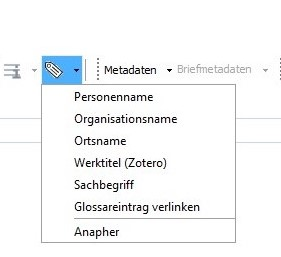
\includegraphics[width=0.3\textwidth]{img/ediarum_register.jpg}
\caption{Les différents index directement accessibles dans ediarum }
\vspace{-10pt}
\end{wrapfigure}

Les diverses fonctionnalités apparaissent sur une barre graphique semblable à celle que les utilisateurs ont l'habitude d'utiliser sur d'autres logiciels. Il est ainsi possible d'encoder de manière intuitive les annotations, notes, ajouts, rayures, abréviations et autres spécificités du document de manière simple. Une icône apporte un accès aux index de lieux, de personnes et des oeuvres mentionnés permettant de rajouter les balises adaptées ainsi que les identifiants correspondants. L'interface graphique ediarum offre la possbilité d'ajouter des balises et des métadonnées sans avoir à modifier manuellement les fichiers \gls{xml}. 

Bien que certaines parties des modules ne sont actuellement disponibles qu'en langue allemande et que la documentation doit être améliorée, ediarum offre déjà aux chercheurs un moyen flexible et ouvert d'éditer leurs données \gls{tei}. Il s'agit également d'une ressource sur laquelle d'autres développeurs peuvent s'appuyer puisqu'ediarum est accessible en open source. En effet, après avoir été utilisé au sein des projets internes de la \gls{bbaw} pendant plusieurs années\footnote{\cite{noauthor_ediarum_nodate-1}}, les modules ont été successivement mis à disposition du public sur un \href{https://github.com/ediarum}{dépôt GitHub} qui comprend toutes les informations nécessaires concernant ediarum. Les modules d'ediarum peuvent ainsi être utilisés comme point de départ ou bien comme boîte à outils pour d'autres développeurs qui souhaiteraient créer des cadres personnalisés et spécifiques à des projets d'édition numérique. C'est au sein de cet environnement logiciel que les carnets de voyage d'Alexander von Humboldt ont été encodés par l'équipe de \textit{Alexander von Humboldt auf Reisen - Wissenschaft aus der Bewegung.}

\subsection{L'encodage général}
La version adaptée d'oxYgen XML Author acompagnée d'ediarum est utilisé afin de saisir et d'éditer les données. Les données sont stockées dans la base de données \gls{xml} gratuite \href{http://www.exist-db.org/exist/apps/homepage/index.html}{eXistdb}. Avec le serveur web Jetty, il sert également de base à l'édition numérique qui a été réalisée avec les langages XQuery, \gls{xsl}T et XPath. 

L'\textit{edition humboldt digital} suit un modèle d'édition numérique qui met en oeuvre une approche visuelle, textuelle et liée au contenu des sources manuscrites. Visuellement, les modifications textuelles apportées par l'auteur sont reproduites telles que le surlignage, les ratures, les annotations et corrections. 

\begin{wrapfigure}{l}{0.37\textwidth}
\centering
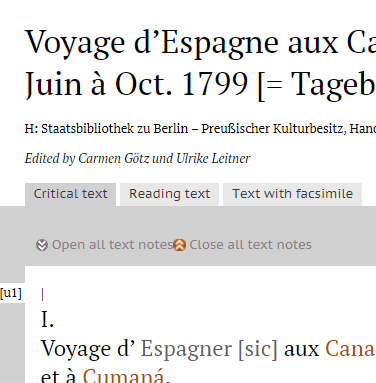
\includegraphics[width=0.37\textwidth]{img/edition_ongletslecture.png}
\caption{Les diverses approches textuelles accessibles sur le site de l'édition. }
\vspace{-10pt}
\end{wrapfigure}
Tous les textes édités sont également accompagnés de leur facsimilé numérisé dans la mesure du possible. L'état de conservation, de la numérisation et du cadre juridique sont des principaux freins à l'affichage d'un facsimilé des documents au sein de l'interface web. Le logiciel \href{https://robcast.github.io/digilib/}{digilib} développé au Max-Planck Institut pour l'histoire des sciences est utilisé pour afficher les facsimilés. L'approche textuelle, quant à elle, se compose en trois parties : un texte critique, un texte avec facsimilé qui contient tous les commentaires critiques des éditeurs et un texte de lecture qui vise à une présentation grand public et qui simplifie la typographie du document. L'approche liée au contenu se concentre sur la préparation d'un maximum d'informations contenues dans les textes sous forme de données structurées telles que les noms de personnes et de lieux, les titres d'oeuvre, les indications de mesures effectuées par Humboldt. Ces différentes approches textuelles des manuscrits sont directement accessibles sur le site de l'édition numérique avec un système d'onglet.

Des registres ont été également créés permettant d'indexer divers éléments au sein de l'édition : les personnes, les plantes et les lieux. La création de ces registres est concevable grâce notamment à un balisage constant de ces éléments par les éditeurs au sein de l'encodage ainsi qu'à l'utilisation d'identifiants pérennes vers des notices d'autorités. L'utilisation de ces identifiants dans l'encodage insère l'édition au coeur du web de données.

\section{Interopérabilité et web de données}
\label{sect:interEtLinkedData}
\subsection{Entre théorie...}
L'interopérabilité d'un document est un terme informatique désignant des documents capables de s'adapter et d'être utilisés facilement par d'autres systèmes. Synonyme de compatibilité, cette capacité permet notamment de faciliter la création d'un réseau et le transfert de données provenant de documents ou programmes différents.

L'interopérabilité de la \gls{tei} est en grande partie du au fait qu'il s'agisse d'un langage issu du \gls{xml}. Ce dernier est un métalangage et est spécialement conçu pour les données. Un des objectifs de la création de \gls{xml} était de favoriser les échanges et le partage des données entre machine et utilisateur. Ainsi, un fichier \gls{xml} est autodescriptif, extensible, interopérable et pérenne et est convertible en plusieurs autres formats grâce à des feuilles de style définies en \gls{xsl}. Il existe trois types d'interopérabilité : l'interopérabilité technique, l'interopérabilité sémantique et l'interopérabilité syntaxique. La première concerne la capacité des technologies à communiquer entre elles et à se comprendre et permet par exemple d'échanger des données  issues de normes bien définies ; tandis que la seconde assure le fait que la signification exacte des informations échangées soit compréhensible par n'importe quelle autre application. Pour assurer une interopérabilité sémantique, les deux côtés de l'échange doivent se référer à un modèle de référence d'informations communs. L'interopérabilité syntaxique concerne, quant à elle, la façon dont sont codées et formatées les données en définissant notamment la nature, le type et le format des informations échangées. 

Le \gls{xml} s'insère dans ce qu'on appelle le web sémantique puisqu'il offre la création de documents composés de données structurées. Le web sémantique permet aux machines de comprendre la sémantique c'est-à-dire la signification de l'information sur le web. Dans le web sémantique, les informations sont publiées accompagnées de métadonnées, fournissant ainsi un contexte dit sémantique. Le contenu de l'édition est alors enrichi avec des données interactives. Son sens est renforcé par des balises sémantiques et des liens directs vers des ressources externes ou vers les références citées. On parle alors du concept de \textit{semantic publishing} (éditorialisation sémantique), c'est-à-dire de l'enrichissement sémantique des publications et éditions scientifiques. 

Le web sémantique met en oeuvre le web de données, appelé \textit{linked data} en anglais, qui consiste à lier et structurer l'information pour accéder simplement à la connaissance qu'elle contient déjà. Tim Berners-Lee le définit : "Les données du \textit{linked data} peuvent être traitées directement ou indirectement par des machines pour aider les utilisateurs à créer de nouvelles connaissances"\footnote{\cite{berners-lee_semantic_2001}}. Ses objectifs sont multiples :
\begin{itemize}
    \item mettre à disposition des données en utilisant des techniques standardisées qui garantissent l'interopérabilité
     \item relier les données entre elles et les rendre interprétables par les machines
     \item permettre aux données d'être partagées et réutilisées
\end{itemize}

Le web de données permet de relier non pas les documents (pages HTML par exemple) mais les données entre-elles et de les rendre exploitables par des machines. Il s'appuie notamment sur des standards d'informations qui sont ceux du web sémantique. Par conséquent, le web de données vise à favoriser la publication de données structurées sur le web dans le but de constituer un réseau global facilitant la navigation des utilisateurs au sein d'un espace d'information. 
\begin{figure}[h]
    \centering
    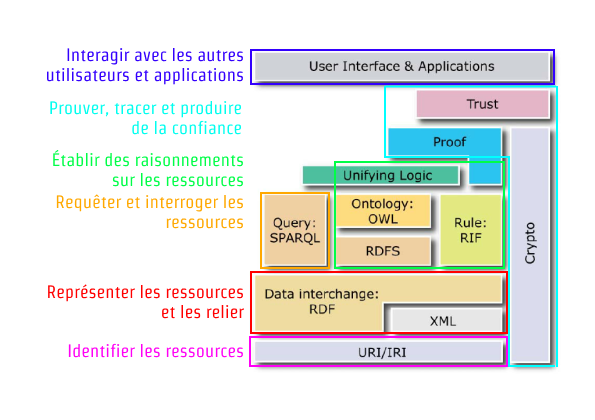
\includegraphics[scale=0.6]{img/semanticstack.png}
    \caption{L'architecture du Web sémantique ou \textit{semantic stack}. Source : \href{https://fr.wikipedia.org/wiki/Semantic_Web_Stack}{Wikipedia, Semantic Stack}}
    \label{fig:semanticStack}
    \hfill
\end{figure}

Il faut toutefois noter que le \gls{xml} ne constitue pas un modèle qui est entièrement adapté au contexte du web sémantique comme le souligne Grégory Fabre\footnote{Fabre Grégory, Marcotte Sophie, “L’organisation des métadonnées”, in : \cite[chapitre 5]{vitali-rosati_pratiques_2014}}. L'image ci-dessous permet de visualiser que le \gls{xml} doit impérativement être accompagné du \gls{rdf} afin d'offrir une mise en relation des sources. Ce dernier est un modèle de graphe qui décrit les ressources utilisées ainsi que les métadonnées. Toutefois, l'utilisation du \gls{xml} est une des portes d'entrée possible pour une édition historique de faire partie du web sémantique et donc du web de données. 

\subsection{...et pratique}
\label{subsec:miseEnPratique}
Une fois les concepts définis, il est intéressant de voir comme cela s'applique au sein d'une édition numérique scientifique. En tant que scientifique et botaniste, la diversité des plantes et des spécimens biologiques fait partie intégrante des notes écrites par Alexander von Humboldt dans ses carnets de voyage. En ce qui les concernent, aucune entrée distincte n'est enregistrée au sein d'un index stocké dans la base ediarum.BASE comme c'est le cas pour les personnes, lieux et institutions. Les noms scientifiques des plantes sont normalisés dans l'édition numérique. Pour chaque plante balisée dans l'encodage, elle est automatiquement ajoutée à la liste des références la concernant et est également automatiquement liée à diverses bases de données taxonomiques externes en utilisant divers services web et \gls{api}. Le service web \href{https://resolver.globalnames.org/}{\textit{Global Name Resolver}} permet de relier de manière automatique un nom scientifique à ces bases externes. Parmi ces dernières peuvent être mentionnées le \textit{\href{https://www.catalogueoflife.org/}{catalogue of life}}, la \textit{\href{https://www.biodiversitylibrary.org/}{biodiversity heritage library}} ainsi que le \textit{\href{https://www.ipni.org/}{international plant names index}}. L'index des plantes proposés sur le site de l'édition numérique est donc créée de manière entièrement dynamique.

Pour ce qui est des personnes, lieux et institutions, les registres proposés sur le site de \textit{edition humboldt digital} se forment d'une manière différente et s'alignent sur des référentiels externes. Au sein de l'encodage, une personne est balisée dans un \texttt{<persName>} dans laquelle l'attribut \texttt{@key} stocke l'identifiant interne de l'édition commençant forcément par un \texttt{H}, comme par exemple: \texttt{<persName key="H0012737">James Arnold</persName>}. Cet identifiant se réfère directement à une entrée au sein de l'index de personne. Les index des personnes, des lieux et des institutions sont traités et stockés en \gls{xml}-\gls{tei} dans l'environnement ediarum.BASE. Chaque entrée possède un identifiant unique et permanent. Elle est également pourvu d'un ou plusieurs identifiants provenant de divers services externes afin de permettre une interopérabilité de l'édition. Une courte description concernant l'objet ou la personne encodée est rédigée et accompagne les données de base.

Prenons donc plus précisément l'exemple d'une entrée au sein de l'index des personnes. Chaque nouvelle entrée dans l'index est encodée dans une balise \texttt{<person>}. Un identifiant est automatiquement généré dans l'attribut \texttt{@xml-id} et qui sera par la suite normalisé. S'il s'agit d'un personnage fictif ou mythologique, alors l'attribut \texttt{@role} est ajouté et accepte les valeurs \texttt{"fictional"} et \texttt{"mythological"}. Le nom et le prénom de la personne sont enregistrés dans la balise \texttt{<persName type="reg">}, la valeur de \texttt{@type} signifiant \textit{regular}. Les variantes ou les noms alternatifs sont chacun stockés dans une balise \texttt{<persName>} distincte où les attributs \texttt{@type="alt"} pour alternatif et \texttt{@subtype} sont acceptés. Les dates de naissance et décès sont indiquées dans les balises adaptées à savoir \texttt{<birth>} et \texttt{<death>}. Une note, plus ou moins longue en fonction des besoins d'explications de l'édition, peut également accompagner cette entrée. Ainsi, des informations détaillées concernant leur vie et activité professionnelle y sont mentionnées. L'édition utilise des référentiels de données normés divers. Une personne est liée à son identifiant \gls{gnd} ou en anglais \textit{integrated authority file} du site de la \textit{Deutsche Nationalbibliothek} ou bien à un identifiant \gls{viaf} quand cette personne ne possède pas d'identifiant \gls{gnd}. L'identifiant \gls{gnd} est pour l'Allemagne ce que l'identifiant de la \gls{bnf} est pour la France. Particulièrement employés par les bibliothèques, les identifiants \gls{gnd} sont de plus en plus utilisés par les centres d'archives, les musées et autres institutions culturelles et scientifiques. Son emploi permet de relier les données de diverses origines entre elles. Elles forment un réseau de données interopérables par les machines.
Une entrée complète liée à un identifiant \gls{gnd}  au sein du registre des personne se présente comme suit : 

\newpage
\begin{minted}[fontsize=\footnotesize]{XML}
<person xml:id="H0004159" role="mythological">
    <idno type="uri">http://d-nb.info/gnd/118557513</idno>
    <persName type="reg">
        <name>Jesus Christus</name>
    </persName>
    <persName type="alt">
        <name>Jesus von Nazareth</name>
    </persName>
    <note>Religionsstifter, Sohn Gottes (Gottvaters), sein Wirken wird im Neuen
        Testament der Bibel geschildert</note>
</person>
\end{minted}

L'identifiant \gls{gnd} est balisé au sein \texttt{<idno>} et est stocké sous forme d'\gls{uri}. Encoder un lieu au sein de l'édition fonctionne sur le même principe que l'encodage d'une personne : avec un registre, un identifiant interne et une ressource externe liée au sein d'une balise \texttt{<idno>} stockée également sous forme d'\gls{uri}. Le référentiel auquel les lieux de l'édition s'alignent est GeoName qui proposent des identifiants pérennes.

Au sein du web sémantique, l'\gls{uri} se situe à la base de son architecture\footnote{Voir \autoref{fig:semanticStack}.} car tous les hyperliens du Web sont exprimés sous cette forme.
Quatre piliers du web de données définis par Tim Berners-Lee sont fondés sur les bonnes pratiques de l'utilisation de ces \gls{uri}\footnote{Voir l'article \href{https://fr.wikipedia.org/wiki/Web_des_données}{Wikipédia sur le Web de données}.} :
\begin{itemize}
    \item utiliser des adresses \gls{uri} uniques pour identifier les choses
    \item utiliser des adresses \gls{uri} \gls{http}
    \item fournir à travers l'adresse \gls{uri} des renseignements exploitables, lisibles par les humains et machines en s'appuyant sur des formats ouverts
    \item mailler l'adresse \gls{uri} initiale en lui associant des adresses \gls{uri} externes et ce, pour améliorer la navigation de l'utilisateur sur le web
\end{itemize}
Ainsi, l'\gls{uri} identifie une ressource physique ou abstraite dont la syntaxe respecte une norme d'Internet et doit pouvoir l'identifier de manière permanente. Il faut différencier \gls{url} et l'\gls{uri}. En effet, l'\gls{url} identifie ce qui existe sur le web et permet d'identifier une ressource web comme une page. Une \gls{uri} est, quant à elle, attribuée à toute ressource et permet de l'insérer dans le web de données. Pour résumer, l'\gls{uri} est l'identifiant unique qui faire référence à une ressource tandis que l'\gls{url} est le chemin d'accès pour obtenir une représentation de cette ressource. En effet, dans le \textit{linked data}, l'\gls{uri} doit être interrogeable via le protocole \gls{http}. Par conséquent, l'\gls{uri} doit pouvoir s'exprimer par une \gls{url}. 

Il faut toutefois préciser que l'ajout de références par l'hyperlien doit être faite de manière judicieuse comme le mentionne Romain Wenz\footnote{\cite{wenz_hypertextualisation_2012}}. Si les références sont évidentes alors elles sont sans intérêt. Elles deviennent inutiles si elles sont trop complexes ou nombreuses. La référence d'une ressource doit impliquer une forme d'éclaircissement. Elle doit être explicative mais doit également pouvoir aller au-delà de la simple citation de sources. Les références doivent offrir de nouvelles possibilités de découverte sous une forme d'association d'idées.
Le réseau formé par cet ensemble de liens ne relève pas du hasard. En effet, les liens correspondent à chaque fois à des citations volontaires de la part des éditeurs de l'édition numérique. Ils sont également explicites et significatifs puisqu'ils ont pour but d'apporter plus de sens à l'utilisateur. 

L'alignement des données à un référentiel externe est possible grâce à l'utilisation d'identifiants de notice d'autorité au sein de l'édition, comme l'identifiant \gls{gnd} ou \gls{viaf} ou encore de service web tierces comme \textit{Global Name Resolver}. Ces identifiants permettent de proposer des données interopérables et de s'insérer au sein du web de données. Cette démarche d'alignement à des référentiels vise à favoriser la recherche d'information, le partage et la citation. Les liens qui sont crées entre les différents référentiels permettent d'exposer des données plus riches, plus fiables, pérennes et interopérables. Les référentiels mentionnées dans ce chapitre sont loin d'être les seules ressources externes utilisées au sein de l'\textit{edition humboldt digital}(ehd). Cette dernière s'insère dans un véritable réseau en utilisant un grand nombre de services web, de données et référentiels externes divers.


\chapter{Les données externes et leur accessibilité}
\section{L'utilisation au sein de l'\textit{edition humboldt digital} de données et services web tierces }
\chaptermark{L'utilisation de données et services tierces}
\subsection{Définitions}
Sont qualifiées de données externes toutes les données qui ne sont pas générées par l'organisation et qui sont accessibles via des sources extérieures à l'organisation-même. Les données peuvent être achetées, échangées ou mises à disposition de tous gratuitement. Ces dernières sont considérées comme ouvertes à tous dans le cadre des politiques d'\textit{open data}. 
\subsubsection{L'importance de l'\textit{open data}}
L'\textit{open data} est l'ouverture des données, c'est-à-dire la mise à disposition gratuite dans des formats techniques réutilisables. Les données sont diffusées de manière structurée. La loi Valter précise également que les données doivent être diffusées publiquement en ligne dans un standard ouvert qui est aisément réutilisable. Les données, quant à elles, doivent être complètes et de qualité c'est-à-dire qu'elles doivent être brutes et accompagnées de leurs métadonnées\footnote{\cite{castets-renard_open_2016}}. 
Le concept de l'\textit{open data} comprend deux notions complémentaires\footnote{\cite{wenz_lopen_2016}} :
\begin{itemize}
    \item le droit de réutiliser les données en question (ouverture juridique garantie par une licence ouverte)
    \item la possibilité technique qui rend possible les échanges avec d'autres projets ou communautés conduisant ces entités à vérifier la qualité de leur production de données et par conséquent à améliorer son propre processus grâce à l'\textit{open data}
\end{itemize}
Les licences ouvertes et gratuites qui garantissent l'ouverture juridique des données sont diverses. Elles sont en mesure de répondre aux besoins d'une ouverture des données dans le domaine des humanités numérique et dans le cadre de l'\textit{open data}. Les plus courantes sont la Creative Commons 4.0 et l'\gls{odbl} de l'Open Knowledge Foundation. La première est centrée sur le droit d'auteur tandis que la seconde peut être appliquées aux bases de données.

Il faut cependant dissocier le \textit{linked data} c'est-à-dire le web de données et l'\textit{open data}, les données ouvertes. Ces deux concepts sont néanmoins particulièrement liés puisque les institutions qui publient des informations en ligne le font pour permettre leur diffusion large. Si elles le font sans apporter des liens vers les informations d'origine alors elles deviennent invisibles pour le public. De même, si elles le font sans ouvrir les données en question, elles créent une insécurité juridique pour les utilisateurs et seront soit contournées soit considérées comme inutiles\footnote{\cite{wenz_lopen_2016}}.
La mise à disposition des données d'une institution par l'intermédiaire d'\gls{api} permet de créer des applications ou des fonctionnalités que le site d'origine n'aurait pas nécessairement implémentées. Il faut néanmoins noter un risque : des applications peuvent être dépendantes de données externes et de service web dont on ne peut garantir la pérennité et parfois leur bon fonctionnement.

\subsubsection{L'interface de programmation applicative ou API}
La mise à disposition des données favorise la création d'\gls{api}. Dans le web de données, une \gls{api} permet à un système source d'exposer ses données à des fins d'exploitation par d'autres systèmes. Il s'agit d'un ensemble normalisé de classes, de méthodes, de fonctions et de constantes qui sert de façade par laquelle un logiciel offre des services à d'autres logiciels. 
Dans ce domaine, les bibliothèque se sont longtemps contentées de mettre en place un serveur \gls{sru} pour rendre interrogeables leurs données bibliographiques\footnote{\cite{tomic_usage_2014}}. Elles sont bien souvent accompagnées d'une description qui spécifie comment les clients peuvent se servir des fonctionnalités du serveur\footnote{La description de l'\href{https://api.bnf.fr/fr/api-sru-catalogue-general}{API SRU du catalogue de Bibliothèque nationale de France} est un bel exemple, étant particulièrement détaillée et fournie. Son interface permet de guider au mieux l'utilisateur non confirmé dans le domaine des API. }. Afin d'utiliser les \gls{api} et d'avoir accès aux données de l'institution source, il faut souvent déclarer son projet de développement auprès de la plateforme dans le but d'obtenir une clé d'authentification appelée \textit{consumer key}. Cette déclaration est de nature contractuelle et engage le client à suivre les conditions générales de la politique de développement\footnote{\cite{francony_leditorialisation_2018}}. 

\subsection{Les services web et données externes : l'édition numérique au sein d'un large réseau}
Au sein de l'\gls{ehd} de nombreuses \gls{api} sont utilisées, insérant l'édition numérique dans un véritable réseau de services web et d'utilisation de données tierces. Une infographie a été réalisée par le projet \textit{Alexander von Humboldt auf der Reisen} afin de faire voir ce réseau et rend compte des services exploités\footnote{N'hésitez pas à vous référer à l'annexe en question, \autoref{fig:donneesReseau}.}. En plus d'exposer les diverses ressources externes employées au sein de l'édition numérique, plusieurs captures d'écran de l'interface seront introduites dans cette description afin de présenter leur affichage dans l'interface web et la manière dont l'utilisateur peut y accéder.

\begin{wrapfigure}{r}{0.7\textwidth}
\centering
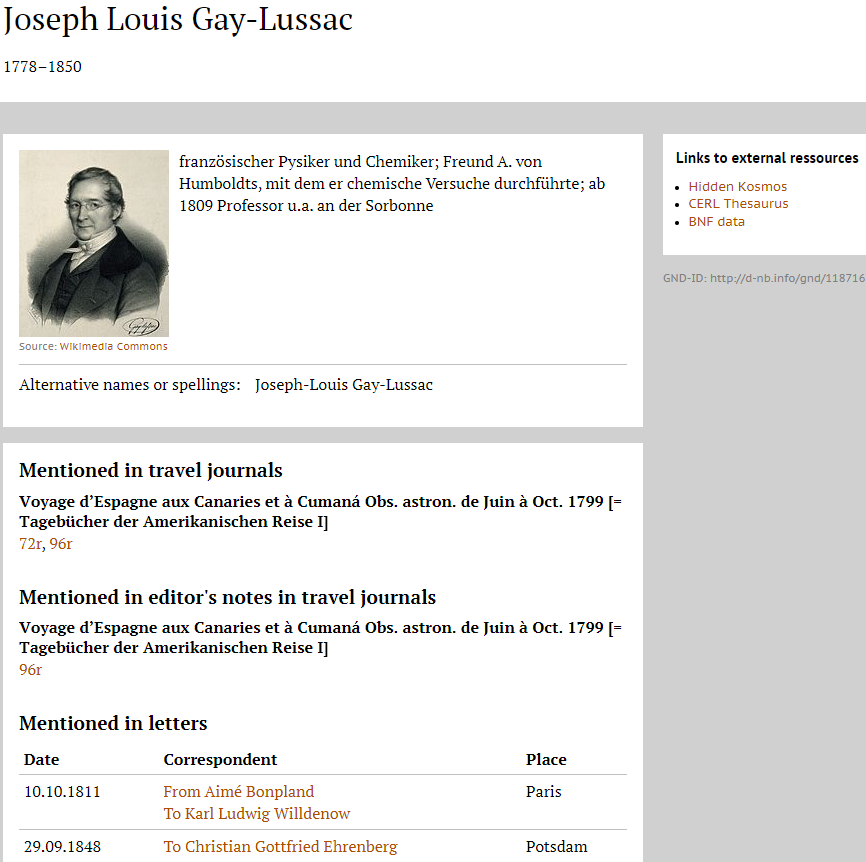
\includegraphics[width=0.7\textwidth]{img/portrait_gaylussac.png}
\caption{Gay-Lussac dans le registre des personnes. Capture d'écran de l'interface de l'édition numérique.}
\end{wrapfigure}

Dans les parties précédentes ont été évoqués les identifiants externes utilisés au sein de l'édition permettant de lier les données de l'édition avec des données externes et ainsi de faire partie du web de données. L'identifiant \gls{gnd} permet de faire référence à des personnes physiques. Ce même identifiant est utilisé afin d'importer les portraits de personnes issues de Wikimedia Commons. Ces portraits sont directement visibles pour l'utilisateur dans l'interface web. Toutes les informations relatives à la personne sélectionnée et tous les liens externes qui s'y réfèrent sont accessibles sur l'interface de l'édition numérique. La création de cette page résulte de la combinaison d'informations issues de sources diverses : le portrait provenant de Wikimedia Commons, la présentation de la personne tirée du registre de l'édition, les liens situés à droite vers des ressources externes. Tous ces liens apportent davantage d'informations sur le personnage présenté. En dessous de la présentation de la personne sont listées ses mentions au sein de l'édition. Dans ce cas précis, il s'agit des mentions de Gay-Lussac au sein des carnets de voyage écrits par la main de Humboldt, ainsi que ses mentions dans les commentaires des éditeurs. Cette liste est donc générée grâce au fait que le nom de cette personne a été systématiquement balisé par les éditeurs\footnote{Voir la \autoref{subsec:miseEnPratique}} dans l'encodage. 

\begin{wrapfigure}{l}{0.7\textwidth}
\centering
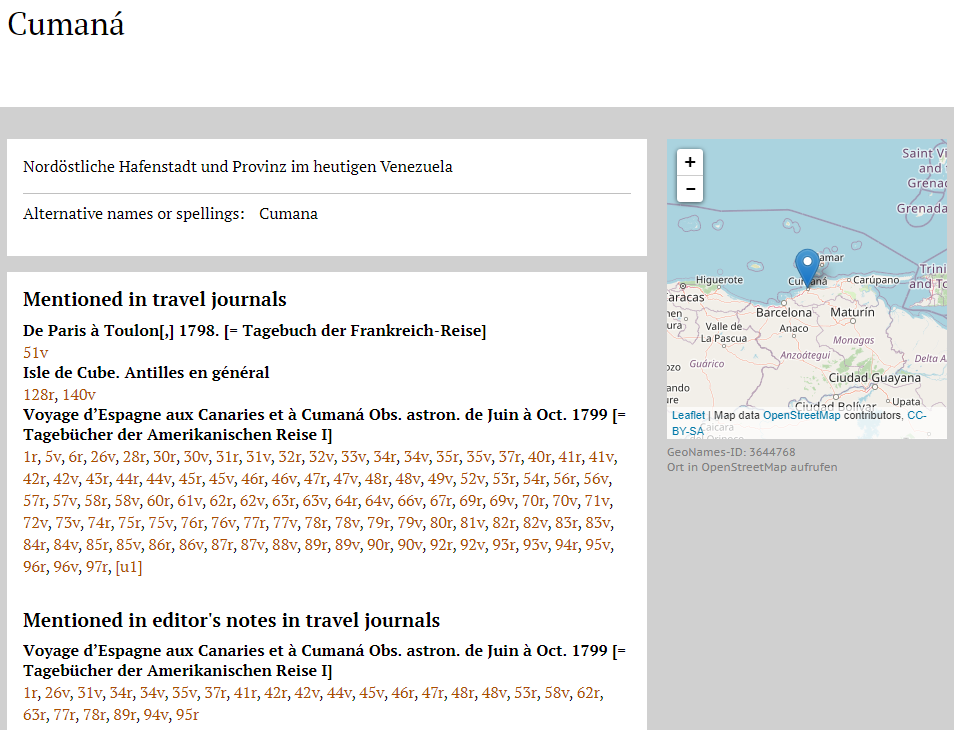
\includegraphics[width=0.7\textwidth]{img/index_cumana.png}
\caption{La ville de Cumana dans l'index des lieux de l'édition numérique}
\end{wrapfigure}
Par ailleurs, deux applications sont nécessaires afin de pouvoir présenter sur une carte un lieu sélectionné dans l'interface web. L'emploi de l'identifiant GeoName dans l'encodage permet également de récupérer ses geopoints qui sont ses points de géolocalisation. En plus d'une note présentant la lieu, le pays dans lequel il se situe et ses noms alternatifs, le lieu sélectionné dans l'index des lieux est présenté aux lecteurs de l'édition numérique sur une carte qui provient de l'application \href{https://www.openstreetmap.org/}{Open Street Map}. Tout comme pour les personnes, la présentation du lieu et ses noms alternatifs proviennent directement du document \gls{xml}-\gls{tei} encodé par l'équipe du projet \textit{Alexander von Humbold auf der Reisen}. Les mentions de ce lieu au sein des divers carnets de voyages et des notes des éditeurs sont listées sous sa présentation générale.

En plus de ces données externes, l'emploi de services web et de standards permet à l'édition numérique de s'insérer dans des réseaux spécifiques. Grâce à l'utilisation du standard \gls{dtabf}\footnote{Voir la \autoref{sub: tei_dtabf}}, l'édition s'insère dans le corpus des institutions qui ont recourt également ce format. Les lettres éditées au sein de l'\textit{edition humboldt} sont encodées dans le \gls{cmif} qui est issu du \gls{xml}-\gls{tei}. Ce format est notamment employé dans le projet correspSearch\footnote{Le projet correspSearch et le \gls{cmif} font l'objet d'un chapitre complet, voir le \autoref{chap:cSBesoins}} initié par la \gls{bbaw}. La plateforme correspSearch met à disposition la correspondance des personnes de diverses époques qui ont été éditées en version imprimée ou numérique. Il est ainsi possible de retrouver les lettres de l'\gls{ehd} sur le site de correspSearch comme toutes les correspondances éditées au sein des éditions numériques de \gls{bbaw}. Par ailleurs, la ressource archivistique est indiquée dans l'\textit{edition humboldt digital}. Le lien vers le Kalliope-Verbundkatalog est indiqué au sein de l'encodage dans la balise \texttt{<sourceDesc>}. Le lien vers le catalogue en ligne est directement cliquable au sein de l'interface web. En cliquant sur ce lien, l'utilisateur accède a davantage d'informations concernant le document physique et peut également avoir accès à la numérisation de ce document quand celle-ci existe. 
\begin{figure}[h!]
    \centering
    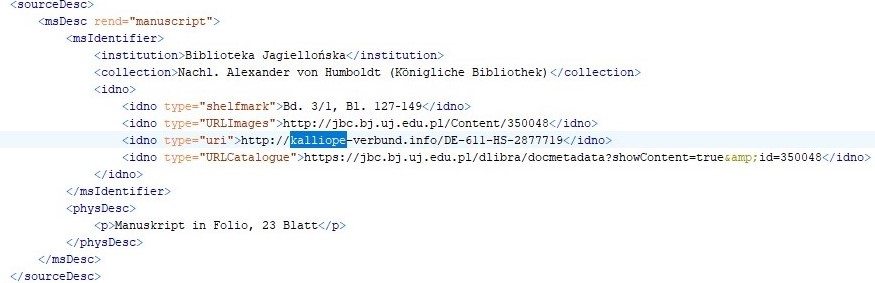
\includegraphics[width=15cm]{img/edh_kalliope_xml.jpg}
    \caption{Le lien vers le Kalliope-Verbundkatalog dans le \texttt{<sourceDesc>}}
    \label{fig:kalliopeLinkXML}
    \hfill
\end{figure}
\begin{figure}[h!]
    \centering
    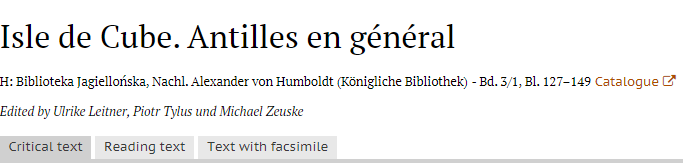
\includegraphics[width=13cm]{img/edh_kalliopelink.png}
    \caption{Le lien vers le Kalliope-Verbundkatalog cliquable dans la version numérique de l'édition}
    \label{fig:kalliopeLinInterface}
    \hfill
\end{figure}

Les données de la correspondance accessibles sur ce catalogue archivistique en ligne font par ailleurs partie des données qui ont été exploitées au cours du stage pour les projets menés. Ensemble, étudions maintenant ces données.

\section{Les données manipulées au cours du stage}
\label{sect:donnéesStage}
\subsection{Kalliope-Verbundkatalog}
\label{sub:kalliope}
\subsubsection{Présentation du Kalliope-Verbundkatalog}
Le Kalliope-Verbundkatalog est un catalogue numérique collectif et se situe dans la continuité  du  \gls{zka}, fondé en 1966 à Berlin Ouest. Les données à l'origine Kalliope étaient les 1,2 millions de fiches du \gls{zka} ainsi que les références de près de 450 institutions allemandes\footnote{\cite{noauthor_kalliope_nodate}}. La base de données \textit{ZKA online} a été développée de 2001 à 2003\footnote{\cite{noauthor_kalliope_nodate}}. Depuis octobre 2004, les fonds de base du catalogue concernant les fiches du \gls{zka} sont consultables en ligne. Le portail a été renommé par la suite Kalliope. Ce dernier est un outil de référence nationale Outre-Rhin pour les références archivistiques manuscrites.
Aujourd'hui ce sont environ 500 institutions comprenant des bibliothèques, des centres d'archives et des musées d'Allemagne mais aussi d'autres pays qui sont répertoriés comme institutions propriétaires et partenaires. La plupart des données hors Allemagne proviennent d'Autriche, Suisse et de personnes d'origine allemande ou germanophones situées dans d'autres pays tels que les États-Unis\footnote{\cite{noauthor_kalliope_nodate}}.

\begin{table}[h!]
    \centering
    \renewcommand*{\footnoterule}{}
    \begin{tabular}{|c|c|c|}
    \hline
         Année & Documents & Institutions \\
         & & partenaires\footnotemark \\ \hline
         2010 & 1 530 600 & 54\\
         2012 & 1 610 156 & \\
         2014 & 2 200 443 & \\
         2015 & 2 350 000  & 102 \\
         2021 & plus de 3 millions & 950 \\\hline
    \end{tabular}
    \caption{Qunatité des documents et des institutions partenaires du Kalliope-Verbundkatalog}
    \label{tab:docsKalliope}
\end{table}
\footnotetext{Ce tableau a été réalisé à partir des chiffres présentés sur : \cite{noauthor_kalliope_nodate} ; \cite{noauthor_kalliope_opac_2014}}

L'ensemble de la base de données a augmenté d'environ 20\% par an ces quatre dernières années\footnote{\cite{noauthor_kalliope_nodate}}. Les données sont mises à disposition en format \gls{xml}-\gls{ead} grâce à une \gls{api} et plus particulièrement un serveur \gls{sru}.

\subsubsection{Des requêtes aux données}
Sur le serveur \gls{sru} du Kalliope-Verbundkatalog, l'utilisateur peut récupérer les données qui l'intéresse sous format \gls{dc} ou \gls{mods}.
Le \gls{dc} sert à décrire des documents de manière standardisée permettant une interopérabilité minimale. Le \gls{mods}, quant à lui, est issu du métalangage \gls{xml}. Il a été conçu à la croisée du format MARC21, considéré comme complexe, et le \gls{dc} qui propose une simplicité de jeu de métadonnées\footnote{\cite{noauthor_metadata_2020}}. \gls{mods} structure des données bibliographiques en \gls{xml} notamment dans le cadre de projet de catalogues bibliographiques ou de portails documentaires. Il contient en effet de nombreux éléments qui permettent d'indiquer les données au sujet de la description de la version numérique d'un document. 

Les deux types de format ont été récupérés et utilisés au sein des projets menés au cours de mon stage. Dans un premier temps, le \gls{dc} proposait suffisamment d'informations afin de mettre en place des fonctions de recherche et des visualisations. Néanmoins, ce format n'apportait pas assez de métadonnées pour le second projet, à savoir le développement d'un outil de corrélation entre deux sets de données. En effet, dans le format \gls{mods}, il est possible de récupérer les identifiants \gls{gnd} des correspondants épistolaires\footnote{Voir l'annexe \ref{annexe:MODSetDC}.} ce que ne propose pas le \gls{dc}. Ainsi, le choix du format implique de savoir ce que l'on souhaite faire de ces données. Il est superflu de récupérer le maximum d'informations quand le projet ne nécessite pas toutes ces données. Dans la pratique et plus particulièrement dans la requête, le choix du format doit y être mentionné afin de récupérer les données dans le format souhaité.

Décortiquons une requête sur le serveur \gls{sru} du Kalliope-Verbundkatalog afin de comprendre son fonctionnement. Prenons cet exemple : \\
\texttt{https://kalliope-verbund.info/sru?\textcolor{violet}{version=1.2}\&\textcolor{Lavender}{operation=searchRetrieve}\&\newline \textcolor{Peach}{query=}\textcolor{Emerald}{ead.addressee.gnd\%3D\%3D\%22118554700}\%22+AND+\textcolor{YellowGreen}{ead.genre\%3D\%3D\%22Brief}\newline\%22\&\textcolor{purple}{maximumRecords=4000}\&\textcolor{Salmon}{recordSchema=mods}}
\begin{itemize}
    \item \texttt{\textcolor{violet}{version=1.2}} indique la version de la demande du client et constitue une déclaration de ce dernier selon laquelle il souhaite que la réponse reçue soit égale ou inférieure à cette version. Ce paramètre \texttt{version} est obligatoire.  
    \item \texttt{\textcolor{Lavender}{operation=searchRetrieve}} est le type d'opération effectuée sur le serveur. L'opération \texttt{searchRetrieve} est la principale opération du \gls{sru}. Elle permet au client de soumettre une demande de recherche et d'extraction de données correspondantes auprès du serveur. Cet élément est obligatoire dans une requête.
    \item \texttt{\textcolor{Peach}{query=}} indique le début de la requête. 
    \item \texttt{\textcolor{purple}{maximumRecords=5000}} permet de préciser le nombre d'enregistrements à renvoyer. La valeur doit être égale ou supérieure à 0. En outre, si le nombre contenu dans la base est inférieur au nombre indiqué, le serveur renvoie un nombre d'enregistrements inférieur à celui demandé mais il ne doit pas en renvoyer plus. Ce paramètre est optionnel. Quand il n'est pas indiqué alors le serveur envoie le nombre d'enregistrements définit par défaut. Cette valeur varie en fonction du paramétrage du serveur par l'institution. Dans cette requête exemple, il est indiqué 4000 enregistrements maximum afin de récupérer en une seule requête les enregistrements de toutes lettres correspondantes. Or, le serveur renvoie 3236 entrées.
    \item \texttt{\textcolor{Salmon}{recordSchema=mods}} indique le schéma dans lequel les enregistrements doivent être renvoyés. Ici, nous désirons un format MODS. Si le format \gls{dc} est souhaite alors \texttt{dc} devra être indiqué à la place de \texttt{mods}. 
\end{itemize}
On requête sur deux éléments distincts : \texttt{\textcolor{Emerald}{ead.addressee.gnd\%3D\%3D\%22118554700\%22}} et \texttt{\textcolor{YellowGreen}{ead.genre\%3D\%3D\%22Brief}}. Ces deux éléments sont articulés par un opérateur logique \texttt{AND}. On recherche par conséquent tous les enregistrements qui sont du genre "lettre" (\textit{Brief}) et dont le destinataire (\textit{addressee}) a comme identifiant \gls{gnd} le nombre 118554700 qui est l'\href{http://d-nb.info/gnd/118554700}{identifiant \gls{gnd} d'Alexander von Humboldt}. Une seconde requête a ensuite été effectuée afin de récupérer toutes les lettres écrites par Alexander von Humboldt.

\subsection{Société Américaine de Philosophie (APS)}
\label{sub:APS}
Originellement, l'\gls{aps} était un cercle de discussions fondé au milieu du XVIII\textsuperscript{e} par Benjamin Franklin dans la ville de Philadelphie. Débats scientifiques, publications, création d'une bibliothèques, les activités y était diverses\footnote{\cite{noauthor_societe_2020}}. Alexander von Humboldt en était l'un des membres en ayant été élu à la fin de son expédition américaine\footnote{\cite{noauthor_alexander_2021}}. 

Aujourd'hui la bibliothèque de l'\gls{aps} abrite plus de treize millions de manuscrits, 350 000 volumes et périodiques, 250 000 images et des milliers d'heures de bandes audio\footnote{\cite{noauthor_aps_library}}. Grâce à ces fonds, l'\gls{aps} est considérée comme l'une des premières institutions à documenter l'histoire naturelle aux XVIII\textsuperscript{e} et XIX\textsuperscript{e} siècles. Outre les collections de manuscrits remarquables telles que celle des documents de Benjamin Franklin, les journaux de Lewis et Clark ou la correspondance de Charles Darwin, l'\gls{aps} abrite notamment la plus grande collection de documents manuscrits et imprimés d'Alexander von Humboldt des États-Unis.  

L'\gls{aps} propose une bibliothèque en ligne qui permet aux utilisateurs de découvrir les collections numérisées. En son sein, seulement quelques dizaines de manuscrits d'Alexander von Humboldt sont disponibles car la plupart des documents du scientifiques conservés aux archives de l'\gls{aps} ne sont pas numérisés. Les données de ces numérisations sont téléchargeables dans un fichier \gls{csv}, accessible directement par un bouton sur l'interface de la bibliothèque numérique. Une \gls{api} est également proposée aux utilisateurs et les données sont récupérables en \gls{xml}-\gls{ead}. La collection d'Alexander von Humboldt contient environ 250 documents. Le détail de son contenu est visible sur le site \href{https://search.amphilsoc.org/collections/view?docId=ead/Mss.B.H88-ead.xml;query=Alexander\%20von\%20Humboldt}{search.amphilsoc.org}. Pour chaque document, diverses informations sont mentionnées : la personne qui est productrice de ce dernier, la date, la description physique, le lieu de conservation de l'original quand il s'agit d'une copie, le lieu de production ainsi que la typologie du document. Parfois quelques lignes résument le contenu du document concerné. En étudiant les documents de cette collection, on remarque que plusieurs dizaines de lettres y sont conservées. Celles-ci sont intéressantes pour le projet que nous devons mener. 


\subsection{Catalogue général de la Bibliothèque nationale de France}
\label{sub:BNF}
La France entre officiellement dans l'\textit{open data} en 2011 avec l'ouverture du site national \href{https://www.data.gouv.fr/fr/}{data.gouv.fr}. La \gls{bnf} y intègre toutes les données structurées dans les formats du web sémantique et les diffuse dans le projet \href{https://data.bnf.fr/}{data.bnf.fr}. Les objectifs de ce projet sont multiples\footnote{Voir le site de \href{https://data.bnf.fr/en/about}{Data BnF}.} :
\begin{itemize}
    \item accroître l'exposition des données de la \gls{bnf} sur le web
    \item fédérer les données de la \gls{bnf} au sein et au-delà des catalogues
    \item contribuer à l'échange de métadonnées par la création de liens entre les ressources structurées et de référence
    \item faciliter la réutilisation des métadonnées par des tiers avec la garantie que ces dernières se trouvent sous licence ouverte.
\end{itemize}

C'est à partir de 2014 que toutes les métadonnées issues des catalogues de la \gls{bnf} sont devenues librement réutilisables\footnote{\cite{wenz_lopen_2016}}. Cette ouverture se limite aux données descriptives c'est-à-dire aux métadonnées issues des catalogues et inventaires qui sont plus simples à extraire et diffuser. Il est devenu impératif d'exposer les données numériques dans des formats qui permettent aux utilisateurs de les réutiliser. Ce projet intègre des données produites en Intermarc pour les catalogues de livres, \gls{xml}-\gls{ead} pour les inventaires d'archives et\gls{dc} pour la bibliothèque numérique\footnote{\cite{databnf_semantic_nodate}}. Les données sont modélisées et regroupées par des traitements automatiques puis sont publiées dans les standards \gls{rdf}.

Le site data.bnf.fr met en avant des informations précises et structurées. Ces informations qui sont des ressources pertinentes sont regroupées autour de concepts comme celui d'auteurs, d'oeuvres ou de thèmes. Le navigateur évolue parmi les données provenant de sources diverses et accède au contenu des catalogues de manière immédiate. Cela est possible car la \gls{bnf} fournit des \gls{uri} pour les ressources grâce à des identifiants pérennes attribués selon le mécanisme \gls{ark} qui permet d'accéder à toutes les ressources que la bibliothèque propose.

La documentation accessible à l'utilisateur sur le site de data.bnf est riche que ce soit sur l'insertion du site au sein du web sémantique, sur les identifiants \gls{ark} ou encore sur la manière de se repérer dans le site. Tout est particulièrement bien documenté permettant aux utilisateurs de s'approprier de manière confortable les outils proposés par data.bnf. 

Le service \gls{sru} du Catalogue général de la \gls{bnf} permet d'interroger le catalogue général via des requêtes \gls{http}. L'ensemble des données sont récupérées dans différents formats bibliographiques encapsulés dans du \gls{xml}. Le service est libre d'accès et ne demande aucune authentification de la part des utilisateurs. Le \gls{sru} est interrogeable manuellement dans n'importe quel navigateur Internet et peut également être interrogé dans l'interface proposé sur le site de \href{https://api.bnf.fr/fr/api-sru-catalogue-general#/}{api.bnf.fr}. Les divers paramètres utilisables dans le \gls{sru} sont explicitement détaillés sur le site permettant à chacun d'interroger le serveur selon ses besoins. 

Ces données du Catalogue général sont différentes dans le format et leur niveau de détail de celles issues du Kalliope-Verbundkatalog et de l'\gls{aps}. Afin de pouvoir manipuler toutes ces données comme un ensemble unique, il faut les traiter dans le but de les exploiter. 

\chapter{Des données brutes aux données traitées}
\label{chap:brutesàtraitées}
La définition du traitement des données de Wikipédia permet de bien comprendre ce concept\footnote{\cite{wiki_traitement_2021}} :

\begin{changemargin}{1cm}{1cm}
\textit{
En informatique, le terme traitement de données renvoie à une série de processus qui permettent d'extraire de l'information ou de produire du savoir à partir de données brutes. [...]
Si la finalité n'est pas de présenter des résultats à un utilisateur humain, l'objectif du traitement de données est généralement d'offrir une information de plus haut niveau ou une information de meilleure qualité à un autre outil de traitement ou d'analyse. Ce traitement de l'information peut alors relever de la fusion de données, de l'extraction d'information ou de la transformation de la représentation. }
\end{changemargin}
Dans la phase de traitement, la donnée est nettoyée, compilée, croisée et analysée afin d'être enrichie.

\section{Nettoyer}
Interroger les \gls{api} permet de récupérer des données formatées et structurées mais qui sont considérées comme brutes car elles n'ont pas encore été traitées. Le nettoyage est une étape essentielle dans le processus du traitement des données. Il s'agit de nettoyer les doublons, les données obsolètes ou incomplètes, les erreurs. Chaque set de données récupéré doit ainsi être nettoyé dans le but poursuivre le processus du traitement des données et d'être exploitables dans les fonctions de recherche.

\begin{figure}[h!]
    \centering
    \caption{Entrée au sein du le fichier \gls{xml}-\gls{ead} des données de l'\gls{aps}}
    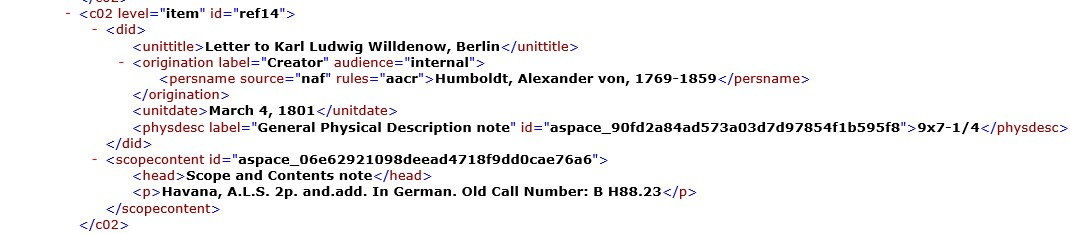
\includegraphics[scale=0.5]{img/APS-item.jpg}
    \hfill
\end{figure}

\begin{figure}[h!]
    \centering
    \caption{Entrée au sein du le fichier \gls{dc} issu du Kalliope-Verbundkatalog}
    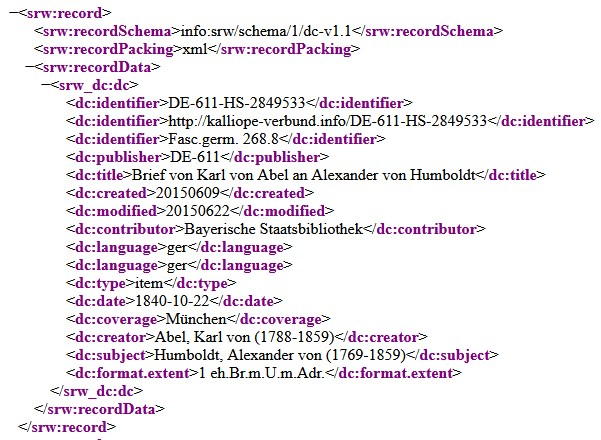
\includegraphics[scale=0.6]{img/kalliope-item.jpg}
    \hfill
\end{figure}

\begin{figure}[h!]
    \centering
    \caption{Entrées du CSV composé des données du Catalogue général de la \gls{bnf}}
    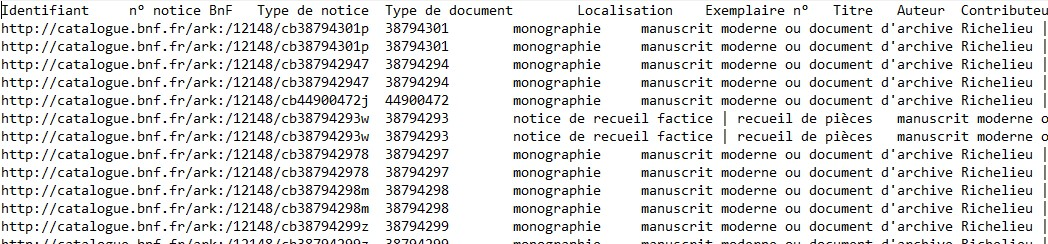
\includegraphics[scale=0.5]{img/bnfcsv.jpg}
    \hfill
\end{figure}


Par exemple, les données récupérées sur l'\gls{api} de l'\gls{aps} contiennent des documents de divers typologies : y sont présentes des lettres, des poèmes, une déclaration des bagages d'Alexander von Humboldt entrés sur le territoire des États-Unis... Dans le projet conçu, seules les lettres sont attendues. En outre, au sein de ce set de données, il faut extraite uniquement les données concernant les lettres, données qui seront ajoutées au set final c'est pourquoi 261 lettres ont été extraites du set de données source.

Par ailleurs, les données issues du Catalogue général de la \gls{bnf} contenaient vingt-quatre entrées différentes. L'étude de ces données met en évidence le fait que seuls douze identifiants \gls{ark} sont à définir et non vingt-quatre. Chaque ensemble de documents est conservé dans un carton qui a été également microfilmé. Ainsi, chaque document présente deux entrées dans les données issues de l'\gls{api} du Catalogue général : une entrée pour le document physique et une seconde pour son microfilmage. Un seul enregistrement est suffisant et est d'ailleurs intéressant pour notre projet. Par conséquent, les entrées représentant les documents microfilmés ont été retirés des données sources afin d'éviter les doublons dans le set de données traitées.

Les données issues du Kalliope-Verbundkatalog se distinguent, quant à elles, en deux sets : les lettres reçues par Alexander von Humboldt et celles envoyées par ce dernier. En tout, ce set contient exactement 4566 lettres : 3235 rédigées par Alexander von Humboldt et 1331 lettres reçues par ce dernier. Ces deux sets étaient particulièrement propres et seule une transformation du \gls{xml}-\gls{ead} vers \gls{json} a été nécessaire. Cette conversion de format s'insère dans la seconde étape du traitement de nos données: la fusion. 

\section{Fusionner}
Nous sommes à présent en possession de trois sets de données nettoyés : des données structurées dans un \gls{csv}, d'autres en \gls{xml}-\gls{ead} et les dernières en \gls{dc}. Chacune des structures est différente des autres. Or, les données doivent former un ensemble homogène et propre afin d'être exploitables au sein de notre projet. On parle alors de fusion de données. Cette dernière consiste à combiner plusieurs données issues de sources différentes, les compiler en un même set de données produisant une information plus sûre. 

Afin de fusionner les différents sets les uns avec les autres pour former un unique ensemble, ces sets de données doivent tous être dans un format identique. Ce format peut être utilisé uniquement pour l'étape de la fusion et ne plus être employé au sein du projet final. Choisir la manière dont les données seront stockées dans une application ou un projet informatique n'est pas une étape anodine et mérite réflexion. Conceptualiser et mettre en place une base de données très structurée comme une base de données relationnelle prend du temps. Toutefois utiliser une base de données relationnelle n'est pas toujours le plus adapté en fonction des besoins. Pour diverses raisons, l'équipe du projet a décidé de stocker toutes ces données dans un fichier commun \gls{json} qui présente plusieurs avantages :
\begin{itemize}
    \item Stocker en \gls{json} demande un faible besoin de place de stockage.
    \item \gls{json} est un format largement connu et les données y sont facilement manipulables.
    \item \gls{json} est un format également utilisé dans le projet développé en parallèle \textit{Humboldt Chronotopographie}\footnote{Voir la \autoref{sect:chronotopographie}}.
\end{itemize}

Le format \gls{json} est un format de données textuelles et qui structure des informations. Une des caractéristiques du document \gls{json} est qu'il comprend deux types d'éléments structurels : des ensembles de paires nommés clé/valeur et des listes ordonnées de valeur imbricables les unes dans les autres. Le document \gls{json} est plus facile à interpréter dans du code qu'un document \gls{xml}. Ce dernier impose le recours à des techniques souvent plus lourdes. En effet, pour interpréter un document \gls{xml} dans le langage Python il faut par exemple parcourir hiérarchiquement l'arbre \gls{dom}. 
Cet arbre \gls{dom} a d'ailleurs dû être parcouru afin de récupérer les données souhaitées dans le document \gls{xml}-\gls{ead} et \gls{dc} pour pouvoir les stocker dans le fichier \gls{json}. Des courts algorithmes rédigés en Python ont été programmés afin de convertir les divers formats en \gls{json}. Pour cela, la librairie \texttt{jxmlease} est particulièrement adaptée pour les conversions \gls{xml} vers \gls{json} ou vice versa. Une fonction de quelques lignes permet de convertir facilement les documents possédant une structure \gls{xml} vers \gls{json} :

\begin{figure}[h]
\begin{lstlisting}
def xml_to_json(file:str, data: list):
    """
    Convert a XML file to a JSON file 
    :param file: str
    :param data: list
    """
    with open(file, "w+") as f: 
        d = jxmlease.parse(data)
        json.dump(d, f)
        f.close()
\end{lstlisting}
\end{figure}


Pour le set de données en \gls{csv} de la \gls{bnf}, la fonction \texttt{DictReader} permet de le convertir en \gls{json} d'une manière tout aussi simple que ce que le permet la librairie \texttt{jxmlease} pour les fichiers \gls{xml} :

\begin{figure}[h]
\begin{lstlisting}
def csv_to_json(file: str, delimiter : str, outputfilename: str):
    """
    Convert a CSV file to a JSON file 
    :param file: str
    :param delimiter: str
    :param outputfilename: str
    """
    data = {}
    with open(file) as csv_file:
        reader = csv.DictReader(csv_file, delimiter)
        data = list(reader)
        writeJSON(outputfilename, data)
        csv_file.close()
\end{lstlisting}
\end{figure}

Une fois que les trois sets de données ont été nettoyés et convertis en \gls{json}, il est alors possible de les fusionner dans un fichier commun. Ce dernier, nommé \texttt{records.json} au sein de notre projet contient, après fusion, 4931 enregistrements de lettres provenant de trois sources différentes. 

 
\section{Enrichir}
Enrichir ses données est fortement lier à ce qu'on souhaite en faire. Parfois les enrichir est inutile mais bien souvent un enrichissement est nécessaire afin d'obtenir les résultats escomptés. Lors de cette étape, on peut créer des liens avec des ressources externes. On parle alors d'alignement avec des référentiels\footnote{\cite{fabry_publier_2017}}. Ce type de lien permet un rapprochement avec des entités similaires et augmente ainsi la visibilité du jeu de données au sein de web sémantique. 

Puisqu'un des objectifs du projet est de produire une visualisation cartographique, les geopoints des lieux des données doivent nécessairement venir compléter notre set. Afin que ce projet puisse s'insérer au sein d'\textit{Alexander von Humboldt auf Reisen}, l'identifiant interne de l'édition doit également être ajouté. L'\gls{api} \href{https://www.geonames.org/}{GeoName} permet de récupérer l'identifiant GeoName ainsi que les coordonnées géographiques d'un lieu. GeoName est une base de données géographiques mondiale. Elle contient plus de onze millions de noms de lieux. Afin de pouvoir utiliser son \gls{api}, l'utilisateur doit s'assurer d'être identifié. GeoName et son \gls{api} font déjà partie du réseau des services web utilisés au sein de l'édition numérique. J'ai ainsi pu profiter de l'identifiant de l'édition afin de récupérer les données dont j'avais besoin pour étoffer le set de lettres. 
Les données qui viennent enrichir notre set sont multiples. Pour chaque enregistrement au sein du set de données, doivent être rajoutés :
\begin{itemize}
    \item l'identifiant GeoName, l'identifiant interne de l'édition, la géolocalisation du lieu de convervation (clé \texttt{contributor} dans le fichier JSON)
    \item l'identifiant GeoName, l'identifiant interne de l'édition, la géolocalisation du lieu d'envoi ou de réception de la lettre (clé \texttt{coverage\_place})
\end{itemize}

Ainsi, algorithme a été rédigé afin de compléter les données concernant les lieux de conservation des lettres, puis un second second afin d'enrichir les données des lieux d'envoi de ces mêmes lettres. Afin de limiter le nombre de requêtes envoyé à l'\gls{api} GeoName, le programme recherche dans un premier temps si le lieu recherché n'est pas déjà enregistré dans l'index de lieu de l'édition. Un second index a été crée localement afin de pouvoir stocker les lieux qui ne sont pas dans l'index de lieu de l'édition et qui ont déjà été requêtés sur l'\gls{api} GeoName. Cela permet de ne pas effectuer deux requêtes différentes sur l'\gls{api} GeoName pour un même lieu. La fonction a pour paramètre le nom du lieu dont les informations sont incomplètes\footnote{Voir l'annexe \ref{annexe:fGeolocalisation}.} et doivent être enrichie. 

Ainsi, un enregistrement de lettre au sein du fichier \gls{json} comprenant les informations géographiques ajoutées se présente comme suit :
\newpage
\vspace{-10pt}
\begin{minted}[fontsize=\footnotesize]{JSON}
{ 
"identifier": ["DE-611-HS-1318487", "http://kalliope-verbund.info/DE-611-HS-1318487", 
"Nachl. Alexander von Humboldt, gr. Kasten  11, Nr. 130"], 
"publisher": "DE-611", 
"title": "Brief von Karl Degenhardt an Alexander von Humboldt", 
"created": "20071026", 
"modified": "20150804", 
"contributor": "Staatsbibliothek zu Berlin. Handschriftenabteilung", 
"language": "ger", 
"type": "item", 
"date": "1838-02-08", 
"coverage": "Clausthal-Zellerfeld", 
"creator": "Degenhardt, Karl (-1844)", 
"subject": "Humboldt, Alexander von (1769-1859)", 
"format.extent": "4 Bl.", 
"coverage_location": { "geoname_id": 2939995, "address": "Clausthal-Zellerfeld", 
"coordinates": ["10.33821", "51.80949"] }, 
"contributor_location": { "key": "H0005221", "geoname_id": 2950159, 
"address": "Staatsbibliothek zu Berlin. Handschriftenabteilung", 
"coordinates": ["13.41053", "52.52437"] } 
}
\end{minted}


% Partie 2
\part{Développer de nouvelles fonctionnalités avec des données tierces}
\chapter{Entre recherche et ingénierie}
Ce dialogue entre recherche et ingénierie est particulièrement important. Le rôle du chercheur est crucial dans la modélisation des données des projets numériques en sciences humaines et sociales. En effet, cette modélisation repose sur l'explicitation de ce que veut faire le chercheur de ces données. Créer ou développer un outil qui n'aura aucune utilité au chercheur ne fait pas sens. Le chercheur doit faire comprendre aux ingénieurs ses besoins et ses attentes afin que les outils numériques soient pleinement utilisés par l'équipe de recherche. 
\section{Le corpus archivistique}
Afin que les ingénieurs puissent développer des outils adéquats, il est impératif que les chercheurs explicitent leurs buts et pour cela l'ingénieur doit également comprendre le corpus archivistique qui sera mis en valeur dans l'outil numérique qu'il développera. En effet, la singularité du corpus va guider et contraindre les ingénieurs dans la modélisation des données et la conception des outils.

\subsection{La correspondance d'Alexander von Humboldt}
Alexander von Humboldt est considéré comme l'un des épistoliers les plus prolifiques  toutes époques confondues. Il est estimé que ce dernier a écrit plus de 30 000 lettres entre 1787 et 1858\footnote{\cite{schwarz_korrespondenz_2018}}. Avant sa mort, il a lui-même déclaré qu'il recevait en moyenne entre 1600 et 2000 lettres par an\footnote{\cite{biermann_alexander-von-humboldt-briefausgabe_1962}}. Néanmoins, il est fort probable qu'il ait reçu bien plus de lettres à la fin de sa vie qu'au début. Sa renommée et son mode de vie devenu alors sédentaire\footnote{Alexander von Humboldt a effectué de nombreuses expéditions sur plusieurs mois voire années et a donc vécu de nombreuses années de manière plus ou moins nomade. } sont des raisons possibles de ces quantités de lettres reçues. Tous ces chiffres restent cependant des estimations difficiles à établir puisque la plus grande partie de la correspondance d'Alexander von Humboldt ne nous est pas parvenue. En effet, lors de ces voyages et expéditions à l'étranger, le scientifique n'avait pas pour habitude de conserver toutes les lettres qu'il recevait et en gardait seulement des morceaux, des bribes. Il est alors difficile d'estimer le nombre de lettres qu'il a envoyé et il est encore plus difficile d'estimer le nombre de lettres qu'il a reçu au cours de sa vie, riche d'échanges épistolaires.

Le nom d'environ 2800 correspondants d'Alexander von Humboldt est à ce jour connu\footnote{\cite{schwarz_korrespondenz_2018}}. Dès les années 1980, l'historien des sciences et spécialiste des travaux et de la vie d'Alexander von Humboldt, Kurt-Rheinhardt Biermann, a identifié 182 correspondants qu'il considère être les plus proches du scientifique voyageur\footnote{\cite{schwarz_korrespondenz_2018}}. Un correspondant proche est une personne ayant reçu plus d'une dizaine lettres écrites de la main d'Alexander von Humboldt, lettres connues et conservées aujourd'hui. Les astronomes, physiciens et chimistes, géoscientifiques et mathématiciens, géologistes et botanistes occupent la première place de ces partenaires désignés comme proches et appartenant à la sphère des spécialistes des sciences naturelles. Néanmoins, les spécialistes des sciences humaines sont tout aussi nombreux à correspondre avec Alexander von Humboldt. Parmi ces derniers, ce sont les historiens et linguistes qui dominent. Dans les domaines artistique et littéraire, on trouve des écrivains, des peintres et un compositeur. Alexander von Humboldt a également correspondu avec divers chefs d'État dont notamment le roi de Prusse, Friedrich Wilhelm IV, ainsi qu'avec des ministres et des officiers. Le cercle familial prend aussi une part non négligeable au sein de la correspondance du scientifique qui écrivait régulièrement à son frère Wilhelm von Humboldt et ses nièces. Des lettres destinées à des banquiers sont également conservées, environ 250 lettres sont parvenues aux yeux des chercheurs et du public intéressé\footnote{\cite{schwarz_korrespondenz_2018}}. Ces échanges nombreux avec les banques sont les témoins de sa situation financière qui a pu parfois être précaire mais également de son intérêt pour les questions économiques.

Il existe cependant aucune institution qui conserve l'entièreté des lettres et documents manuscrits d'Alexander von Humboldt. Sa dense correspondance est dispersée dans les archives, les bibliothèques et collections privées au quatre coins du monde. Reconstituer la correspondance du scientifique, ou du moins une partie de cette dernière, a donc été une importante mission débutée en Allemagne de l'Est au début des années 1950. 

\subsection{Reconstituer la correspondance d'Alexander von Humboldt : les archives de la \textit{Berlin-Brandenburgische Akademie der Wissenschaft}}
Le projet de reconstitution de la correspondance d'Alexander von Humboldt a débuté avec la création d'une commission Alexander von Humboldt à la \textit{Deutsche Akademie der Wissenschaften zu Berlin} (Académie allemande des sciences de Berlin) en 1956. Deux ans plus tard, le bureau de Berlin de la nouvelle Commission est fondée et les premiers membres du personnel comprennent notamment Kurt-R. Biermann, historien des sciences, et Johannes Eichhorn, bibliothécaire\footnote{\cite[p.50]{schuchardt_fakt_2010}}.

En 1960, les académies des sciences d'Allemagne de l'Est et de l'Ouest ainsi que l'académie autrichienne des sciences ont envoyé aux académies, archives, bibliothécaires et collectionneurs une demande commune de soutien international dans le but d'éditer la correspondance de Humboldt. Cet appel à soutien, rédigé en allemand, anglais, français, russe et espagnol, a été diffusé en 322 exemplaires et dans seize pays différents\footnote{\cite[p.56]{schuchardt_fakt_2010}}. Il était également signé par les représentants des diverses académies, ce qui a permis d'accroître la visibilité internationale de cette édition. La diffusion de cet appel à l'échelle internationale a mis en réseau les institutions participantes. Cela a permis de décloisonner, du moins dans le cadre de ce projet, la \gls{rda} dans le domaine de la recherche et de l'édition scientifique\footnote{\cite[p.57]{schuchardt_fakt_2010}}.

Deux ans plus tard, des copies d'environ 7 600 lettres provenant du monde entier ont été reçues à Berlin, constituées de 7000 lettres écrites par Humboldt et 600 lettres reçues par ce dernier. L'objectif principal de cette collection matérielle était et reste à ce jour l'édition historico-critique complète des manuscrits du scientifique voyageur\footnote{Cette expression est particulièrement utilisée par Marie-Noëlle Bourget dans son ouvrage : \cite{bourguet_monde_2017}.}. 

\begin{table}[!h]
\centering
\renewcommand*{\footnoterule}{}
\begin{tabular}{|c|c|c|c|}
\hline
Année\footnotemark & Lettres d'Humboldt & Lettres à Humboldt & Autres documents \\ \hline
1962 & 7000 & 600 & \\
1965 & 8800 & 1400 & \\
1974 & 10500 & 2700 & \\
2001 & 12500 & 3000 & \\
2021 & 8690 & 2215 & 2175 \\\hline
\end{tabular}
\caption{Tableau du nombre de documents d'Alexander von Humboldt conservés à la BBAW}
\label{tab:tableauxDocsConservés}
\end{table}
\footnotetext{\cite[p. 227-8]{biermann_alexander-von-humboldt-briefausgabe_1962} ;\cite[p. 55 et p.58]{biermann_zugang_1965} ; \cite[p.296]{biermann_alexander-von-humboldt-forschung_1974} ; \cite[p. 112]{schwarz_zur_2001}. Pour ce qui est de l'année 2021, l'inventaire a été effectué par Anne McKinney, ancienne stagiaire au sein du projet d'édition. Le tableau a d'ailleurs été réalisé par cette dernière.}

Comme le montre ce tableau, la collection a été en constante augmentation. Il s'agit de la base qui a permis à la \textit{Alexander-von-Humboldt-Forschungsstelle} (centre de recherche Alexander von Humboldt) de commencer ses travaux en 1970. Ainsi, de 1973 à 2014, une équipe de chercheurs a publié quarante-deux volumes de correspondances, monographies et anthologies. La collection de manuscrits photocopiés et la bibliothèque de référence, qui s'est également enrichie depuis les années 1950, constituent le coeur du travail d'édition du projet actuel \textit{Alexander von Humboldt auf Reise - Wissenschaft aus der Bewegung} qui poursuit ce travail de longue haleine dans l'esprit des humanités numériques depuis 2015.

\begin{wrapfigure}{r}{0.5\textwidth}
\centering
\includegraphics[width=0.3\textwidth]{img/tiroir_archive_bbaw.jpg}
\caption{Exemple du tiroir contenant les cartes des noms commençant par la lettre L.}
\end{wrapfigure}

Cette collection de manuscrits est conservée au sein de la bibliothèque Humboldt de la \gls{bbaw} et fonctionne toujours sur un système de classement non informatisé. Il existe au sein de la bibliothèque plusieurs documents auxquels se référer pour effectuer des recherches dans les archives conservées. Tous les noms sont répertoriés sur des cartes conservées dans des tiroirs de classements. Afin de trouver un document, il suffit de rechercher un nom dans la collection des cartes sur laquelle est inscrite la boîte de classement contenant le document recherché ou bien de se référer à l'aide à la recherche. 

\section{L'aide à la recherche numériquement retranscrite}
L'aide à la recherche, sorte de catalogue, appelé \textit{Findbuch} en allemand, est un petit carnet bleu unique existant en un seul exemplaire et conservé sous clé au sein de la bibliothèque Humboldt de la \gls{bbaw}. Ce carnet contient un index de lieux de conservation des documents, le nombre de documents qui y est conservé ainsi que le numéro du tiroir de classement\footnote{Voir \autoref{fig:findbuchOrtsregister} et \autoref{fig:findbuchDocConserves} des annexes.}.
\begin{figure}[h]
    \centering
    \caption{Aide à la recherche en version numérique}
    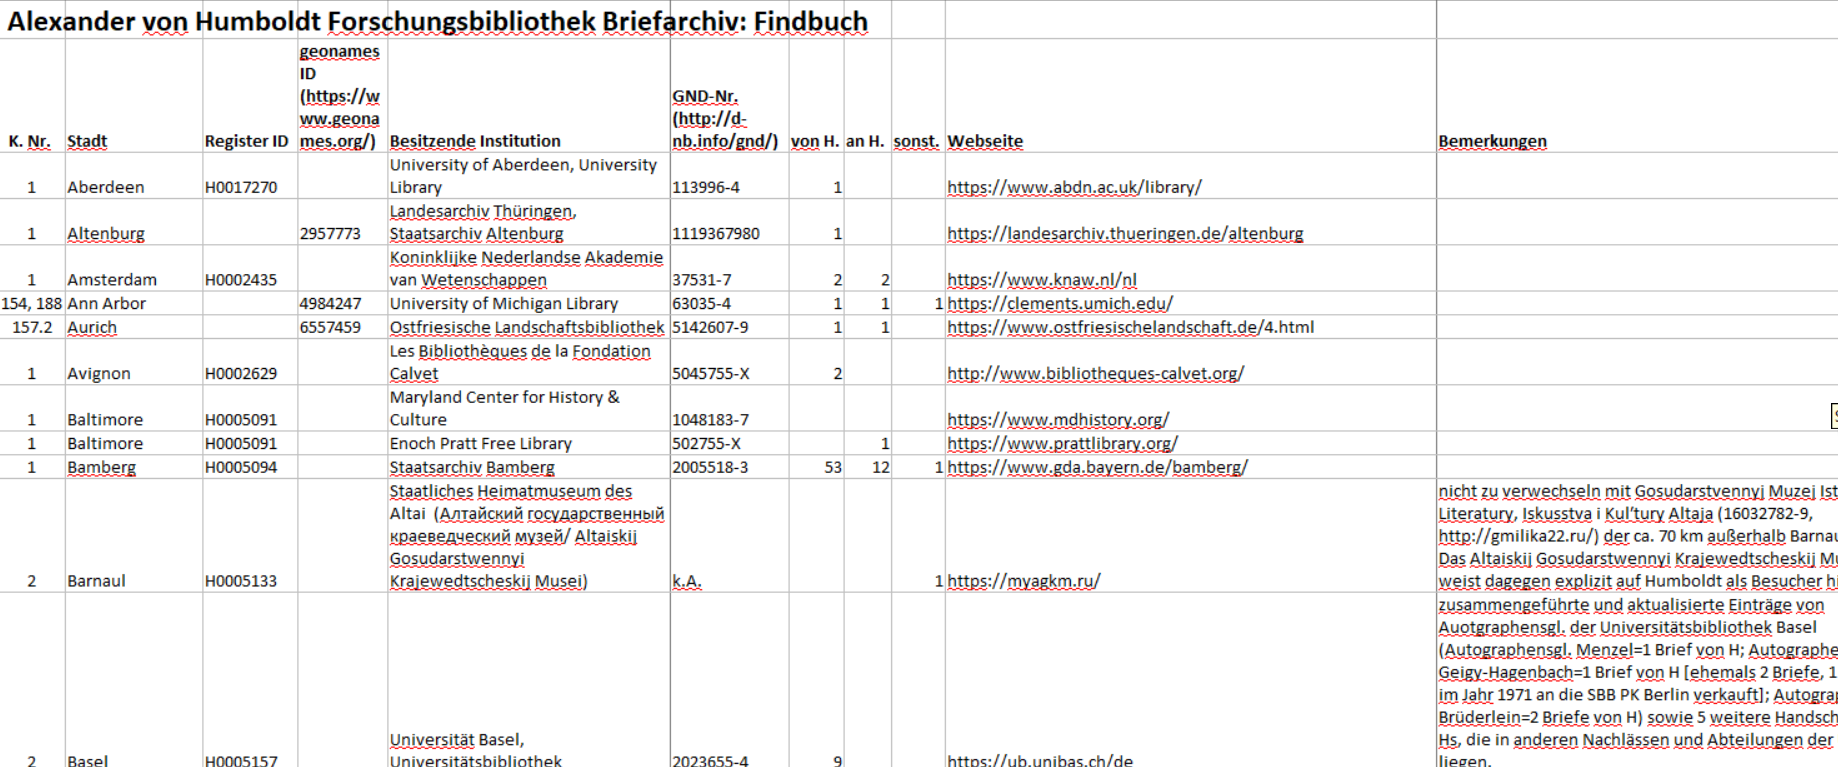
\includegraphics[scale=0.4]{img/findbuch_numérisée.png}
    \hfill
\end{figure}

Cette aide à la recherche a été entièrement retranscrit numériquement dans un tableau Excel par Anne MacKinney, ancienne stagiaire au sein du projet d'édition \textit{Alexander von Humboldt auf Reisen - Wissenschaft aus der Bewegung} en mars 2021. Ainsi, les données de l'aide à la recherche, à savoir côte du tiroir de classement, ville, institution propriétaire, détails des documents conservés, y sont retranscrits. En plus de ces données ont été rajoutés l'identifiant GeoName et l'identifiant interne à l'édition des lieux de conservation, le site internet de l'institution conservant les documents ainsi qu'une colonne commentaire. Si l'institution concernée a déposé ses données sur le site du Kalliope-Verbund\footnote{Voir la \autoref{sub:kalliope}.}, alors la requête a été copiée dans le document afin d'avoir un accès direct à la correspondance d'Alexander von Humboldt conservée dans cette institution-ci. 

Ce tableau a permis d'effectuer l'inventaire des documents conservés\footnote{Voir tableau présentant le nombre de documents d'archives d'Alexander von Humboldt conservés à la BBAW, \autoref{tab:tableauxDocsConservés}.} au sein de la \gls{bbaw}. En plus d'être le point de départ de la première mission de mon stage, il a également été utile pour l'outil expérimental développé par Dr. Gordon Fischer pour le projet \textit{Alexander von Humboldt auf Reisen}.


\section{\textit{Humboldt Chrotonopographie} : un outil expérimental}
\label{sect:chronotopographie}
En effet, les données de l'aide à la recherche ont été insérées au sein du projet \textit{Humboldt Chronotopographie}. Ce projet a pour but de visualiser grâce aux cartes les itinéraires empruntés lors des divers voyages et expéditions d'Alexander von Humboldt. Il a pour vocation de proposer des données ouvertes téléchargeables par tous et de devenir un projet collaboratif. Ce travail, à la croisée d'outil de travail scientifique et de visualisations presque tout public, a débuté à l'automne 2020. Il est appuyé par l'équipe du projet \textit{Alexander von Humboldt auf Reisen} et est développé par Dr. Gordon Fischer, ingénieur au sein du service \textit{The Electronic Life Of The Academy} (\gls{telota}) qui est le pôle des humanités numériques de la \gls{bbaw}.
\begin{figure}[h]
    \centering
    \caption{Copie d'écran générale de l'outil \textit{Humboldt Chronotopographie}}
    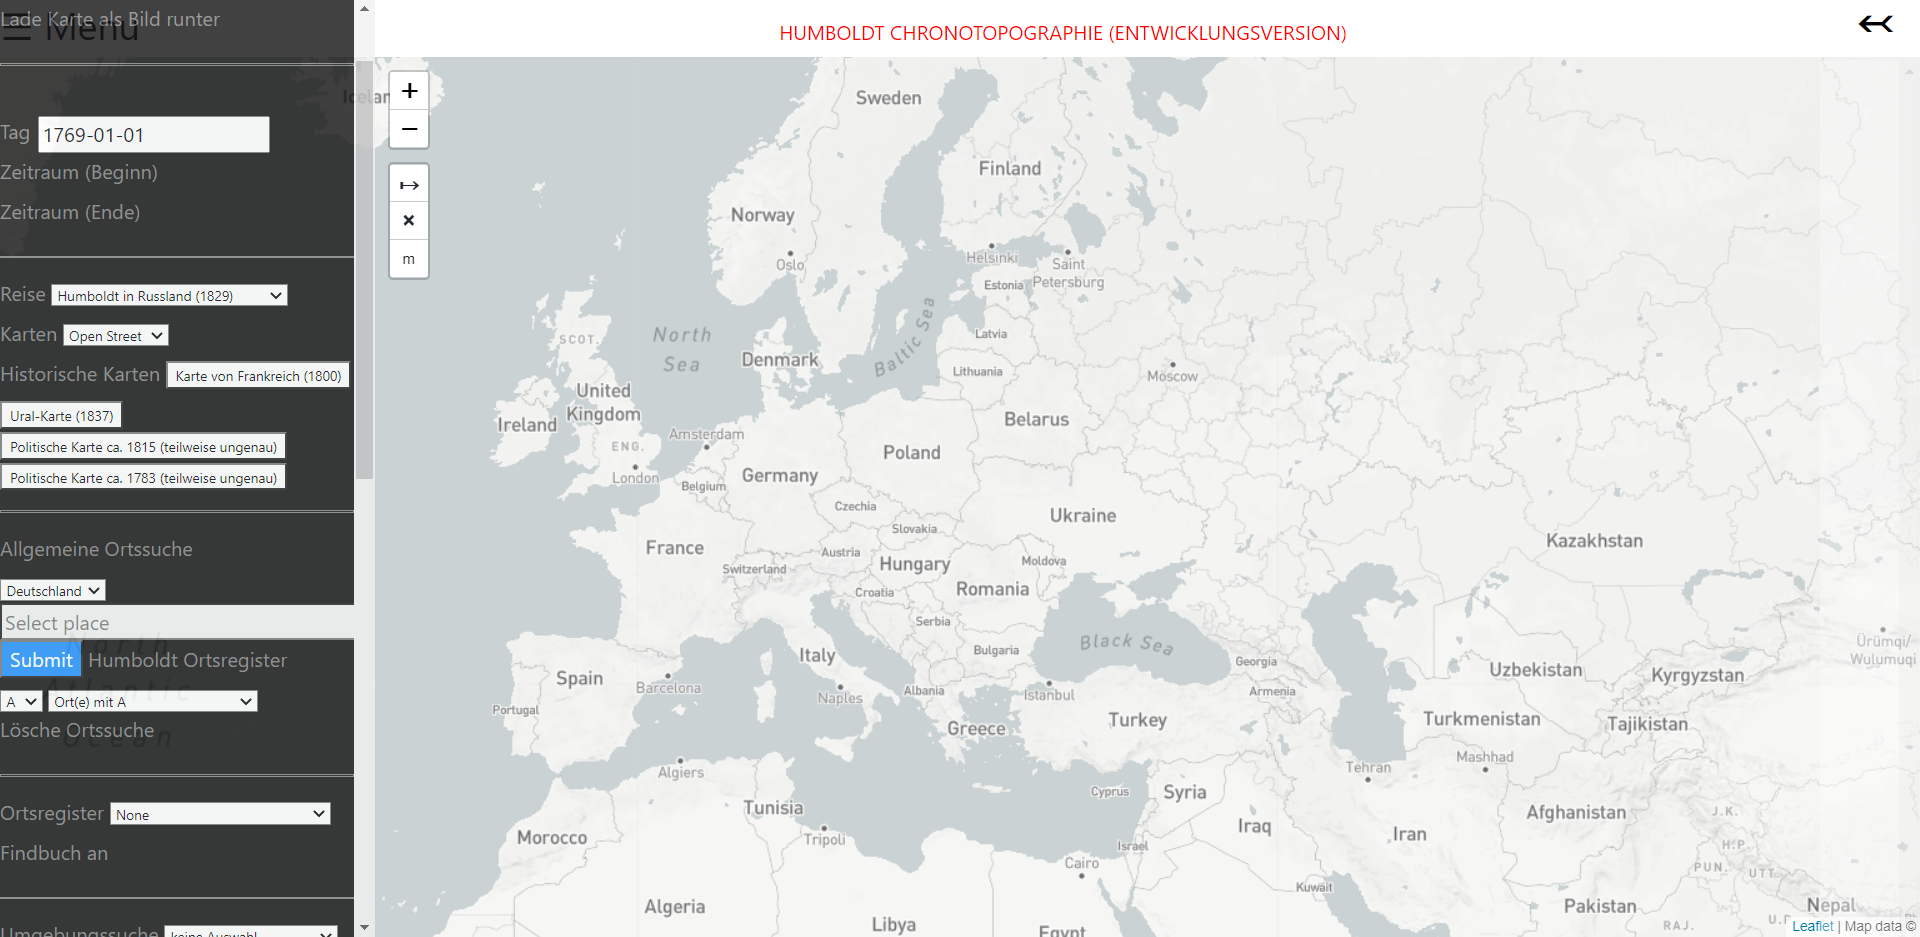
\includegraphics[scale=0.4]{img/chronotopographie/chrono_general.png}
    \hfill
\end{figure}

Le menu de gauche\footnote{cf \autoref{fig:chronoFindbuch}.} de cet outil permet de sélectionner ce que l'utilisateur souhaite visualiser : définir une période, choisir son fond de carte, choisir un voyage ou bien des données particulières. Dans ce menu, il suffit de cliquer sur \textit{Findbuch an} (en français : afficher le catalogue) afin de visualiser tous les lieux de conservation des documents manuscrits sur une carte du monde. Un menu à droite s'affiche alors avec la ville et l'institution conservatrice. Le détail des documents conservés au sein de l'institution est également affiché. Ces données forment une visualisation en elles-mêmes et ne sont pas reliées à d'autres données\footnote{Voir la copie d'écran de cette visualisation,  \autoref{fig:chronoFindbuch}.}. Les données ont directement été extraites du tableau Excel et ont été insérées dans l'outil expérimental au cours de son développement. 

Dans les premiers temps du développement de l'outil, l'accent a été mis sur les données chronotopographiques de l'\textit{edition humboldt digital}. Ces données sont la combinaison de la datation et la géolocalisation des informations provenant des carnets de voyage du scientifique. À noter que ces données sont elles-mêmes un ensemble de données reliées à des ressources externes\footnote{cf. \autoref{chap:édition et données tierces}}.

Les itinéraires de voyages de Humboldt, que ce soit la grande expédition américaine (1799-1804) ou encore l'expédition en Russie et Asie centrale entreprise en 1829, n'ont encore jamais été visualisées de manière dynamique. Dans l'édition numérique, chaque lieu qui a été balisé dans un \texttt{<placeName>} au sein de l'encodage \gls{xml} est relié à son identifiant GeoName et à son identifiant interne à l'édition\footnote{cf \autoref{sect:interEtLinkedData}.}. Environ 3000 lieux sont balisés dans un \texttt{<placeName>} au sein de l'\textit{edition humboldt digital}. Afin de visualiser les divers itinéraires de voyage de Humboldt, les données sont extraites directement des documents encodés en \gls{xml}-\gls{tei} de l'édition et plus particulièrement des registres de lieux et des entrées chronologiques. Ces données alors agrégées forment un nouvel ensemble de données exploitable par l'outil chronotopographique et stockées dans une base de données eXist-DB. Elles sont visualisables via une transformation \gls{xsl}t vers \gls{html} sur l'application web \textit{Humboldt Chronotopographie}.

\begin{figure}[h!]
    \centering
    \caption{Copies d'écran de \textit{Humboldt Chronotopographie}}
         \begin{subfigure}[b]{0.4\textwidth}
         \centering
         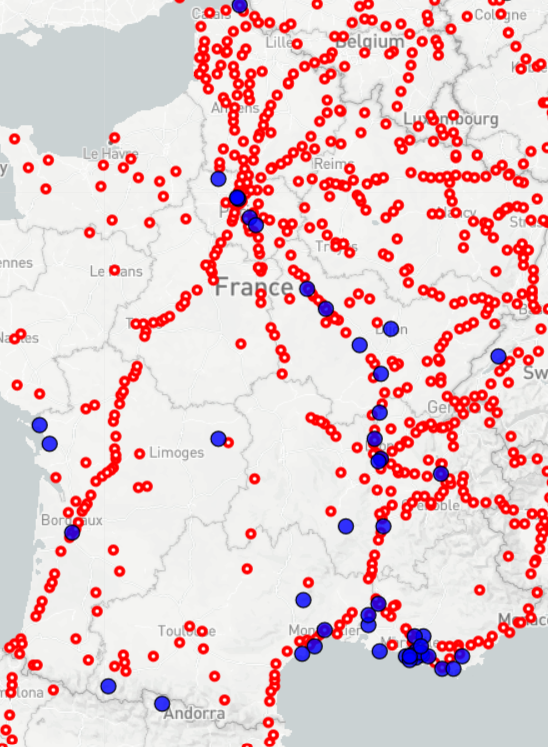
\includegraphics[height=1.4\textwidth]{img/chronotopographie/chrono_frankreich_poststationen.png}
         \caption{Itinéraire de Humboldt en France en 1798 (en bleu) superposé aux relais de poste (en rouge).}
        \end{subfigure}
        \hfill
        \begin{subfigure}[b]{0.4\textwidth}
         \centering
         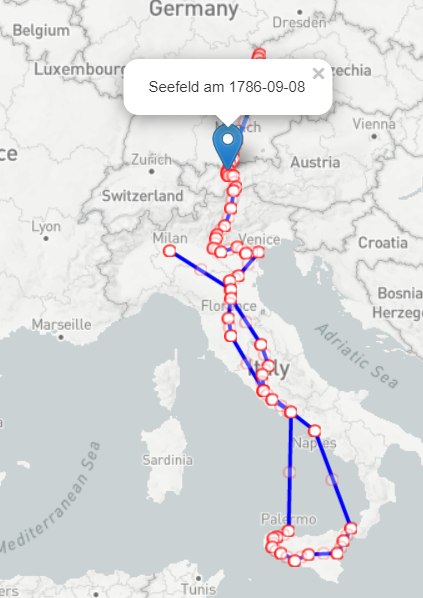
\includegraphics[height=1.4\textwidth]{img/chronotopographie/chronoto_reise_goethe.png}
         \caption{\href{https://telotawebdev.bbaw.de/avhr/reisetagebuecher?reise=goethe_italien&dist=90&days=500}{Animation de l'itinéraire de Goethe lors de son voyage en Italie en 1786}.}
        \end{subfigure}
\end{figure}

L'un des objectifs de cet outil expérimental est donc de visualiser les voyages et lieux de séjour d'Alexander von Humboldt en exploitant les données de l'\textit{edition humboldt digital}, enrichies par des données tierces et en les liant à des services web divers. Les données du projet ont été complétées par des donnés externes comme les routes postales définies par Giacomo Casanova. Toutes les villes possédant un relais postal sont listées et sont accessibles de manière ouverte sur le site de \href{https://giacomo-casanova.de/posten.htm}{giacomo-casanova.de}. Dr. Gordon Fischer a, pour chaque lieu listé, ajouté sa géolocalisation et son identifiant GeoName. Il est ainsi possible de faire apparaître tous les relais de poste listés par Casanova vers 1750 et de les comparer avec les routes empruntées par Humboldt lors de ses itinéraires comme le présente la capture d'écran (a) ci-dessous. Humboldt a donc suivi une des routes principales où les relais de poste sont particulièrement nombreux afin de descendre de Paris vers le sud de la France. 
Dans l'avenir, il s'agirait de pouvoir visualiser les routes de voyages empruntés par d'autres figures de l'histoire contemporaine. Un voyage en Italie effectué par Goethe en 1786 a d'ailleurs été pris en exemple et inséré au sein de l'outil chronotopographique, comme le présente la copie d'écran (b) ci-dessus. 

Représenter les itinéraires de voyage n'est pas une idée inédite. En effet, il existe déjà divers projets d'humanités numériques qui proposent de visualiser les routes de voyage ou les voyages entrepris de certaines grandes figures lettrées de l'époque des Lumières. \textit{Mapping of the Republic of letters\footnote{Les visualisations et plus d'informations sont disponibles sur le \href{http://republicofletters.stanford.edu/}{site internet.}}}, développé à l'université de Stanford, propose de cartographier la République des Lettres avec notamment des visualisations sophistiquées et interactives de données sur les réseaux de correspondances et des cartes d'itinéraires de voyages de ces érudits de l'époque contemporaine. Il est ainsi possible de découvrir le réseau de correspondances de \href{http://republicofletters.stanford.edu/casestudies/voltaire.html}{Voltaire}, \href{http://republicofletters.stanford.edu/casestudies/condorcet.html}{Condorcet}, \href{http://republicofletters.stanford.edu/casestudies/franklin.html}{Benjamin Franklin} mais aussi des \href{http://republicofletters.stanford.edu/casestudies/grandtour.html}{voyageurs effectuant ce qu'on appelle le Grand Tour\footnote{Le Grand Tour, aussi appelé \textit{Junkerfahrt} ou \textit{Cavaliertour} dans les pays du Saint-Empire romain germanique, avaient diverses fonctions éducatrices : approfondir ses connaissances dans les arts et sciences sociales, acquérir une formation politique approfondie avec notamment la comparaison des systèmes politiques des lieux visités, rencontrer des jeunes aristocrates étrangers ou du moins vivant à l'étranger. Ces voyages avaient une fonction sociale une fois que les jeunes aristocrates rentraient au pays puisqu'ils constituaient un élément de reconnaissance ou d'ascension sociale en affirmant les moyens financiers et la culture du jeune aristocrate. Alexander von Humboldt a effectué un tour d'Italie avec Gay-Lussac quelques mois après son expédition en Amérique du sud en 1805. L'historienne, Marie-Noëlle Bourguet, revient sur ce voyage de plusieurs mois en analysant notamment le carnet de voyage du scientifique, voir \cite{bourguet_monde_2017}.}}. Une visualisation cartographique des villes italiennes visitées par des architectes au cours de leur Grand Tour permet de rendre compte des villes les plus visitées au cours du XVIII\textsuperscript{e} siècle. Chaque point expose le nom du lieu et le nombre d'architectes qui l'ont visité. La taille du point représenté est proportionnelle au nombre de visites du lieu. Par ailleurs, le site \href{https://ernie.uva.nl/}{\gls{ernie}} est un site collaboratif, proposant des données ouvertes de plus de 1700 articles analytiques sur divers thèmes et figures emblématiques de cette époque. Il se propose de retracer la montée internationale de la construction de la culture nationale dans l'Europe du XIX\textsuperscript{e} siècle, construction qui s'est établie au sein du mouvement romantique-nationaliste\footnote{Voir la \href{https://ernie.uva.nl/viewer.p/21/56}{documentation du site}.} à travers tout matériel produit à cette époque à savoir les lettres, la musique, les oeuvres peintes, mais aussi d'autres événements comme les expositions ou les voyages individuels. Cette plateforme d'études académiques destinée à l'étude critique des documents historiques est un projet collaboratif avec la participation de plus de 361 contributeurs principalement situés en Europe et en Amérique du Nord\footnote{Voir la \href{https://ernie.uva.nl/viewer.p/21/68/scenario/125/geo}{carte du monde des contributeurs}.}. \gls{ernie} propose à ses utilisateurs de visualiser une quinzaine d'itinéraires de voyage. Tous apparaissent sur une même carte et le menu de droite contenant la liste des itinéraires disponibles permet de désélectionner ceux que l'utilisateur ne souhaite pas visualiser. Cliquer sur un point apparaissant sur la carte permet d'avoir accès à des informations supplémentaires dont notamment le site internet du projet collaborateur.
\begin{figure}[h!]
\centering
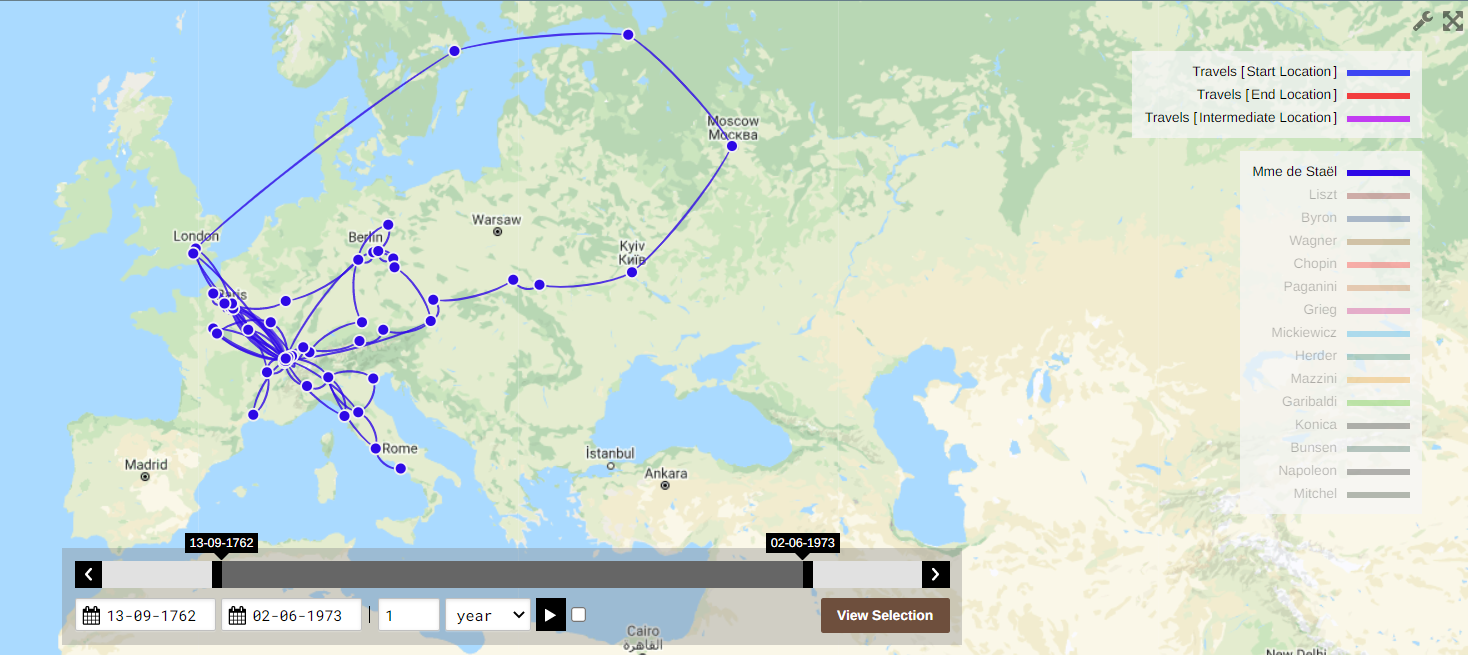
\includegraphics[scale=0.5]{img/ernie_stael.png}
\caption{Copie d'écran du site ERNIE présentant l'itinéaire du voyage de Mme de Stäel, itinéraire sélectionné dans le menu à droite.}
\end{figure}

À la différence de tous ces autres projets d'humanités numériques, l'outil développé par la \gls{bbaw} a pour vocation, en plus de présenter les données de l'édition, d'accompagner les chercheurs dans leur recherche scientifique et de combler les lacunes des données. En effet, dans ses carnets de voyage, Humboldt n'a pas toujours précisé toutes les villes-étapes où il a séjourné. Par conséquent, il existe des lacunes de plusieurs jours dans ses itinéraires.

\begin{figure}[h!]
\centering
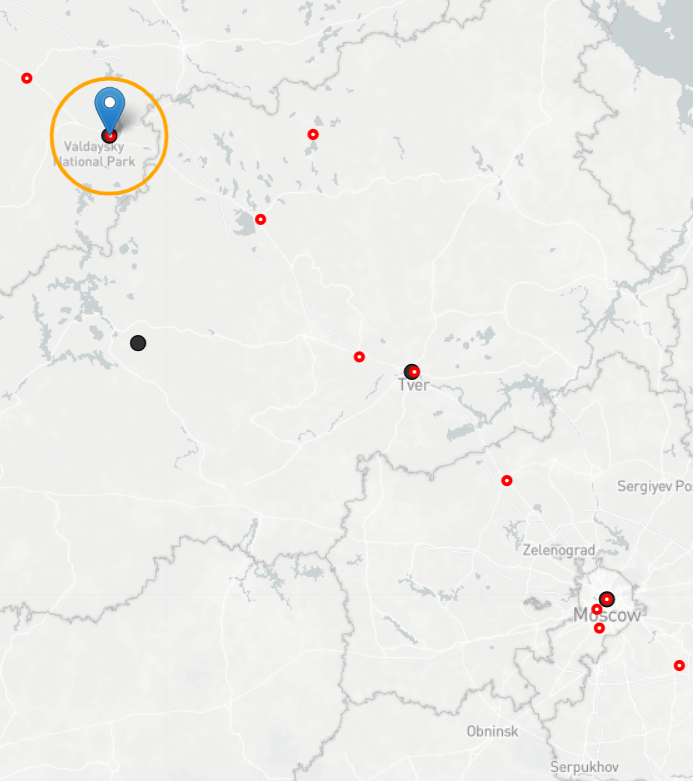
\includegraphics[scale=0.5]{img/chronotopographie/chrono_valdai_moscou.png}
\caption{Définir un itinéraire : l'exemple de Valtaï à Moscou}
\end{figure}
\newpage
Prenons l'exemple, représenté ci-dessus, d'un itinéraire effectué lors du voyage en Russie et Asie centrale de 1829. Humboldt écrit dans son journal "\textit{De Pét à Moscou 113–27 (Waldai II 59)}\footnote{\textit{Fragmente des Sibirischen Reise-Journals 1829}, 9r. L'édition de cette page accompagnée de son facsimilé est disponible dans l'\textit{\href{https://edition-humboldt.de/reisetagebuecher/detail.xql?id=H0005449&view=f&l=de&page=9r}{edition humboldt digital}}.}". Il va donc de Saint-Pétersbourg à Moscou en passant par la ville de Valdaï. Cependant, quelles ont été les étapes entre toutes ces villes ? Moscou se situe à plus de cinq jours de voyage de la ville de Valdaï. Grâce à l'outil développé, il est possible de choisir une zone de recherche à savoir entre un et cinq jours de voyage. En cliquant sur un lieu, une zone s'affiche sous forme de cercle à partir du lieu sélectionné et permet au chercheur de définir les possibles lieux de séjour de Humboldt. En croisant ces données avec les relais de poste listés par Casanova et intégrés à l'outil, il est également possible de définir les routes les plus empruntées et ainsi d'émettre des hypothèses quant aux lieux où Humboldt a pu séjourner. Sur la copie d'écran, le cercle orange représente la zone autour de la ville de Valdaï accessible en un jour de voyage. À savoir qu'un jour de voyage en cheval a été estimé à une trentaine de kilomètres. C'est en tous cas l'estimation utilisée dans l'outil \textit{Humboldt Chronotopographie} afin d'établir ces zones. Les points rouges représentent les relais de poste appartenant à la liste de Casanova et les points noirs sont les villes évoquées par Humboldt dans son carnet de voyage. L'évocation d'une ville ou d'un lieu ne signifie pas que Humboldt y a séjourné. Il n'existe aucune différence dans l'encodage pour les villes où Humboldt a séjourné et celles dont il fait une simple référence. Par conséquent et puisque les données représentées dans l'outil sont directement issues de l'encodage, l'outil ne peut effectuer une différence dans l'affichage de ces points qui sont alors représentés de la même manière.

\begin{wrapfigure}{r}{0.5\textwidth}
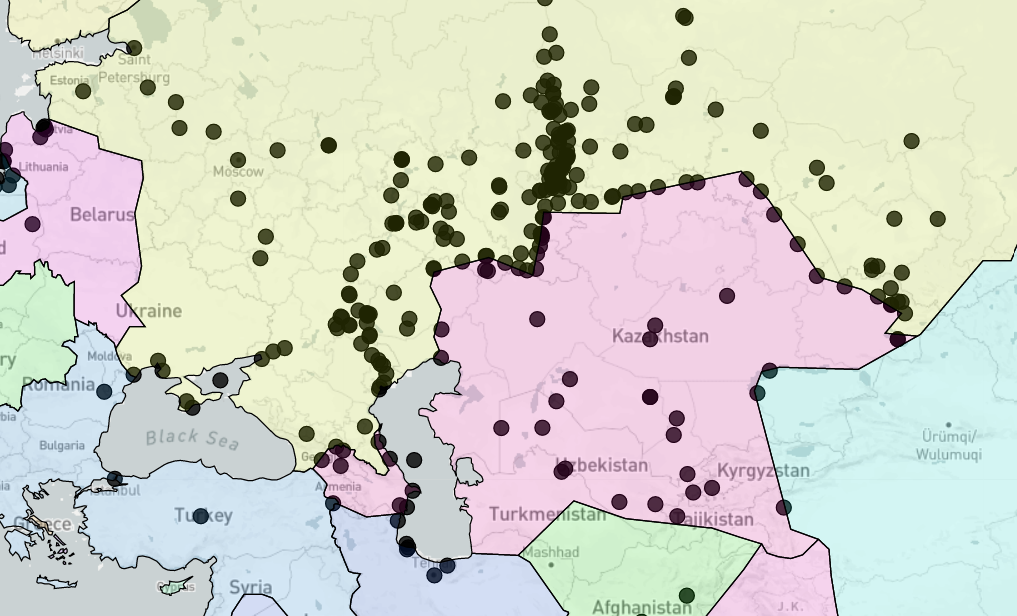
\includegraphics[width=0.5\textwidth]{img/chronotopographie/chrono_kazakhstan.png}
\caption{Superposer les cartes : exemple de la frontière kazakhe}
\end{wrapfigure}
L'outil permet également de superposer divers fonds de cartes qui apportent des informations supplémentaires à l'utilisateur. Trois fonds de cartes additionnels sont disponibles sur \textit{Humboldt Chronotopographie} : la carte mondiale des frontières politiques vers 1783 et celle vers 1815 ainsi qu'une carte de la France vers 1800\footnote{Voir les différents fonds de cartes,  \autoref{fig:fondsCartes}}. Les lieux tirés des carnets de voyage de Humboldt se superposent au fond de carte choisi. Il est ainsi plus aisé de situer les itinéraires entrepris par le scientifique. Cela a permis de remarquer par exemple que Humboldt a suivit la frontière kazakhe lors de son voyage en Russie et en Asie centrale de 1829, comme le présente la carte ci-contre. 


\chapter{Développement d'outils de recherche et des visualisations}
\label{chap:rechercheEtViz}
\chaptermark{Fonctions de recherche et visualisations}
Dans les traces de l'outil \textit{Humboldt Chronotopographie}, ma première mission de stage a été de reconstruire, du moins en partie, la correspondance d'Alexander von Humboldt et de proposer des fonctions de recherche afin de l'explorer. Le développement de ces fonctions a été soutenu techniquement par Dr. Gordon Fischer, ingénieur au sein du pôle \gls{telota} de la \gls{bbaw} et développeur de l'outil expérimental \textit{Humboldt Chronotopographie} sur les carnets de voyages d'Alexander von Humboldt pour le projet \textit{Alexander von Humboldt auf Reisen}. Dr. Ulrich Pässler, chercheur et responsable du projet de recherche et d'édition ainsi que tuteur de mon stage, en a supervisé la conception. 

Numériser toutes les photocopies conservées au sein des archives Humboldt de la \gls{bbaw} est un travail de plusieurs années. Afin de reconstruire de manière numérique les archives de la correspondance d'Alexander von Humboldt, il a été choisi, à partir de l'aide à la recherche retranscrit numériquement, d'aller chercher les données correspondantes aux lettres manuscrites écrites et reçues par Alexander von Humboldt directement sur les sites d'archives conservatrices de ces lettres proposant des données accessibles. 
Les données utilisées au sein de ce projet proviennent du Kalliope-Verbund\footnote{Voir la \autoref{sub:kalliope}.}, du Catalogue général de la Bibliothèque nationale de France\footnote{Voir la \autoref{sub:BNF}} et de la Société américaine de philosophie\footnote{Voir la \autoref{sub:APS}.}. Afin d'explorer et de découvrir les données de cette nouvelle collection numérique de la correspondance de Humboldt, des fonctions de recherche ainsi que des visualisations de données ont été réalisées.

\section{L'environnement technique et les librairies choisis}
Les visualisations de données constituent un moyen d'expression modulable afin d'exposer les données de la correspondance d'Alexander von Humboldt. Visualiser sur une carte les échanges épistolaires de ce dernier permet de rendre compte de l'ampleur de ceux-ci et du réseau mondial dans lequel s'insère le scientifique.

\subsection{Le choix de l'environnement technique : Jupyter Notebook}
Il existe de nombreuses technologies qui permettent la réalisation de visualisations de données. Néanmoins, ces technologies ne sont pas toutes adaptées et n'exigent pas le même niveau de compétence technique. L'environnement technique dans lequel le projet se développe est également important pour la conception des visualisations : une visualisation sera différemment présentée sur une application Android ou sur une application web, de même, si elle a pour vocation d'être interactive ou statique. L'environnement technique choisi présente des configurations réduites aux fonctionnalités qu'il propose. Ces possibilités de configuration ont un impact direct sur les réalisations potentielles. 

Le choix de l'environnement technique dans lequel ont été développées les fonctions de recherche et les visualisations s'est porté sur les Jupyter Notebook. Il s'agit d'une application web et open-source qui permet de créer des documents compartimenté par cellule. Chacune d'entre elle peut avoir une typologie de contenu différente telle que du code ou du Markdown. Cela permet au programmeur de documenter de manière riche ses cellules de code. Ces dernières peuvent être lancées indépendamment des unes des autres ce qui est un réel avantage afin de pouvoir tester quelques lignes de code ou une unique fonction par exemple. 

Les Jupyter Notebook présentent de nombreux avantages : 
\begin{itemize}
    \item Ils proposent des sorties de cellule, appelés \textit{outputs}, interactifs avec l'utilisation possible de \gls{html} mais aussi l'affichage d'images et de visualisations interactives.
    \item Ils supportent plus de quarante langages de programmation différents.
    \item Ils permettent d'exploiter et d'explorer les données à l'aide de nombreux outils et librairies utilisables directement en leur sein. 
\end{itemize}

Les utilisations possibles des Jupyter Notebook sont multiples : le nettoyage et la transformation des données, la modélisation statistique, la visualisation des données, le machine learning... En effet, les Jupyter Notebook sont particulièrement puissants dans le traitement de données et notamment de larges sets de données. Dr. Gordon Fischer a notamment utilisé des Jupyter Notebook afin d'extraire des données affichées sur l'application web \textit{Humboldt Chronotopographie}\footnote{cf \autoref{sect:chronotopographie}.}.

Un des avantages des Jupyter Notebook est le fait qu'il n'y ait pas besoin de programmer une application web complète pour visualiser des données. Néanmoins, il faut avoir quelques connaissances techniques afin de pouvoir utiliser un Jupyter Notebook : ce n'est en effet pas un outil grand public. Si on souhaite que le grand public ait accès aux données et au projet alors il serait plus judicieux de développer une application web à laquelle les utilisateurs auraient directement accès par leur moteur de recherche. Sans être un projet à part entière, l'utilisation des Notebooks peut également être une étape au sein de la conception d'un site internet en rendant compte des données et des visualisations qui y seraient proposées.

\subsection{Les librairies utilisées}

Les Notebooks supportent de nombreux widgets interactifs qui permettent aux utilisateurs de visualiser et contrôler les changements au sein de leurs données. Ces widgets sont proposés par diverses librairies. Certaines d'entre elles ont été nécessaires pour le développement de fonction de recherche et de visualisations. Toutes les librairies qui ont été utilisées pour leur élaboration sont open source.

\subsubsection{Ipyleaflet}
Ipyleaflet permet de créer des cartes interactives au sein des Jupyter Notebooks. Cette librairie prend en charge les annotations, les divers marqueurs de lieux et propose différents fonds de cartes.
Elle est particulièrement adaptée afin de réaliser des visualisations cartographiques de la correspondance d'Alexander von Humboldt.

La documentation est bien fournie sur le site qui lui est dédié\footnote{Voir le site \href{https://ipyleaflet.readthedocs.io/}{ipyleaflet.readthedocs.io}}. Chaque fonctionnalité de la librairie est présentée avec des exemples de code afin de la prendre en main aisément. 

\subsubsection{Ipywidgets}
Ipywidget est également connu sous le nom de jupyter-widgets. Cette librairie propose de nombreux widgets \gls{html} interactifs au sein des outputs de cellules d'un Jupyter Notebook. 
Un widgets est un objet du langage de programmation, ici Python. Ils ont une représentation dans le navigateur web de l'utilisateur. Ils servent notamment à créer des interfaces graphiques interactives. 
La librairie met à disposition environ une quinzaine de widgets et fournit pour chacun une documentation explicite\footnote{Voir la documentation sur \href{https://ipywidgets.readthedocs.io/}{ipywidgets.readthedocs.io}}. Le programmeur peut avoir la parfaite maîtrise de l'apparence des widgets grâce aux nombreux paramètres disponibles pour chacun d'entre eux. 

\subsubsection{Pandas}
Pandas est une librairie proposant des outils d'analyse et de manipulation de données. Elle est particulièrement adaptée pour les structures de données. Parmi elles, DataFrame est une des principales structures de données gérées par cette librairie. Il s'agit d'un stockage des données en deux dimensions, c'est-à-dire sous forme de tableau. Cette structure de donnée a régulièrement été utilisée au sein de notre projet notamment pour présenter les résultats des fonctions de recherche. 

\begin{figure}[h!]
\centering
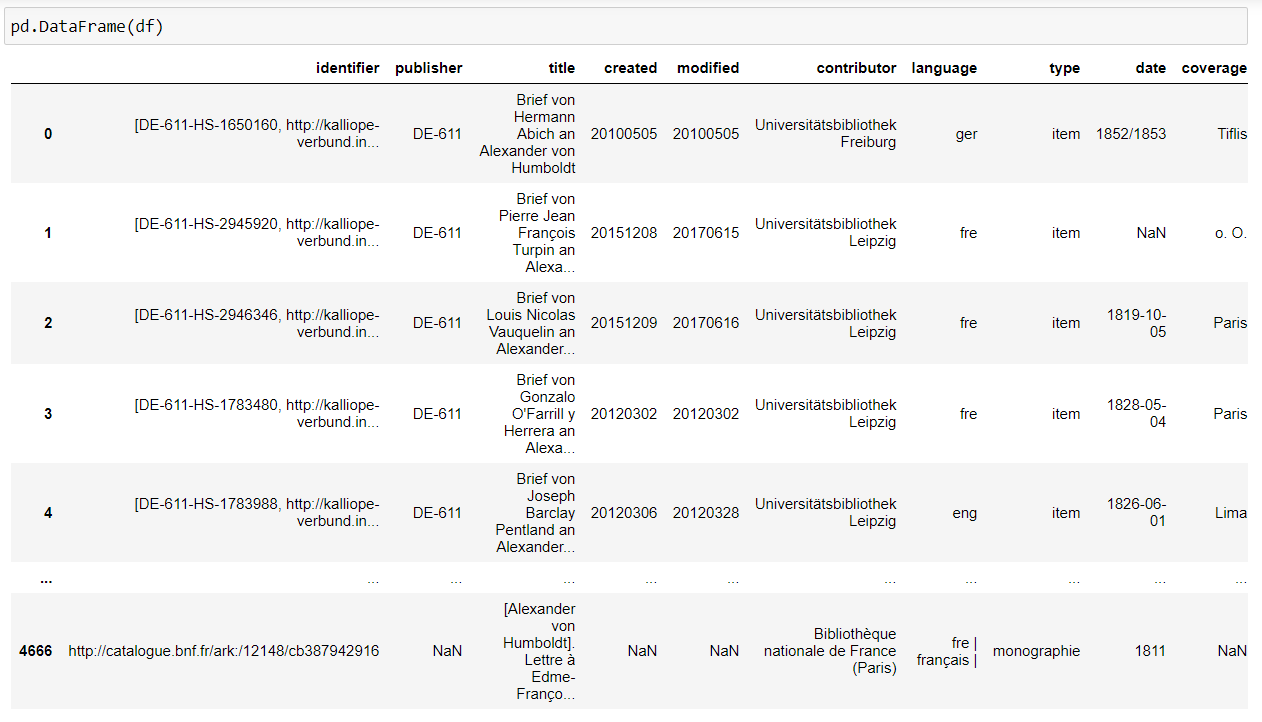
\includegraphics[scale=0.5]{img/dataFrameAllData.png}
\caption{Structure de données de la librairie pandas : dataframe de toutes les données de la correspondance d'Alexander von Humboldt}
\label{fig:DataFrame}
\end{figure}

\begin{wrapfigure}{r}{0.6\textwidth}
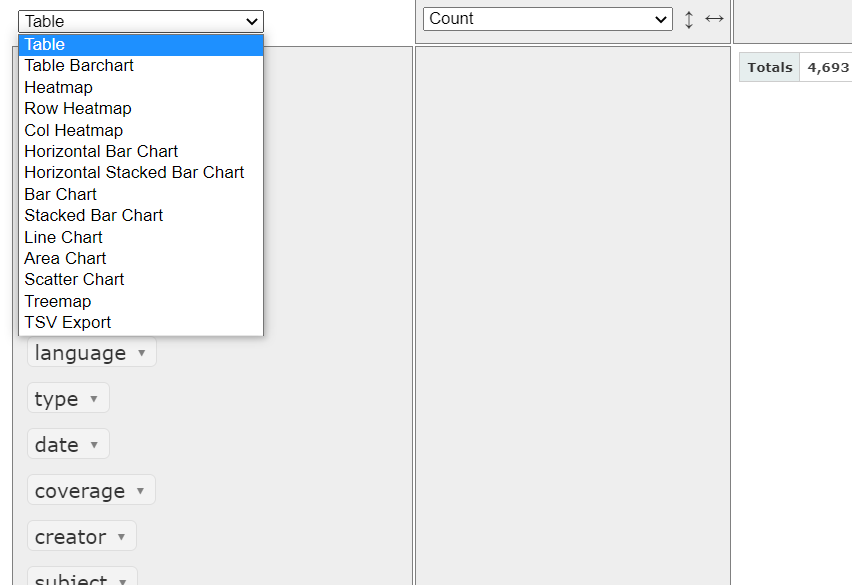
\includegraphics[width=0.6\textwidth]{img/pivot.png}
\caption{Table pivot de pandas avec toutes les données de la correspondance d'Alexander von Humboldt}
\vspace{-10pt}
\end{wrapfigure}

Pandas\footnote{La documentation est disponible sur \href{https://pandas.pydata.org/}{pandas.pydata.org}} propose également des fonctionnalités multiples dont la table pivot qui est un tableau croisé dynamique. La table pivot regroupe les données selon un ou plusieurs critères et les présente sous forme de sommes, de moyennes ou encore de comptage. Cette fonctionnalité se présente dans l'output d'une cellule d'un Jupyter Notebook et permet de manipuler les données de manière confortable et de les croiser. Une table pivot de la librairie pandas se présente comme ci-contre. Les données sont disponibles dans la colonne de gauche et sont manipulables au sein de l'output. En fonction de ce que l'on souhaite, il suffit de faire glisser les données de la colonne de gauche vers celle de droite ou sur la ligne du haut. La table pivot produit elle-même le calcul et présente les résultats sous forme de tableau.

\subsubsection{Matplotlib et NumPy}
Matplotlib est une librairie destinée à tracer et visualiser des données sous forme de graphiques. La documentation de matplotlib \footnote{Voir la documentation sur \href{https://matplotlib.org/stable/contents.html}{Matplotlib.org}} est particulièrement riche et détaillée. Toutes les possibilités de réalisation ou presque sont présentées et accompagnées de visuels afin de les prendre en main. 

Matplotlib est régulièrement combinée avec la librairie NumPy qui sert à effectuer des calculs scientifiques. Ces deux librairies forment un combo complet afin de réaliser des graphiques les plus complexes et avoir la totale maîtrise de leur apparence. 

\section{Algorithmie et réalisations}
L'algorithmie du projet a été rédigée en Python au sein de Jupyter Notebook. Les visualisations et les fonctions de recherche sont disponibles dans les cellules de sortie de ces documents une fois que les cellules de code ont été lancées. Un premier Jupyter Notebook a été crée pour les fonctions de recherche puis un second pour les visualisations. Ils ont pour vocation d'être utilisés par l'équipe du projet d'\textit{Alexander von Humboldt auf der Reisen} dont beaucoup sont chercheurs. Pour cette raison, la plus grande partie du code est "cachée" dans des fichiers \texttt{.py}. Dans les Notebooks, seulement quelques lignes sont visibles dans les cellules de code permettant de lancer l'algorithme des fonctions de recherche et des visualisations. Un des avantages des documents Jupyter Notebook est le fait d'associer des cellules de code et des cellules Markdown, utile à la rédaction d'une documentation qui apporte des informations sur les données utilisées, la présentation des résultats, des chiffres à propos des données. Cela ajoute du contexte à l'utilisateur autour des sets de données et du travail réalisé.

Présentons quelques informations chiffrées autour du set de données afin de comprendre l'ampleur de celui-ci. Pour rappel\footnote{Voir \autoref{chap:brutesàtraitées}.}, les données sont stockées sous format JSON et contient 4932 entrées de lettres reçues ou envoyées par Alexander von Humboldt. Parmi elles, se sont pas moins de 580 personnes ou institutions ayant envoyé une lettre au scientifique et 570 personnes ayant reçu une lettre écrite de la main de ce dernier. En tout, 351 lieux d'envoi ou de réception sont enregistrés. Dans ce set de données, y sont présentes les lettres de soixante-douze institutions. En effet, soixante-dix institutions conservatrices de ces lettres ont déposé leurs données sur le Kalliope-Verbundkatalog. Ces institutions ne sont pas toutes localisées en Allemagne puisqu'il y a notamment la Bibliotheka Jagiellonska située à Krakow ou encore Has-Sifriya hal-Le'ummit située à Jérusalem, parmi d'autres. À ces plusieurs dizaines d'institutions s'ajoutent la Bibliothèque nationale de France et la Société américaine de philosophie pour lesquelles les données ont été récupérées via leur \gls{api} respectives\footnote{cf \autoref{sub:APS} et \autoref{sub:BNF}.}. 

\subsection{Fonctions de recherche} 
Certaines fonctions de recherche permettent de rechercher au sein des institutions conservatrices de lettres. Pour ces fonctions, les données issues de l'aide à la recherche numériquement retranscrit sont venues enrichir le set de données de la correspondance d'Alexander von Humboldt. Cela augmente le nombre d'institutions conservatrices à 310 institutions au lieu de soixante-dix. Ce chiffre important témoigne du travail qu'il reste à effectuer afin de reproduire la collection analogue des archives Humboldt de la \gls{bbaw}. Malgré les données récupérées sur les diverses \gls{api}, le nombre de lettres enregistrées au sein de notre base de données reste inférieur au nombre de lettres enregistrées dans les archives Humboldt : 10 905 lettres à l'inventaire de 2021\footnote{En effet, 8690 lettres écrites par Humboldt et 2215 reçues par ce dernier ont été inventoriées. Voir \autoref{tab:tableauxDocsConservés}} contre 4932 dans notre base de données.

Les fonctions de recherche effectuent des recherches au sein de divers éléments : expéditeurs, destinataires, lieu de réception ou d'envoi et institutions conservatrices. Pour chacune de ces fonctions un dropdown menu permet à l'utilisateur de sélectionner la valeur voulue. Ce dropdown menu est accompagn d'un bouton \textit{New search} donnant la possibilité à l'utilisateur à tout moment d'effectuer une nouvelle recherche en relançant la cellule du Notebook. La fonction qui crée le bouton et permet relancer la cellule quand celui-ci est cliqué par l'utilisateur se présente comme ci-dessous.
\begin{figure}[h!]
\begin{lstlisting}
def btn_new_search():
    """
    Create a new search button.
    :return: btn
    :rtype: button
    """
    # Create the button
    btn = createButton('New search', 'info')
    output = wgt.Output()

    def new_search(b):
        # This function clears the ouput of a jupyter cell
        with output : 
            display(Javascript('IPython.notebook.execute_cell()'))
    
    # When the button is clicked, then the output of the jupyter
    # cell will be clean.
    btn.on_click(new_search)
    return btn
\end{lstlisting}
\vspace{-25pt}
\end{figure}

\begin{wrapfigure}{l}{0.38\textwidth}
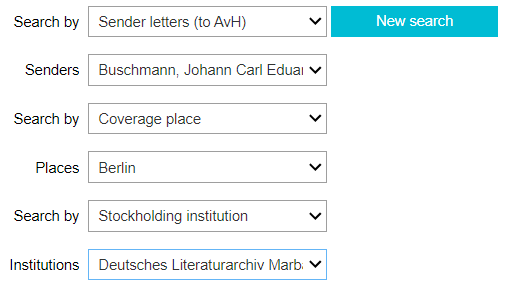
\includegraphics[width=0.38\textwidth]{img/recherche_dynamic.png}
\caption{Exemple des dropdown menus apparaissant de manière dynamique par la fonction récursive.}
\vspace{-10pt}
\end{wrapfigure}
Une fonction de recherche appelée dynamique a également été réalisée. Cette dernière autorise l'utilisateur à choisir dans un premier temps par quel élément de recherche il souhaite débuter son exploration et la fonction continue de proposer un nouvel élément de recherche jusqu'à ce qu'il n'y en ait plus ou bien jusqu'à ce que les résultats ne contiennent plus qu'une unique lettre. Ainsi, l'utilisateur peut tout d'abord sélectionner le nom d'un destinataire, puis l'année de la lettre, puis l'institution conservatrice de la lettre qu'il recherche, puis le destinataire jusqu'à ce que la lettre qu'il recherche apparaisse en tant que résultat. Cette recherche est possible par le développement d'une fonction récursive. Une fonction récursive est une fonction qui fait appel à soi-même au sein de son propre algorithme. Ainsi, notre fonction de recherche s'appelle soi-même et renvoie les éléments de recherches restants. En effet, l'utilisateur peut effectuer une recherche parmi quatre éléments, à savoir le destinataire, l'expéditeur, le lieu d'envoi et l'institution conservatrice. Si l'utilisateur choisit dans un premier temps le lieu d'envoi alors la fonction va effectuer un appel vers soi-même avec une liste des éléments de recherche restant, à savoir une liste contenant les éléments expéditeurs, destinataires et institutions de recherche. Le paramètre \textit{flag} est une variable booléenne qui permet à la fonction de reconnaître si c'est la première fois qu'elle est appelée ou bien s'il s'agit d'un appel récursif.

Toutefois, pour chacun des éléments énoncé ci-dessus à savoir les expéditeurs, les destinataires, le lieu de conservation et le lieu d'envoi des lettres, une fonction de recherche a été créée indépendamment des autres. Ainsi, l'utilisateur peut effectuer une recherche pour un élément précis sans avoir à utiliser la recherche dynamique. Chacune de ces fonctions de recherche indépendante des autres se présente sous deux éléments : un dropdown menu contenant les valeurs sélectionnables et un bouton \textit{New search}.


Prenons l'exemple de la création d'une fonction de recherche et notamment du dropdown menu pour la recherche à travers les dates. Afin de ne pas apporter trop d'informations à l'utilisateur mais aussi dans le but de réduire la quantité des valeurs sélectionnables, seules les années sont proposées au sein du dropdown menu et non toutes les dates entières sous le format YYYY-MM-DD. Afin de récupérer toutes les valeurs correspondantes aux dates de création au sein de la base de données \gls{json}, la fonction \texttt{nested\_lookup()} de la libraire \texttt{nested-lookup} effectue une recherche par clé sur un document. Cette fonction prend comme argument la clé recherchée au sein du document et le document dans lequel la fonction doit rechercher.  La fonction \texttt{nested\_lookup()} renvoie sous forme de liste les valeurs correspondantes à cette clé donnée. Cette liste retournée est ensuite nettoyée de différentes manières avant d'être envoyée, en tant qu'argument, à la fonction permettant de créer le dropdown menu.

\begin{wrapfigure}{r}{0.43\textwidth}
\vspace{-10pt}
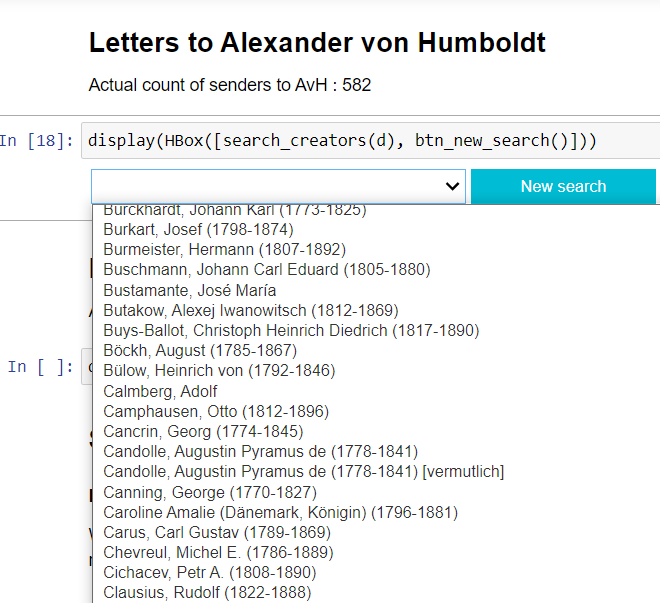
\includegraphics[width=0.43\textwidth]{img/recherche_dropdown.png}
\caption{Exemple du dropdown menu pour les expéditeurs de lettres.}
\vspace{-10pt}
\end{wrapfigure}
D'autre part, certaines lettres ont été rédigées par plusieurs personnes. C'est un cas fréquent notamment au sein de la famille Mendelssohn dont plusieurs membres sont en contact avec Humboldt. Cette famille rédige régulièrement des lettres à plusieurs. Tous les différents rédacteurs ont été encodés par les institutions conservatrice sous forme de tuples\footnote{Un tuple est un ensemble ordonné de valeurs. Le séparateur de chaque valeur est, en Python, une virgule.}. Pour les fonctions de recherche réalisées, il a été décidé de retirer ces tuples afin de proposer une liste plus claire de noms. C'est la fonction \texttt{avoidTupleInList()} qui retire ces tuples de la liste de noms. Ensuite, la fonction \texttt{getYears()} récupère pour chacune des dates les quatre premiers éléments de la date d'envoi, c'est-à-dire l'année. Une lettre au sein de la base de données se doit d'être envoyée ou reçue au cours des années de vie d'Alexander von Humboldt. Toutefois, des erreurs d'encodage sont présentes dans notre base de données. Au sein de celle-ci, certaines dates enregistrées en tant que date de création des documents se situent bien au delà de la date de naissance ou de décès du scientifique. On retrouve notamment 1937-02-18 pour une lettre d'Alexander von Humboldt à Johann Carl Eduard Buschmann\footnote{Buschmann est linguiste, bibliothécaire et est également le secrétaire privé des frères Humboldt. Il assiste également Alexander von Humboldt dans l'élaboration d'une de ses oeuvres principales \textit{Kosmos}. Par conséquent, les échanges épistolaires entre les deux hommes sont particulièrement riches comme le présente l'histogramme, \autoref{fig:histogrammeBuschmann}.} ou encore 1938-02-08 pour une lettre de Karl Degenhardt à Humboldt. Peut-être s'agit-il de copies des manuscrits. Afin d'éviter que ces éléments erronés apparaissent au sein de la liste du dropdown menu et qu'ils apportent de la confusion à l'utilisateur, ceux-ci sont retirés grâce à la fonction \texttt{getHumboldtYears()} qui retourne les lettres envoyées ou reçues entre 1769 et 1859. 
Ces explications faites, voyons à quoi ressemble à présent cette fonction qui permet de créer la fonction de recherche par date :

\begin{figure}[h!]
\begin{lstlisting}
def search_date(data:dict):
    """
    Create a dropdown menu with all years when a letter 
    (to and by AvH) has been sent
    :param data: dict 
    :return: dropdown menu
    :rtype: widget
    """
    years = getHumboldtYears(getYears(avoidTupleInList(nested_lookup('date', data))))
    dropdown = createDropdown('', years)
    dropdown.observe(onChangeDate)
    return dropdown
\end{lstlisting}
\vspace{-25pt}
\end{figure}

Une fois que la liste de valeurs est nettoyée et stockée dans la variable \texttt{years}, cette même-liste devient l'argument de la fonction qui crée le dropdown menu. La fonction \texttt{observe()}, quant à elle, gère l'accès aux données et leur présentation une fois qu'une valeur est sélectionnée par l'utilisateur au sein du dropdown menu. 

\subsection{Visualisations}
La façon dont l'utilisateur a accès aux données grâce aux visualisations sera abordée dans le chapitre prochain. Il s'agit ici de présenter la manière dont les visualisations ont été programmées et peuvent apparaître dans la cellule de sortie du Jupyter Notebook. 
Certaines visualisations sont directement liées aux fonctions de recherche, c'est-à-dire qu'elles sont le résultat d'une valeur sélectionnée dans un dropdown menu par l'utilisateur. En plus de la présentation des résultats par un DataFrame de la librairie pandas, les visualisations sont une autre représentation des résultats de recherche. Aussi, ces visualisations ne présentent qu'une partie, celle sélectionnée par l'utilisateur, des données de notre base de données.
Parmi ces visualisations, deux types sont à distinguer : 
\begin{itemize}
    \item les visualisations cartographiques. Ces dernières sont interactives c'est-à-dire que l'utilisateur peut zoomer, cliquer sur les différents points de la carte pour obtenir des informations supplémentaires.
    \item les visualisations représentant des histogrammes qui sont statiques.
\end{itemize}
\subsubsection{Les histogrammes}
Les histogrammes permettent de visualiser de manière graphique la répartition d'une variable. Cette répartition s'affiche sous forme de colonne. Les histogrammes sont particulièrement adaptés afin de représenter une variable dans la durée par exemple. Ces visualisations graphiques ont permis de représenter, au sein de notre projet, les échanges épistolaires entre une personne sélectionnée par l'utilisateur et Humboldt. 

Tout comme pour les fonctions de recherche, un dropdown menu est disponible afin que l'utilisateur sélectionne une personne. Ce menu est également accompagné d'un bouton \textit{New search}. Une fois qu'une valeur est choisie, l'histogramme des échanges de lettres apparaît.

\begin{wrapfigure}{r}{0.6\textwidth}
\vspace{-30pt}
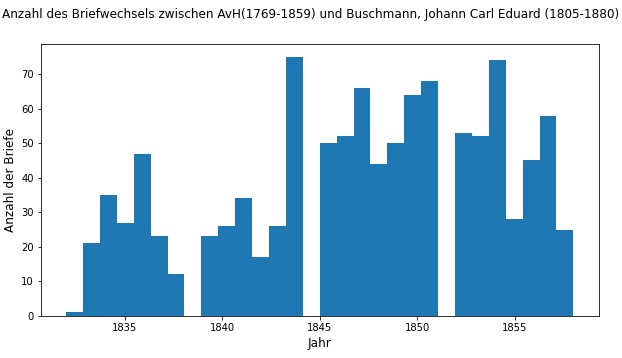
\includegraphics[width=0.6\textwidth]{img/birefwechselmitBuschmann.jpg}
\caption{Échanges épistolaires entre Buschmann et Humboldt}
\label{fig:histogrammeBuschmann}
\vspace{-47pt}
\end{wrapfigure}
Il est toutefois possible que rien ne s'affiche sur l'histogramme pour certains partenaires épistolaires. Cela signifie que pour toutes les lettres enregistrées dans la base et échangées entre cette personne et Humboldt aucune date n'est connue ou n'a été enregistrée par les catalogues en ligne sur lesquels les données ont été récupérées. Par conséquent, apparaissent seulement les lettres dont la date est connue. Afin d'avoir accès à toutes les données correspondantes à la personne sélectionnée, l'utilisateur est convié à se diriger vers les fonctions de recherche qui affichent toutes les données disponibles sans condition c'est-à-dire sous forme de DataFrame. Les visualisations des données sont par conséquent dépendantes des données enregistrées. Certaines de ces visualisations sont peu pertinentes quand les données sont incomplètes. Ce point mériterait des améliorations de code afin que l'histogramme s'affiche seulement quand il a des données à visualiser. 

\subsubsection{Les cartes}
De même que les histogrammes, les visualisations cartographiques sont dépendantes des données et plus particulièrement des données géographiques. Seulement les lettres accompagnées d'un lieu d'envoi ou de réception suffisamment précis et pour lesquelles les coordonnées correspondantes sont venues compléter notre set de données\footnote{Voir la partie \textbf{Enrichir} de \autoref{chap:brutesàtraitées}.} au moment de son enrichissement sont représentables. 

Bien que des visualisations cartographiques sont une représentation possible du résultat d'une fonction de recherche, deux cartes ont été créées afin d'exposer l'entièreté de la base de données\footnote{Voir les cartes \autoref{fig:allLettersMap} et \autoref{fig:allLettersMapColors}}. Ces cartes apportent une vue d'ensemble sur la correspondance de Humboldt. Grâce à elles, l'utilisateur peut prendre connaissance de l'ampleur de ces échanges épistolaires qui touchent tous les continents. En effet, à l'étude de ces cartes, il est devenu remarquable qu'au moins une lettre avait été reçue ou envoyée sur chacun des continents.

\begin{wrapfigure}{r}{0.43\textwidth}
\vspace{-25pt}
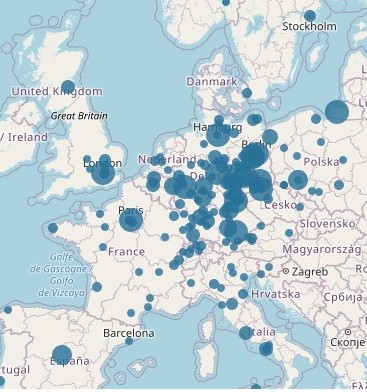
\includegraphics[width=0.43\textwidth]{img/mapviz_europe_extrait.jpg}
\caption{Zoom sur l'Europe de la carte représentant l'ensemble de la correspondance de Humboldt.}
\vspace{-15pt}
\end{wrapfigure}
La première de ces cartes expose tous les lieux où une lettre a été envoyée ou reçue par Alexander von Humboldt au cours de sa vie. Les points sur la carte sont des cercles dont la taille est proportionnelle au nombre de lettres reçues ou envoyées en ce lieu. En vérité, la taille des points n'est pas complètement proportionnelle pour des raisons de lisibilité. Pour chacun des lieux, le nombre de lettres envoyées ou reçues est calculé. Toutefois, si ce chiffre est supérieur à dix lettres alors le rayon du point sera de 12. Cela signifie qu'à partir de onze lettres, la taille du point représenté n'est plus proportionnel. Ces points, bien que non proportionnels au chiffre qu'ils représentent, sont malgré tout plus grands que ceux représentés proportionnellement permettant d'apporter un ordre de grandeur suffisant à l'utilisateur afin de comprendre l'information. Cela est important car si chaque rayon d'un point représenté restait proportionnelle au nombre de lettres qu'ils représente alors la carte deviendrait illisible. Prenons l'exemple de la ville de Berlin où 1134 lettres\footnote{Voir la carte, figure 6.2} y ont été reçues ou envoyées. Si le point représentant Berlin était proportionnelle à ces plus de milles lettres alors le point sera plus grand que la carte elle-même et elle deviendrait incompréhensible. L'opacité des points est de 80\% ce qui permet également une meilleure lisibilité de l'information puisque tous les points peuvent apparaître, même en transparence sous des points au rayon plus important et proches des uns des autres.

La seconde visualisations\footnote{Cette seconde carte est disponible dans les annexes, voir \autoref{fig:allLettersMapColors}} présente également toute la correspondance de Humboldt. Néanmoins, les points représentés ne sont pas proportionnels au nombre de lettres mais possèdent un code couleur. Ce code couleur est produit de manière aléatoire par l'algorithme et définit six grandes périodes dans la vie d'Alexander von Humboldt :
\begin{itemize}
    \item la période de ses études de 1792-1798
    \item le voyage en Amérique centrale de 1799 à 1804
    \item le voyage en Italie en 1805
    \item une période de sédentarisation parisienne de 1806 à 1828
    \item le voyage en Russie et Sibérie en 1829
    \item son retour à Berlin jusqu'à son décès de 1830 à 1859
\end{itemize}
Une légende rudimentaire informe du code couleur de chacune de ces périodes. Une explication ou du moins des informations supplémentaires pourraient accompagner cette légende afin d'apporter du contexte. Il serait également fort pratique que cette légende soit interactive : l'utilisateur cliquerait sur l'une des périodes permettant de faire disparaître les points des autres périodes de la carte. Cette fonctionnalité n'a pas été implémentée mais pourrait l'être si le développement d'une application web se concrétise. 

\begin{figure}[ht!]
\vspace{-15pt}
    \centering
         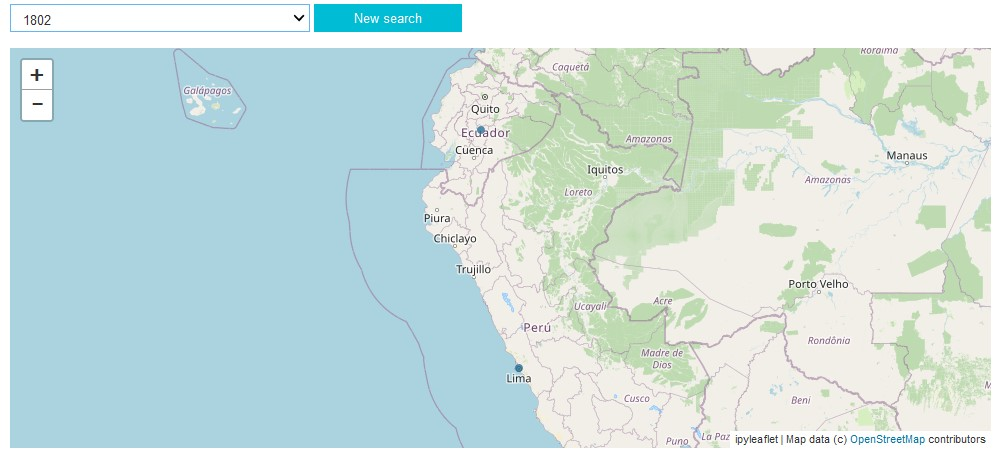
\includegraphics[scale=0.55]{img/mapviz_date_1802.jpg}
         \caption{Visualisation cartographique des résultats pour les lettres de l'année 1802 avec un zoom optimal.}
    \vspace{-15pt}
\end{figure}

Pour ce qui est des visualisations liées aux fonctions de recherche, elles se présentent sensiblement de la même manière que les deux visualisations expliquées précédemment. Toutefois seule une partie des données, celle sélectionnée par l'utilisateur, y est exposée. Un niveau de zoom optimal a été implémenté, c'est-à-dire que l'algorithme calcule le niveau de zoom le plus bas permettant d'afficher tous les points sur la carte. Cela apoorte une dynamique dans les cartes et améliore l'expérience utilisateur. Il serait malheureux d'afficher une mapmonde si un seul point est visualisé sur la carte.

Toutes ces cartes sont interactives : elles sont zoomables et cliquables. Cette interactivité permet à l'utilisateur d'avoir accès à des informations supplémentaires sur les données représentées : le nombre de lettres reçues ou envoyées en ce lieu, le nom du lieu, parfois le lien vers le catalogue en ligne quand il s'agit des visualisations liées aux fonctions de recherches. Malheureusement la taille d'affichage des visualisations cartographiques est contrainte par le format des Jupyter Notebook.

\let\cleardoublepage\clearpage


\chapter{Accessibilitées}
\label{chap:accessibilités}
Ce projet s'est construit au fil du temps, en adaptant les idées et besoins de l'équipe de \textit{Alexander von Humboldt auf der Reisen}. La conception du projet et des réalisations est loin d'avoir été linéaire. Le but premier était de reconstituer, du moins en partie, la collection analogue de photocopies des manuscrits issus de la correspondance du scientifique conservées au sein des archives Humboldt à la \gls{bbaw}. Les données concernant la correspondance d'Alexander von Humboldt ont été récupérées sur diverses \gls{api} conservatrices de lettres \footnote{Voir la \autoref{sect:donnéesStage}.}.
Ce projet a permis à ce que l'équipe de chercheurs (re)découvrent ces archives grâce aux nouvelles technologies qui leur sont, pour certains, peu familières. Cela a apporté des réflexions nouvelles sur des perspectives pour l'exploration de ces archives. Ce projet, à vocation originellement expérimentale, pourrait devenir une étape au sein d'une réalisation plus large : la conception d'une application web permettant aux chercheurs et autres utilisateurs de découvrir et d'étudier la correspondance du scientifique.

Bien que l'exploration des données de la correspondance ne soit pas disponible sur une application web entièrement grand public et accessible via un moteur de recherche, il est important que le projet jusqu'alors mené soit disponible sur une plateforme accessible afin que tous puissent avoir accès aux données qu'il contient. 

\section{Accès aux données}
La cellule de sortie affiche les différentes visualisations créées ainsi que les résultats des fonctions de recherche de diverses manières. Si une seule lettre est présente dans les résultats de recherche alors la page web du catalogue de l'institution conservatrice s'affiche dans l'output. L'avantage de présenter directement cette page au sein du Jupyter Notebook estd'apporter un accès direct à l'utilisation de toutes les informations concernant la lettre ainsi qu'à sa numérisation quand celle-ci est disponible. Dans la base de données, aucun lien vers la numérisation du document n'est stocké. C'est pour cela que l'accès à la page web du catalogue est intéressante. Toutefois, cette représentation de la page web n'est plus possible quand le résultat de la recherche contient plusieurs lettres. Dans ce cas, les résultats s'affichent sous forme de DataFrame de la librairie Pandas\footnote{Voir \autoref{fig:DataFrame}.} permettant à l'utilisateur d'avoir une vue d'ensemble de toutes les informations stockées pour les lettres résultantes. 

\begin{changemargin}{-1.5cm}{-1cm}
\begin{figure}
    \centering
    \caption{Accès aux catalogues en ligne. }
    \begin{subfigure}[b]{0.6\textwidth}
        \centering
        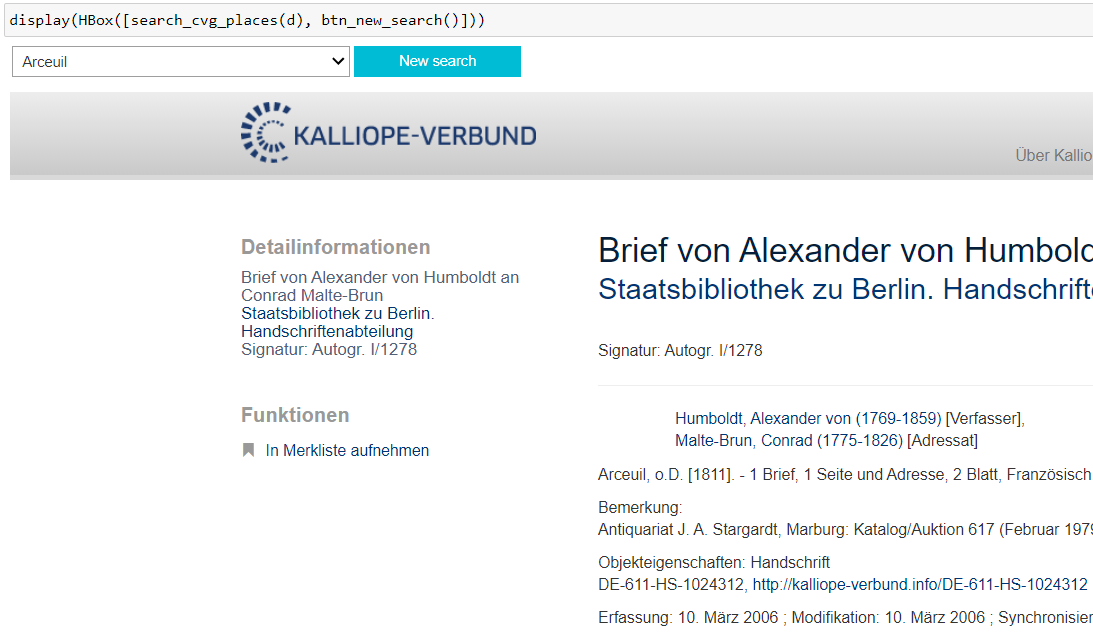
\includegraphics[height=0.5\linewidth]{img/recherche_website.png}
        \caption{Affichage de la page du Kalliope-Verbundkatalog dans l'output.}
    \end{subfigure}
    \begin{subfigure}[b]{0.34\textwidth}
        \centering
        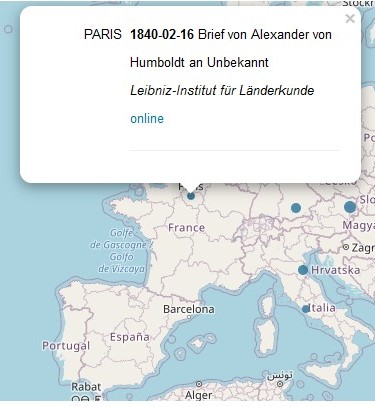
\includegraphics[height=0.9\linewidth]{img/mapviz_1840_radius_popup.jpg}
        \caption{Fenêtre PopUp d'une lettre envoyée à Paris en 1840.}
    \end{subfigure}
    \vspace{-10pt}
\end{figure}
\end{changemargin}
\vspace{-20pt}
D'autre part, l'utilisateur a également accès aux informations des lettres grâce à l'interactivité des cartes. Comme évoqué précédemment, ces dernières sont cliquables et la sélection d'un point par l'utilisateur permet d'afficher une fenêtre PopUp. Ainsi, s'y affiche le lieu d'envoi de la lettre et sa date d'envoi, le nom de l'expéditeur ainsi que du destinataire, le lieu de conservation accompagné du lien vers le catalogue en ligne. 

\begin{wrapfigure}{l}{0.40\textwidth}
\label{wrapfig:carteBerlinInfo}
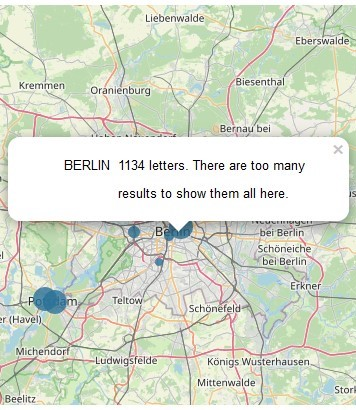
\includegraphics[width=0.40\textwidth]{img/mapviz_toutes_berlin_extrait.jpg}
\caption{Exemple d'affichage : les 1134 lettres de Berlin}
\vspace{-10pt}
\end{wrapfigure}
L'utilisation des Jupyter Notebook apporte ici des contraintes dans la présentation de ces informations. En effet, les cartes sont affichées en format panoramique, c'est-à-dire qu'elles sont moins hautes que longues. Ce format d'affichage n'est pas optimal afin de présenter toutes les informations pour chacune des villes. Seuls les éléments de trois lettres peuvent être affichés sans contrainte. L'utilisateur est invité à se tourner vers le DataFrame pour avoir un accès sans limite aux informations contenues dans la base de données. Toutefois, les DataFrame ne permettent pas à l'utilisateur d'avoir accès au catalogue en ligne de manière aisée puisque les liens qui s'y affichent n'y sont pas cliquables. 

Les données disponibles ne sont pas seulement les données externes récupérées via des \gls{api}. En effet, les données extraites de l'aide à la recherche ont été introduites dans les fonctions de recherche et l'utilisateur peut également y avoir accès. Toutefois, seule une recherche par institutions conservatrices permet d'accéder aux données de la \gls{bbaw} puisqu'il s'agit de la seule information disponible au sein du document Excel : aucune information sur le contenu des lettres conservées par les institutions n'y est informé. Par conséquent, l'utilisateur sélectionne l'institution et dans la cellule de sortie apparaissent deux types de résultats :
\begin{itemize}
    \item les données de l'aide à la recherche présentées sous forme de string\footnote{Une string en Python est une chaîne de caractères.}. Ici sont présents les tiroirs où se trouvent les lettres correspondantes au sein des archives mais aussi le nombre de lettres inventoriées
    \item les données des catalogues en ligne.
\end{itemize}
Les données des catalogues en ligne sont présentées sous deux formes afin de permettre à l'utilisateur de comparer les deux collections. En effet, la collection de la \gls{bbaw} peut être obsolète et non à jour. 

\begin{wrapfigure}{l}{0.61\textwidth}
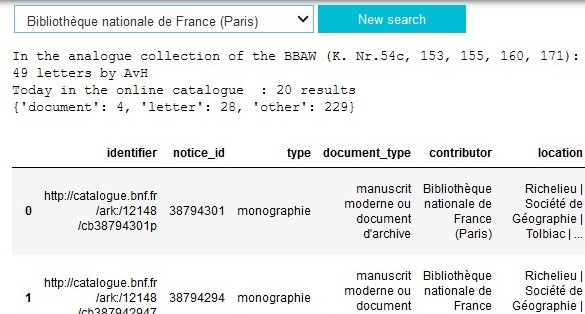
\includegraphics[width=0.61\textwidth]{img/suchemitFindbuchBnF.jpg}
\caption{Exemple : les résultats pour la BnF}
\end{wrapfigure}
Cet exemple ci-contre présente les résultats pour la Bibliothèque nationale de France. Les premières lignes correspondent aux données de l'aide à la recherche montrant que 49 photocopies de lettres provenant de la \gls{bnf} sont stockées dans les archives de la \gls{bbaw}. Ces lignes sont suivies du nombre d'entrées dans notre base de données pour la Bibliothèque nationale de France puis le détail de ces entrées. En effet, une entrée ne représente pas forcément une lettre mais un dossier, un ensemble de documents ou bien une ou plusieurs lettres. Ainsi, le nombre d'entrée pour la Bibliothèque nationale de France est de vingt mais ces vingt résultats représentent finalement 28 lettres et 233 autres documents. Ici, on comprend bien que la collection de la \gls{bbaw} n'est pas à jour et ces lignes permettent de comparer l'état actuel des collections. 

Toutes ces données sont accessibles gratuitement dès lors que l'utilisateur a installé le projet sur son ordinateur. Le projet est open source et est disponible sur un dépôt gitHub.

\section{Accès au projet}
\subsection{Livrable: un dépot github}
La donnée se doit d’être suffisamment contextualisée pour que l’utilisateur puisse en comprendre le sens. Par exemple, le chiffre « 19 » peut représenter une température, un nombre de clients ou un montant. Dès lors, il faut que des informations complémentaires accompagnent les données pour permettre leur contextualisation. Le format du Jupyter Notebook autorise la rédaction d'une documentation riche et explicite accompagnant les cellules de code. Plus le projet sera fourni en documentation et en contextualisation, plus ce dernier sera facilement pris en main par les utilisateurs et sera compris. 

Le dépôt GitHub fait donc office de portail permettant à l'utilisateur d'accéder au projet facilement. Il est accompagné d'un document README, document Markdown, contenant le contexte de développement du projet et quelques lignes de contextualisation historique. Ces informations sont suivies des commandes d'installation pour une installation sur une machine Linux. L'utilisateur doit copier les commandes directement dans son terminal et suivre les instructions afin de lancer le projet et de découvrir la riche correspondance épistolaire d'Alexander von Humboldt directement sur sa propre machine. 

Néanmoins, installer le projet sur sa machine reste une opération technique. Cela entend que l'utilisateur sache utiliser un terminal et comprenne le fonctionnement d'un Jupyter Notebook. Une utilisation via le terminal est loin d'être une opération que le grand public sera capable d'effectuer de manière aisée et sans connaissance préalable. Il serait bien plus confortable pour tous si ces fonctions de recherche et ces visualisations seraient disponibles sur une application web, accessible via les moteurs de recherche. À ce stade du projet, l'accessibilité reste par conséquent limitée à des techniciens à l'aise avec les technologies GitHub et Jupyter Notebook.

\subsection{Communiquer autour du projet}
Communiquer autour du projet c'est apporter de la visibilité, de la compréhension et du contexte supplémentaires aux utilisateurs potentiels. Cette action de communication fait également partie de l'accessibilité du projet puisqu'elle le rend beaucoup plus accessible, beaucoup plus visible auprès des chercheurs à défaut du grand public.

Au cours de mon stage, j'ai eu la chance de présenter mon projet lors de deux conférences. Ces deux conférences ont été des étapes importantes mais aussi de réels défis : prendre la parole en allemand devant du public intéressé, recevoir des retours et des avis sur ce que j'avais réalisé, répondre aux questions afin de lever des incompréhensions ou bien afin d'approfondir des points. 

La première conférence à laquelle j'ai participé a eu lieu au cours d'un événement du \href{https://vdhd2021.hypotheses.org/}{vDHd21}. Le vDHd21 est un événement communautaire de humanistes numériques qui proposent de nombreuses conférences, des publications et des rencontres tout au long de l'année.  Le vDHd est axé sur les expérimentations et les formats alternatifs. Il conçoit une forme d'échanges décentralisée et virtuelle. En plus d'apporter de la visibilité au projet, cela permet à ce dernier de s'ancrer dans la communauté scientifique. 
La seconde conférence fait partie du colloque organisé par la \gls{bbaw} elle-même. Ce colloque se concentre sur les humanités numériques dans le but d'intensifier le dialogue interdisciplinaire dans le domaine. En tant que principale institution de recherche non universitaire de Berlin, ce colloque inscrit la \gls{bbaw} dans cette communauté des \textit{Digital Humanities}. L'événement se concentre sur des sujets pratiques et des exemples d'applications mais aussi sur une réflexion critique de la recherche en humanités numériques. Ainsi, tous les premiers vendredis du mois, une conférence est proposée et se déroule depuis mars 2020 exclusivement de manière virtuelle\footnote{Voir le prgramme sur le site de la \href{https://www.bbaw.de/bbaw-digital/dh-kolloquium}{BBAW}.}. La participation n'est pas exclusivement réservée aux membres de la \gls{bbaw} et à ses partenaires, toutes personnes peut présenter son sujet et proposer une conférence.

Lors de ces deux participations, j'ai été accompagnée par Dr. Gordon Fischer et Christian Thomas. L'idée était de présenter l'extraction des données de l'édition numérique ainsi que leur visualisation cartographique. L'outil \textit{Humboldt Chronotopographie}\footnote{Voir \autoref{sect:chronotopographie}.} a ainsi été exposé pour la première fois depuis son développement au public. En tant que projet expérimental et dont le développement est particulièrement récent, il est important de lui apporter une certaine visibilité afin qu'il puisse prendre de l'ampleur. De plus, il a pour vocation à être collaboratif. Au cours de la conférence, j'ai eu le plaisir de présenter mon projet et particulièrement les visualisations de données réalisées puisqu'elles s'adaptaient particulièrement au sujet de la conférence. Pour ces deux présentations, environ une trentaine d'auditeurs ont répondu à l'appel. 

Cela a été, pour ma part, une occasion de présenter mes réalisations, d'expliquer ce qui a été produit mais aussi de le diffuser. De cette manière, les participants ont eu accès au GitHub où est disponible tout le projet et savent le chemin à emprunter afin d'avoir accès aux données de la correspondance.

\part{Enrichir des projets numériques de la BBAW grâce aux données externes}

\chapter{correspSearch : collaborer autour des échanges épistolaires}
\chaptermark{correspSearch}
\label{chap:cSBesoins}
Le portail web correspSearch est développé depuis avril 2014 par \gls{telota} de la \gls{bbaw} et en coopération avec le \gls{tei} Correspondence \gls{sig} ainsi que d'autres chercheurs participants. En tant qu'initiative de la \gls{bbaw}, ce projet est financé par des tiers. 
Le modèle de données en réseau de l'\textit{edition humboldt digital}\footnote{Voir le modèle de données détaillé, \autoref{fig:donneesReseau}} permet de rendre compte du lien entre l'édition et correspSearch : l'édition numérique met à disposition les métadonnées de la correspondance d'Alexander von Humboldt et, en contrepartie, elle appelle les métadonnées des lettres éditées par d'autres éditions afin d'enrichir son propre corpus. Toutes ces données échangées sont structurées en \gls{cmif}. Le \gls{cmif} ainsi que le projet correspSearch sont les sujets de ce chapitre. 


\section{correspSearch : le projet et ses objectifs}
CorrespSearch est un projet initié par la \gls{bbaw} et dirigé par \href{https://www.bbaw.de/die-akademie/mitarbeiterinnen-mitarbeiter/dumont-stefan}{Stefan Dumont}, chercheur et ingénieur d'étude au sein de \gls{telota}, le pôle des humanités numériques de la \gls{bbaw}. Le but du projet correspSearch est de mettre à disposition des chercheurs et du grand public un répertoire de diverses éditions de lettres sur une interface web.

Le projet est parti d'un constat : les lettres comptent parmi les sources importantes de la recherche historique. Elles abordent et commentent tous les sujets possibles qui ont intéressés leur rédacteur. Témoins de leur époque, elles permettent également d'étudier les réseaux épistolaires entre diverses personnes. Néanmoins, pour des raisons éditoriales, la correspondance historique n'est éditée que par extraits. En effet, seul l'échange de lettres entre deux personnes est éditée ou bien toute la correspondance d'une seule et même personne. Il est alors difficile d'explorer un large corpus épistolaire sans effectuer des recherches de longue haleine sur plusieurs éditions de lettres. Le service correspSearch a pour but de pallier à ces problèmes en effectuant le premier pas vers une mise à disposition de toutes les lettres éditées sur un même service et en redirigeant le chercheur vers les publications originales.

\begin{wrapfigure}{r}{0.7\textwidth}
\centering
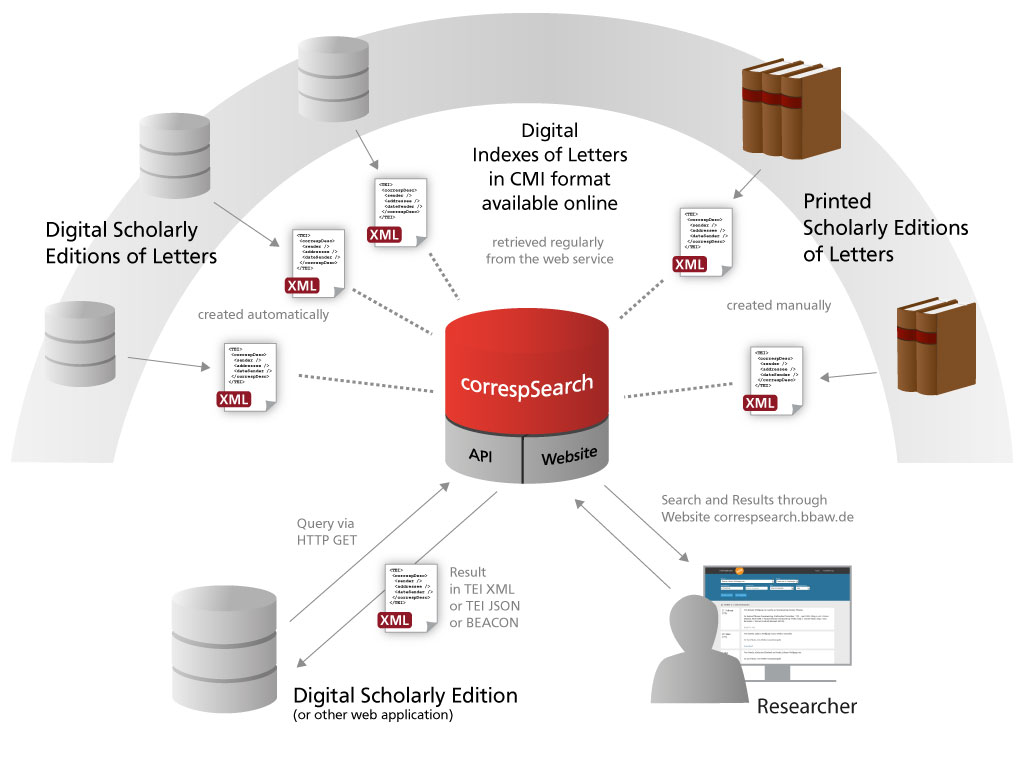
\includegraphics[width=0.7\textwidth]{img/correspSearchfonctionnement.png}
\caption{Fonctionnement de correspSearch.}
\vspace{-10pt}
\end{wrapfigure}

Les métadonnées des lettres provenant de diverses éditions imprimées et numériques ainsi que d'index numériques sont centralisées et distribuées sur le site ouvertement sous une licence CC-BY 4.0, licence libre. Le service web agrège les métadonnées de correspondance de ces index numériques qui sont hébergés ailleurs sur le web, crées et fournis par divers projets d'éditions savantes. Les métadonnées, sous format \gls{xml}-\gls{tei}, fournies par ces index de correspondances sont ensuite récupérées par correspSearch à intervalles réguliers dans l'année permettant une actualisation fréquente. L'utilisateur peut effectuer une recherche dans le répertoire de correspSearch et avoir accès en une seule recherche à toutes ces éditions. Grâce à la recherche avancée, le service web propose d'effectuer des recherches par nom d'expéditeur, nom de destinaire, lieu et date de rédaction de la lettre. 

La base de données correspSearch représente une collection constamment enrichie : les éditions savantes de lettres numériques sont de plus en plus nombreuses. Le service web ne fixe pas de limites concernant la période historique ou bien le lieu de production de la correspondance. Toute édition intéressée a la possibilité de déposer ses données en \gls{cmif} par le biais du service web. Il existe déjà une variété d'organisations numériques mettant à disposition des données issues de correspondances épistolaires. Le service correspSearch est conçu pour s'intégrer dans ce paysage déjà varié et cherche à le compléter. Pour les ressources purement archivistiques, il existe déjà divers formats et services numériques comme le format \gls{ead} et le catalogue du Kalliope-Verbund\footnote{Voir \autoref{sub:kalliope}}. C'est pour cela que correspSearch met à disposition non pas des données archivistiques mais des données issues d'édition numérique ou bien imprimée, c'est-à-dire la correspondance ayant fait l'objet d'édition scientifique accompagnée de commentaires critiques.

CorrespSearch est un projet qui sans la collaboration des éditions et des chercheurs ne fonctionnerait pas ou moins bien. C'est l'une des raisons pourquoi le site invite à la collaboration\footnote{Voir l'onglet \textbf{participate} sur le site de correspSearch : \href{https://correspsearch.net/en/participate.html}{correspsearch.net/en/participate.html}} et propose de nombreux outils afin d'aider à convertir les données de chacun en \gls{cmif}. Fournir un fichier \gls{cmif} présente de nombreux avantages pour les projets de recherche qui participent à l'enrichissement de correspSearch. En effet, cela leur permet de rendre leurs lettres éditées plus accessibles à la communauté des chercheurs mais également de lier leur édition avec d'autres éditions. D'autre part, ces projets contribuent à faciliter la recherche puisque les correspondances sont centralisées dans un seul et même service. 

Le chercheur, qu'il participe au sein de correspSearch ou bien qu'il soit un simple utilisateur du service web, a la possibilité d'accéder aux données via l'\gls{api} mise à disposition. Cette \gls{api} fonctionne par des requêtes \gls{http} GET et renvoie un résultat sous divers formats\footnote{Voir l'onglet \href{https://correspsearch.net/en/api.html}{API de correspSearch}.} dont le \gls{cmif}.

\section{Le format CMI (CMIF)}
Afin que correspSearch puisse agréger les métadonnés de lettres provenant de divers sources, les métadonnées doivent être fournies dans un format normalisée et lisible par machine. Le format \gls{xml}-\gls{tei} semble approprié dans ce contexte car il est utilisé dans les éditions numériques depuis plusieurs années déjà et est devenu une norme. De plus, il est possible de s'appuyer sur les travaux du Correspondance \gls{sig} qui a développé l'élément \texttt{correspDesc} pour les \gls{tei} \textit{guidelines}. Cette extension de la \gls{tei} fournit un jeu de balises pour enregistrer des métadonnées spécifiques à la correspondance dans le \texttt{teiHeader}, telles que l'expéditeur, le destinataire et le lieu d'écriture. Après avoir subi quelques modifications \texttt{correspDesc} a éte intégré dans les \textit{guidelines} de la \gls{tei} en avril 2015\footnote{\cite{dumont_correspsearch_2016}}.

Le \gls{tei} Correspondance \gls{sig} a également développé le \gls{cmif} et rend possible une standardisation des métadonnées de lettres. L'essence du document \gls{cmif} consiste en de multiples éléments \texttt{correspDesc}, chacun correspondant à une lettre. Cependant les éléments \texttt{correspDesc} sont utilisés de manière très restreinte afin de permettre un traitement automatique par la suite. Par exemple, la balise \texttt{correspAction} n'accepte que deux éléments dans son attribut \texttt{@type} qui sont \texttt{sent} et \texttt{received}. Cette balise accepte seulement les balises \texttt{persName}, \texttt{placeName} et \texttt{date} en tant que balises enfants. L'emploi très restreinte de balises est nécessaire afin de permettre une interopérabilité sans aucune intervention humaine. Cette restriction impose également l'encodage d'informations limitées aux métadonnées de bases concernant les lettres, à savoir : l'expéditeur, le destinaire, le ou les lieux de réception et les dates. L'édition de laquelle la lettre est issue est encodée dans l'attribut \texttt{@source} de la balise \texttt{correspDesc} sous forme d'identifiant.

La spécification \gls{cmif} recommande fortement un alignement à des référentiels grâce à l'emploi d'identifiants provenant de notice d'autorité afin de distinguer les personnes et les lieux. Pour chaque entité, il existe une notice avec un identifiant unique, indépendant du projet et permanent. Cet identifiant qui peut être référencé par tous est largement utilisé sur le web comme référence\footnote{À ce propos, je renvoie le lecteur vers la \autoref{part:donnéesExternes}}. Dans le contexte de correspSearch, l'utilisation de fichiers d'autorités permet d'éviter l'utilisation de chaînes de caractères encodées par des humains et dont les erreurs, variantes orthographiques et homonymes sont fréquents. Ainsi, l'outil de recherche de l'interface correspSearch effectue une recherche sur les identifiants des notices d'autorité encodés au sein des fichiers \gls{cmif}. CorrespSearch acceptent diverses notices d'autorité pour les personnes : l'identifiant \gls{gnd} mis en place par la Bibliothèque nationale allemande, l'identifiant de la \gls{bnf}, le \gls{ndl}, notice d'autorité japonaise ainsi que l'identifiant \gls{viaf}. Pour les lieux, ce sont les identifiants GeoName qui sont pris en charge. Dans le contexte des technologies du web sémantique, l'utilisation d'identifiants uniques et normalisés pour les entités communes est cruciale afin d'assurer le partage des données de recherche en tant que données ouvertes et liées. 

Maintenant que les diverses balises employées au sein d'un fichier CMIF et que les notices d'autorité acceptées ont été présentées, voici ce à quoi ressemble l'encodage d'une lettre en format CMI\footnote{Cet exemple est celui présenté \href{https://correspsearch.net/de/dokumentation.html}{sur le site correspSearch} au sein de la documentation pour le format CMI.} :
\begin{figure}[h!]
    \centering
         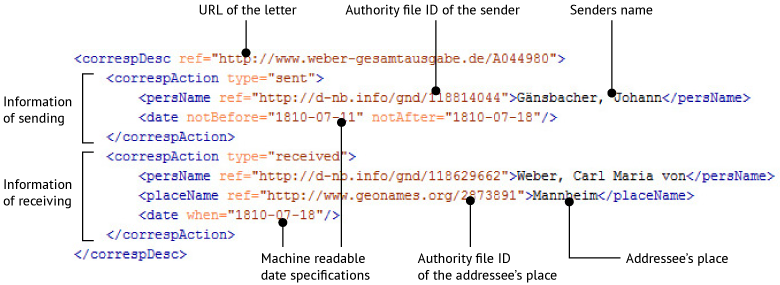
\includegraphics[scale=0.5]{img/cmif_letter.png}
         \caption{Exemple d'une lettre en CMIF.}
         \label{fig:lettreCMIF}
\end{figure}

Depuis peu, la possibilité de faire référence au document archivistique d'une lettre a été implémentée. Cette référence sous forme d'\gls{uri} est stockée au sein de \texttt{correspDesc/@corresp}. C'est exactement dans ce contexte que le \textit{cS matching tool} s'est développé.


\chapter{De la conception au développpement}
\section{Les objectifs du \textit{cS matching tool}}
\label{sect:objectifcSMT}
Jusqu'alors il était possible de faire référence à l'édition d'une lettre, qu'elle soit imprimée ou numérique, au sein du \texttt{correspDesc/@ref} dans un document \gls{cmif}. La référence vers le document manuscrit conservé dans un centre d'archives s'insère dans l'attribut \texttt{@corresp} de cette même balise. Cette possibilité de référence a été implémentée il y a peu. Les lettres déjà versées dans correspSearch avant l'implémentation de cette fonctionnalité ne sont donc pas pourvues de cette référence. L'idée, initiée par Stefan Dumont, chercheur et ingénieur de recherche au sein du pôle \gls{telota} de la \gls{bbaw}, est donc de créer un outil permettant d'insérer les liens vers la référence archivistique, c'est-à-dire au sein de \texttt{correspDesc/@corresp} pour chacune des lettres correspondantes. 

Les données utiles à ce projet sont celles déjà versées sur correspSearch ainsi que celles du Kalliope-Verbundkatalog où les références aux lettres de la correspondance von Humboldt sont les plus importantes. Le but est donc de pouvoir faire correspondre une lettre des données du Kalliope-Verbunkatalog à celles de correspSearch. Si les données sont les mêmes au sein des deux sets de données alors il s'agit de la même lettre. Par conséquent, le lien vers le Kalliope-Verbundkatalog peut être ajouté à la balise correspondante au sein des données de correspSearch. Afin d'identifier une lettre, quatre éléments sont nécessaires :
\begin{itemize}
    \item l'expéditeur
    \item le destinataire
    \item la date d'envoi
    \item le lieu d'envoi
\end{itemize}

Néanmoins, ces informations ne sont pas toujours complètes. Beaucoup de lettres ne possèdent pas d'information concernant la date d'envoi ou le lieu d'envoi. C'est particulièrement fréquent quand deux correspondants s'échangent très régulièrement des lettres et vivent dans la même ville. Bien souvent les partenaires de correspondance d'Alexander von Humboldt sont plus méticuleux dans la rédaction de ces informations. La date ainsi que le lieu d'envoi sont d'une manière générale plus complets. Humboldt, quant à lui, ne prend pas souvent la peine d'indiquer la date exacte sur ses lettres quand il vivait à Berlin et se suffisait d'un simple "ce matin" ou bien "hier". Difficile ensuite d'identifier pleinement cette lettre et par conséquent, il existe deux matches possibles : 
\begin{itemize}
    \item ceux qu'on appelle les \textit{full matches} c'est-à-dire les lettres pour lesquelles les quatre éléments cités ci-dessus correspondent
    \item les \textit{possible matches} pour lesquels l'expéditeur, le destinataire ainsi que la date d'envoi correspondent mais pas le lieu.
\end{itemize}
On peut se demander si l'expéditeur, le destinataire ainsi que la date d'envoi ne sont pas suffisants pour considérer un match comme complet. Il est possible qu'Humboldt ait envoyé une lettre le même jour à la même personne. Cela arrive et c'est pour cela que l'utilisateur à la possibilité ensuite de confirmer ou non ces matches considérés comme possibles. Aussi, les données issues de correspSearch sont bien souvent plus complètes que celles du Kalliope-Verbundkatalog. En effet, les données de correspSearch proviennent des éditions imprimées et/ou numériques des correspondances, c'est-à-dire que des chercheurs ont ajouté des commentaires critiques et ont ajouté des informations à propos de ces lettres. Ils ont identifié, pour certaines lettres, des lieux d'envoi qui n'apparaissent pas explicitement dans les documents d'archives. C'est pour cela qu'il est important de laisser l'utilisateur décider s'il s'agit d'un match ou non. Ces matches sélectionnés par l'utilisateur sont ensuite ajoutés au fichier \gls{cmif} et seront téléchargeables. 

Par conséquent, l'outil doit intégrer diverses fonctionnalités :
\begin{itemize}
    \item prendre en charge des fichiers \gls{cmif}
    \item présenter les possibles matches afin que l'utilisateur puisse les sélectionner ou non
    \item ajouter l'\gls{uri} correspondante au sein de \texttt{correspDesc/@corresp}
    \item les matches, une fois intégrés au document correspondant, doivent être téléchargeables en \gls{cmif} directement sur l'ordinateur de l'utilisateur
\end{itemize}

Il serait également utile que l'utilisateur puisse décider s'il souhaite télécharger le fichier contenant toutes les lettres de correspSearch avec les \gls{uri} ajoutées aux balises correspondantes ou bien s'il télécharge un fichier \gls{cmif} contenant uniquement les matches et au sein duquel les lettres qui n'ont trouvé aucune corrélation auront été supprimées.

Cet outil est destiné aux techniciens de correspSearch afin d'enrichir leurs données avec l'ajout d'une référence supplémentaire. La cible n'est pas le grand public. Toutefois, l'expérience utilisateur doit être suffisamment intuitive afin que le technicien ou bien la personne qui s'occupera d'effectuer cette tâche puisse la réaliser de manière aisée sans avoir à lire une documentation complète sur la manière dont fonctionne cette application. Étant donné que de nombreuses personnes effectuant leur stage au sein du projet \textit{Alexander von Humboldt auf der Reise} sont plutôt familières à la recherche qu'à l'ingénierie et qu'il s'agit d'une tâche qui pourrait être réalisée par ces dernières, il est important qu'une interface utilisateur soit développée. C'est pour cela qu'il a été décidé de créer une application web qui pourrait être installée localement sur l'ordinateur prêté aux stagiaires. Le développement de l'outil est donc mixte : un développement \textit{back end} contenant toute la logique de l'application et un développement \textit{front end} pour l'interface utilisateur.

\section{Développements back end et front end}
On dissocie le développement \textit{back end} du développement \textit{front end}. Le \textit{back end} fait référence à la partie du code qui est invisible de l'utilisateur contrairement au \textit{front end} qui représente la partie visible, l'interface utilisateur c'est-à-dire ce qui est affiché dans le navigateur de l'utilisateur. Au sein de ce projet, la partie \textit{back end} est développée en Python tandis que le \textit{front end} en \gls{html} et \gls{css}. L'application en elle-même a été développée avec le \textit{framework} Flask. 
\subsection{Back end : algorithmie}

\subsubsection{Le choix du langage de programmation et du framework}
Puisque l'application a vocation à être développée de manière \textit{standalone}, j'ai été particulièrement libre de choisir le langage dans lequel je souhaitais la programmer. Le choix du langage de programmation s'est arrêté sur Python pour plusieurs raisons. La première était le fait de rester dans une certaine continuité avec la mission que j'avais effectuée précédemment à savoir le développement de fonctionnalités de recherche et de visualisations de données. Ces dernières, développées dans des Jupyter Notebooks, ont été entièrement rédigées en Python\footnote{Voir \autoref{chap:rechercheEtViz}.}. Par ailleurs, il y a la question de la maintenance de l'application. Afin que cette application puisse être utilisée de manière durable, elle doit être maintenue. La personne qui sera désignée pour cette tâche doit connaître le langage dans lequel l'application est programmée. Python est un langage largement connu. Il est également apprécié par de nombreux pédagogues qui considèrent Python comme un langage où la syntaxe permet une initiation aisée aux concepts de base de la programmation\footnote{\cite[préface]{elkner_how_nodate}.}. 

Un \textit{framework}, aussi appelé environnement de développement en français, désigne un ensemble de composants logiciels structurels. Il sert à créer les grandes lignes ou les fondations d'un logiciel. Il guide ainsi l'architecture logicielle et conduit parfois le développeur à respecter des patrons de conception de part les bibliothèques dont il est constitué. Toutes ces technologies m'étaient connues avant le début de la mission et cela me permettait de me concentrer sur la logique de l'application et non l'apprentissage d'un nouveau langage ou d'un nouveau \textit{framework}. Flask est un \textit{framework open-source} pour le langage Python. Ce \textit{framework}, déjà connu puisqu'il est enseigné à l'École nationale des chartes, permet le développement d'application web. Sa documentation est particulièrement détaillée et contient de nombreux morceaux de code facilement adaptables à nos projets\footnote{La documentation est disponible sur \href{https://flask.palletsprojects.com/en/2.0.x/}{flask.palletsprojects.com}}. À ce sujet, Gilles Babinet\footnote{\cite{babinet_12_2020}} informe qu'on dit souvent que les programmeurs actuels ne programment plus mais que leur métier consiste à coller des morceaux de programmes les uns avec les autres. Les développements sont sophistiqués et reposent sur des ensembles de codes écrits par d'autres. Il faut toutefois noter que cette dynamique s'insère dans la communauté de l'\textit{open source}. Les programmeurs utilisent des portions de code disponibles en \textit{open source} qu'ils retournent à la communauté en mettant à disposition leur code sur des plateformes comme GitHub. Les licences \textit{open source} ont le point commun de mettre l'accent sur la liberté de l'individu d'aller modifier le code source et de se l'approprier pour ensuite, pouvoir créer de la valeur ajoutée qui retourne à l'ensemble de la communauté.

\subsubsection{La structure de l'application}
\begin{wrapfigure}{r}{0.45\textwidth}
\centering
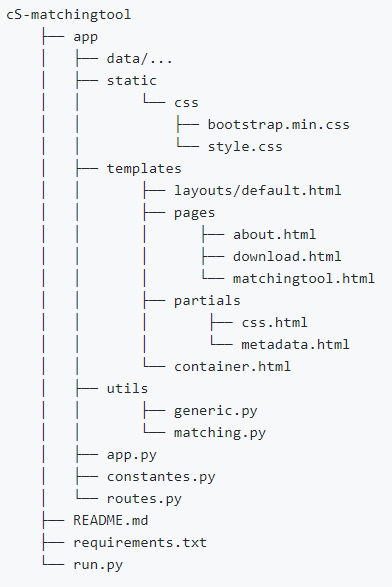
\includegraphics[width=0.45\textwidth]{img/structure_csMatchingTool.png}
\caption{La structure de l'application}
\vspace{-15pt}
\end{wrapfigure}
La structure du projet est relativement simple : l'application est contenue dans le dossier \texttt{app/}. En son sein, se trouve un dossier prêt à recevoir les données puis deux autres dossiers destinés au \textit{front end} (\texttt{static/} pour les styles et \texttt{templates/} pour les fichiers \gls{html}). Les fonctions logiques sont stockées dans deux fichiers \texttt{.py} différents : les fonctions génériques contenues dans \texttt{generic.py} puis la fonction qui permet de corréler les données est stockée dans \texttt{matching.py}. Les routes sont les fonctions qui font le lien entre le \textit{front end} et le \textit{back end}, c'est-à-dire qu'elles vont chercher dans le \textit{back end} les données afin de les mettre à disposition de l'utilisateur dans le \textit{front end}. Ces fonctions sont enregistrées dans le fichier \texttt{routes.py}. Toute la configuration de l'application est répartie dans \texttt{app.py} et \texttt{constantes.py}.

Quand l'utilisateur installe l'application sur son serveur local, aucune donnée n'est encore stockée en son sein. Seul un dossier est disponible et est prêt à recevoir les données qui devront être comparées. Puisque ces données vont se limiter à deux fichiers à savoir : un fichier pour les données du Kalliope-Verbundkatalog et puis un second pour celles issues de correspSearch, développer toute une base de données avec SQLAlchemy n'a pas semblé nécessaire. 

\subsubsection{La librairie \texttt{xml.etree} pour prendre en charge des fichiers XML}

La librairie \texttt{xml.etree}\footnote{Voir la \href{https://docs.python.org/3/library/xml.etree.elementtree.html}{documentation}.} permet de se déplacer dans l'arbre de fichiers \gls{xml} en le parsant. En effet, \gls{xml} est un format hiérarchique et la meilleure façon de se représenter ce type de fichier est sous la forme d'un arbre. Cette bibliothèque dispose de deux classes qui sont \textit{ElementTree} qui représente l'ensemble du document \gls{xml} sous forme d'un arbre et \textit{Element} qui est la représentation d'un seul noeud au sein de cet arbre. Ainsi, dans notre algorithme, le \texttt{tree} représente toujours notre document. Toutefois, notre fonction compare deux fichiers \gls{xml} différents. Par conséquent, deux arbres sont présents dans notre algorithme, un pour chaque document. 

Afin de récupérer les données voulues au sein de chacun des documents \gls{xml}, certaines fonctions de la librairie \texttt{xml.etree} sont intéressantes :
\begin{itemize}
    \item \texttt{Element.findall()} trouve seulement les éléments enfants de l'élément actuel. Il ne faut pas la confondre avec la fonction \texttt{Element.find()} qui trouve uniquement le premier élément enfant de la balise indiquée en tant qu'argument de cette fonction. 
    \item \texttt{Element.text} permet d'accéder au texte contenu dans la balise.
    \item \texttt{Element.attrib} permet de récupérer les attributs d'un élément.
    \item \texttt{Element.iter()} permet d'itérer de manières récursive sur les balises qui lui sont inférieures c'est-à-dire les éléments enfants mais également les éléments de ses enfants. 
\end{itemize}

\subsubsection{Logique algorithmique}
 \begin{figure}[h!]
    \centering
         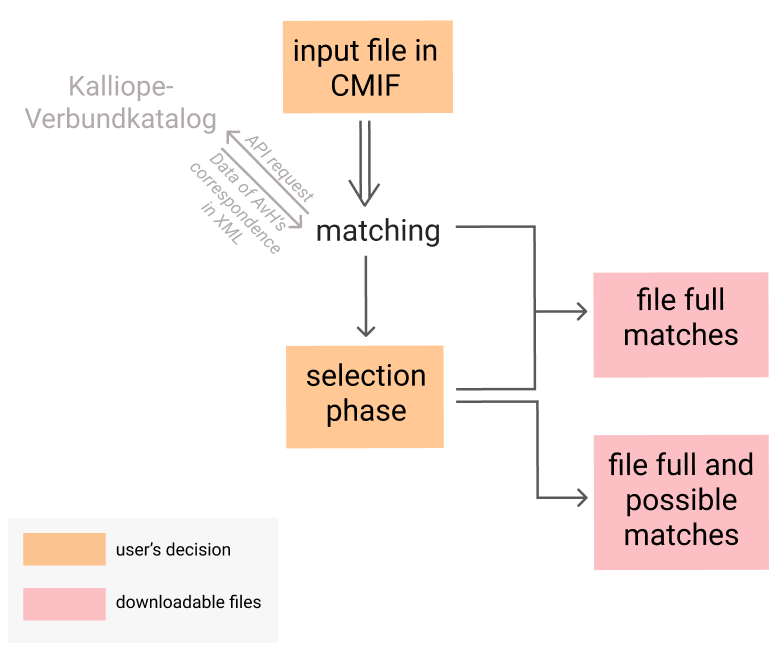
\includegraphics[scale=0.6]{img/schema_matching.png}
         \caption{Logique algorithmique de l'application schématisé}
         \label{fig:schemaMatching}
\end{figure}

 Afin que l'algorithme se lance, la première étape est le dépôt d'un fichier \gls{cmif} par l'utilisateur contenant des lettres de la correspondance d'Alexander von Humboldt. Tout comme les données du Kalliope-Verbundkatalog qui seront requêtées sur l'\gls{api} correspondante, le document de l'utilisateur est enregistré dans le dossier \texttt{data/} prévu à cet effet. Les données sont stockées dans leur format d'origine à savoir en \gls{xml}-\gls{tei} et plus particulièrement en \gls{cmif} pour celles de l'utilisateur. Une condition a été implémentée afin de vérifier que le document déposé par l'utilisateur est un document \texttt{.xml}, si cela n'est pas le cas un message d'erreur est alors envoyé à l'utilisateur. Une fois que le fichier valide est déposé alors la fonction \texttt{matching()}\footnote{Voir la fonction disponible sur le \href{https://github.com/edition-humboldt-collection/cS-matchingtool/blob/main/app/utils/matching.py}{GitHub du projet}.} permettant de corréler les données est appelée. À chaque nouvelle utilisation, l'application envoie deux requêtes à l'\gls{api} du Kalliope-Verbundkatalog afin de récupérer les lettres reçues ainsi que les lettres envoyées par Alexander von Humboldt. Ces deux requêtes permettent de couvrir l'ensemble de la correspondance de Humboldt. Le format demandé lors de ces deux requêtes est \gls{mods} afin d'obtenir davantage d'informations sur les lettres comme notamment les \gls{uri} vers les fichiers d'autorité des expéditeurs et destinataires de lettres\footnote{Voir l'annexe à ce sujet, présentant deux encodages de lettre, l'un en format MODS et le second en DC, l'annexe \ref{annexe:MODSetDC}.}. 

La fonction \texttt{matching()} se déplace à travers l'arbre du document contenant les données du Kalliope-Verbundkatalog et stocke dans diverses variables les éléments que nous souhaitons faire correspondre avec les données du document \gls{cmif} de l'utilisateur. Pour chacune des lettres du Kalliope-Verbundkatalog, l'identifiant de la lettre qui est l'\gls{uri} vers le site du Kalliope-Verbundkatalog, le lieu d'envoi ainsi que l'\gls{uri} de la notice d'autorité de l'expéditeur et du destinataire sont stockés dans des variables adaptées. Ces données stockées, la fonction passe ensuite au document contenant les données de l'utilisateur. Chaque élément que nous souhaitons corréler sont également stockés dans des variables. Les éléments issus du Kalliope-Verbundkatalog et ceux issus du fichier de l'utilisateur sont ensuite comparés c'est-à-dire l'expéditeur de la lettre du Kalliope-Verbundkatalog avec celui de correspSearch, le destinaire, le lieu d'envoi et la date de rédaction. Quand il s'agit d'un \textit{full match} alors l'\gls{uri} du Kalliope-Verbundkatalog est ajouté au sein du fichier \gls{cmif} dans l'attribut \texttt{@corresp} de la balise \texttt{correspDesc} de la lettre correspondante. Les \textit{possible matches} sont, quant à eux, stockés dans une liste. La fonction renvoie cette liste et leur quantité. Ces matches seront mis à disposition de l'utilisateur qui pourra alors sélectionner ceux qu'il considère comme des lettres correspondantes. Les \gls{uri} vers le Kalliope-Verbundkatalog des lettres sélectionnées par l'utilisateur sont par la suite ajoutées au fichier \gls{cmif}.

Lors de ce processus, l'utilisateur a la possibilité de télécharger à deux étapes différentes le fichier contenant les matches. En effet, il peut télécharger les \textit{full matches} avant que les \textit{possible matches} soient insérés au document. Une fois que l'étape de sélection des \textit{possible matches} à intégrer au document est terminée, l'utilisateur peut télécharger le document complet c'est-à-dire contenant les \textit{full matches} qui ont été ajoutés de manière automatique et ceux sélectionnés par l'utilisateur.

\subsection{Front end : interface utilisateur}
\subsubsection{Les langages de programmation et le framework}
Puisqu'on ne connait pas le niveau technique de la personne qui utilisera cette application, il était important de développer une interface utilisateur. En programmation, cette interface, affichée dans le navigateur web de l'utilisateur est appelée \textit{front end} et est programmée, dans notre projet, en \gls{html} et \gls{css}. Le \gls{html} est un langage de balisage conçu pour les pages web. Ce langage peut maintenir du contenu, créer des formulaires de saisie, inclure toutes sortes de ressources multimédias. Il permet également d'écrire de l'hypertexte et de structurer de manière sémantique la page web. Il est aujourd'hui très utilisé conjointement au \gls{css}. Le \gls{css} est ce qu'on appelle également des feuilles de style en cascade. Il s'agit d'un langage informatique qui décrit la présentation des documents structurés en \gls{html} ou \gls{xml}. 
Dans le projet cS matching tool, ces documents sont stockés dans divers dossiers :
\begin{itemize}
    \item \texttt{static/css/} qui contient tous les styles \gls{css} pour les éléments \gls{html}
    \item \texttt{templates/} contenant les fichiers \gls{html} des modèles de pages
\end{itemize}

Le \textit{framework} Bootstrap a également été largement utilisé afin de programmer le \textit{front end} de l'application web. Bootstrap, gratuit et \textit{open source}, est une collection d'outils pour développer le design de sites et d'applications web. Il contient des codes \gls{html} et \gls{css}, des formulaires, boutons, outils de navigations et éléments interactifs. Il est également livré avec plusieurs composants JavaScript sous la forme de plugins jQuery permettant de fournir des éléments supplémentaires comme des infobulles ou encore des carrousels. Chaque composant Bootstrap se compose d'une structure \gls{html}, de déclarations \gls{css} et, dans certains cas, de code JavaScript associé. Une fois utilisé dans un projet, Bootstrap fournit des définitions de style de base pour tous les éléments \gls{html} et le développeur peut modifier ces styles ou en ajouter comme bon lui semble.  

\subsubsection{Le design de cS matching tool}
Quand on explore les différents sites des projets initiés par la \gls{bbaw}, on remarque plusieurs ressemblances. Le menu est toujours présenté sous la forme d'une barre latérale en haut du site internet et contient le nom du projet en gras positionné à gauche suivit des sous-éléments du menu. La présentation des informations s'affiche sous la forme de trois colonnes, elles-mêmes constituées de cases pour chaque nouvelle information\footnote{Voir l'annexe \ref{annexe:designBBAW}.}. Les couleurs utilisées sont régulièrement les mêmes.

\begin{wrapfigure}{r}{0.6\textwidth}
\centering
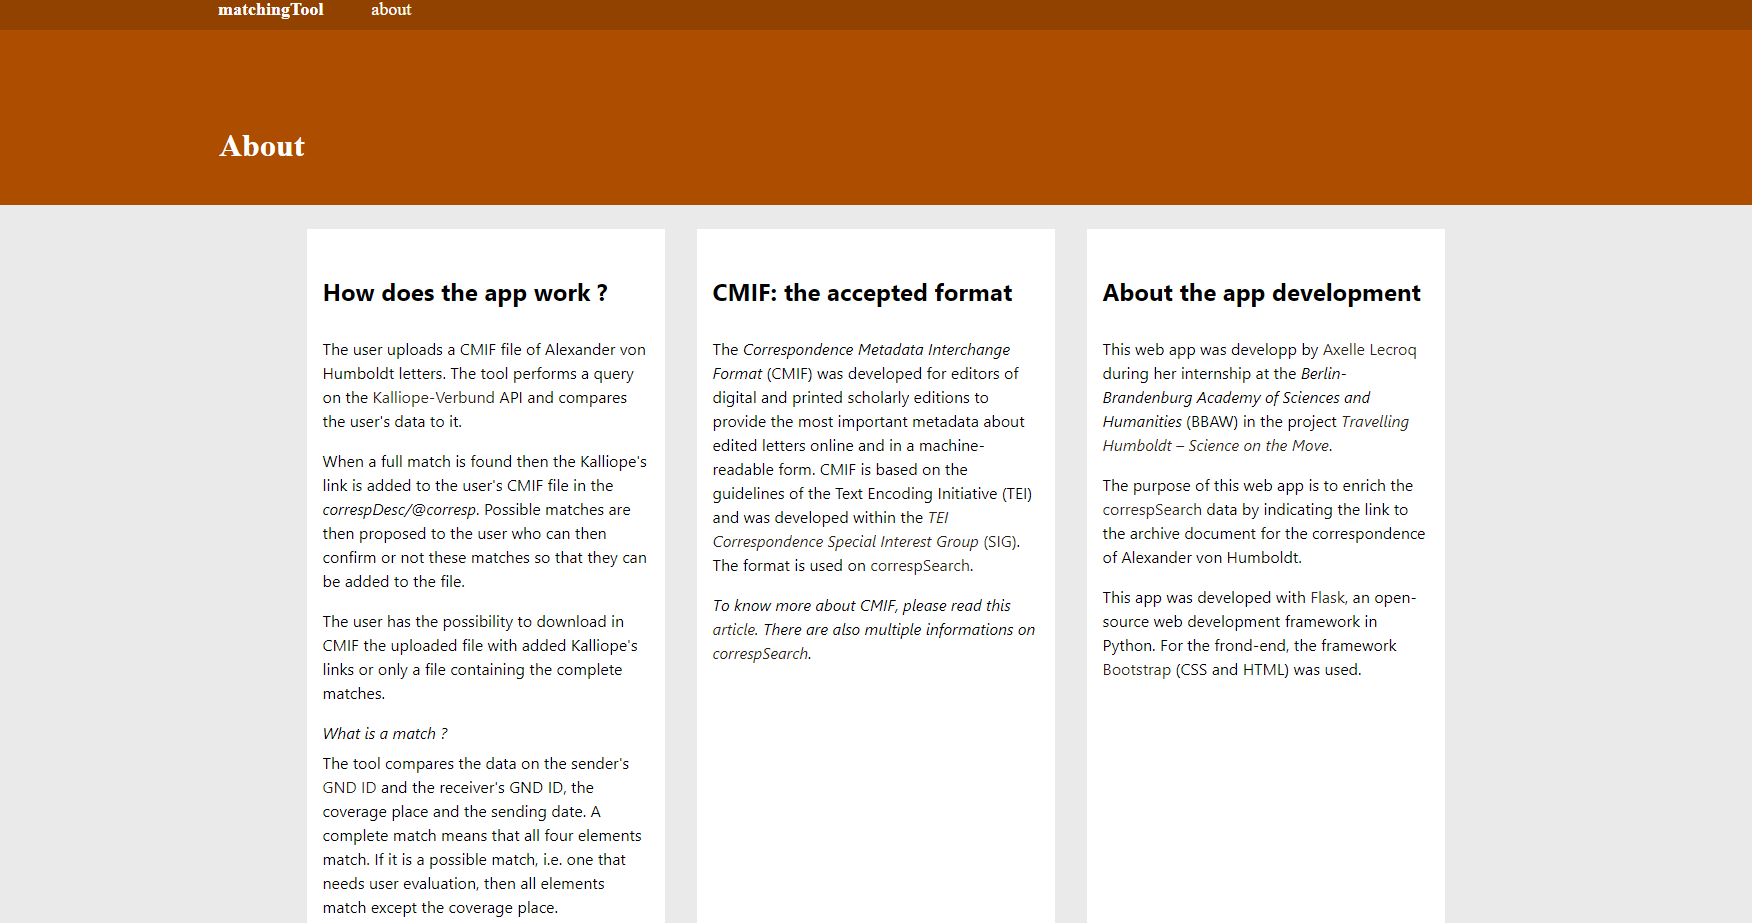
\includegraphics[width=0.6\textwidth]{img/csMT_about.png}
\caption{Page \texttt{about} du cS matching tool}
\vspace{-10pt}
\end{wrapfigure}
Ainsi, au sein du cS matching tool, les couleurs choisies sont semblables à celles utilisées pour le \href{https://edition-humboldt.de/index.xql?l=en}{site} de l'édition numérique des carnets de voyages d'Alexander von Humboldt. En effet, la couleur du fond du cS matching tool est le gris qui est régulièrement employé\footnote{Voir l'annexe \ref{annexe:designBBAW}, (a), (b)} sur les sites de la \gls{bbaw} tout comme l'ocre, particulièrement choisi pour la couleur des boutons ou des éléments sélectionnés dans la barre du menu. La structure de la \gls{bbaw} d'une présentation divisée en trois colonnes a été mise en place pour la page \texttt{about} qui apporte des informations supplémentaires autour du projet à savoir : autour du développement, à propos de la logique algorithmique de l'application et au sujet du format CMI.

\begin{wrapfigure}{r}{0.6\textwidth}
\centering
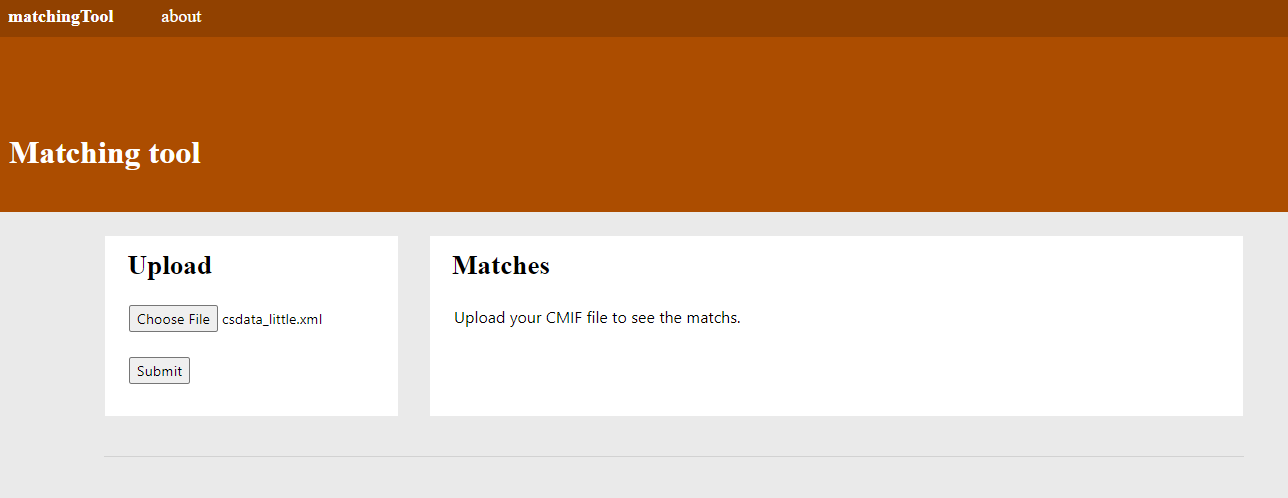
\includegraphics[width=0.6\textwidth]{img/csMT_page1.png}
\caption{Interface permettant à l'utilisateur de glisser son document CMIF}
\vspace{-10pt}
\end{wrapfigure}

Pour ce qui est de la présentation des fonctionnalités, celle-ci a pour vocation d'être la plus simple possible afin de faciliter l'utilisation de l'outil. L'utilisateur voit apparaître deux colonnes : celle de gauche permet de déposer le fichier \gls{cmif} qui a pour but d'être enrichi des liens vers le Kalliope-Verbundkatalog, celle de droite est dans l'attente de présenter les matches possibles. Une fois que le fichier est déposé et que l'utilisateur a cliqué sur le bouton \texttt{submit}, un indicateur de chargement apparaît afin d'indiquer le lancement de l'outil et de ne pas laisser l'utilisateur dans l'attente sans nouvelle information. Sans cet indicateur, il est difficile de savoir si l'outil est lancé ou si l'application rencontre un bug puisque l'application a besoin d'un certain temps avant d'afficher l'étape suivante : la sélection de matches pas l'utilisateur.

\begin{figure}[h!]
    \centering
         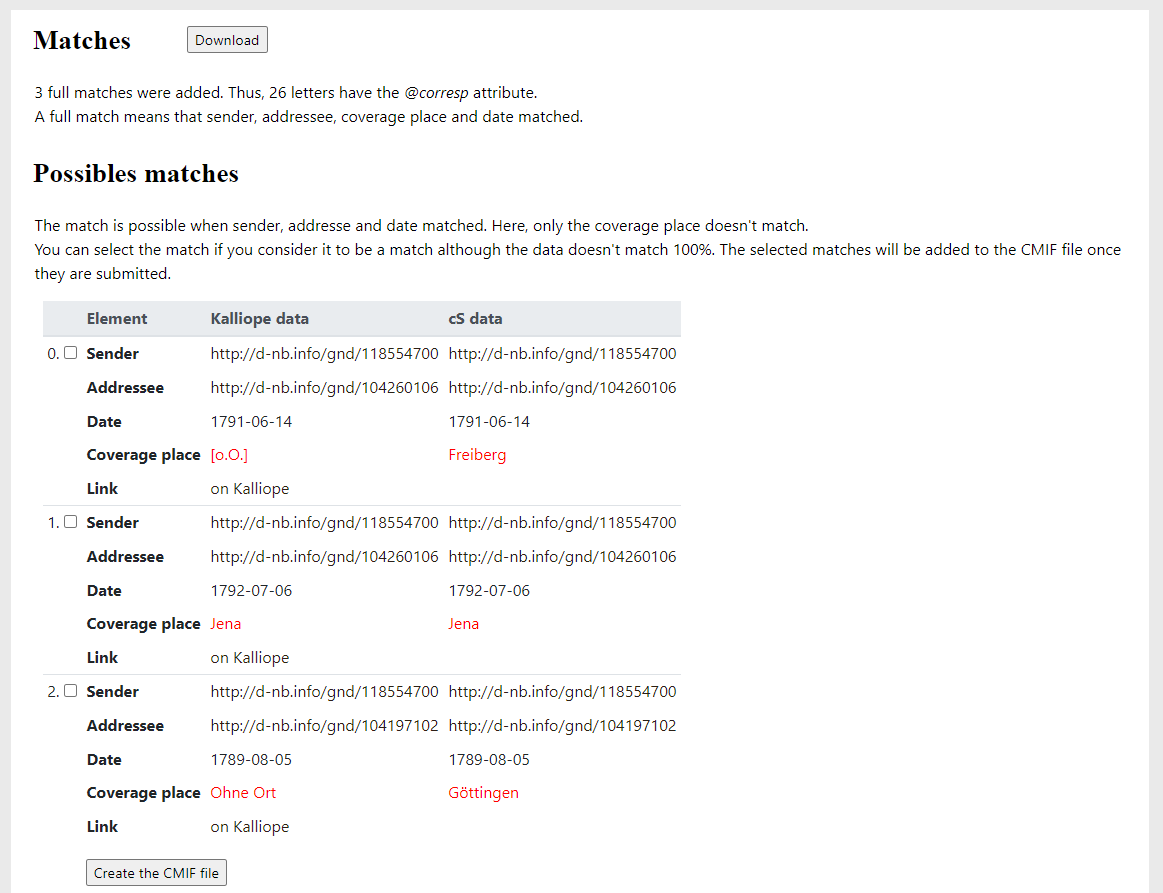
\includegraphics[width=15cm]{img/csMT_possiblematches.png}
         \caption{Page \textit{possibles matches} du cS matching tool}
         \vspace{-10pt}
\end{figure}
Les matches à sélectionner se présentent sous forme de tableau. Pour chacun des matches, les données du Kalliope-Verbundkatalog apparaissent sur la gauche du tableau et sont mises en comparaison avec les données du fichier de l'utilisateur, positionnées à droite du tableau. Avec cet affichage, l'utilisateur peut comparer l'\gls{uri} vers la notice \gls{gnd} de l'expéditeur des deux fichiers ainsi que l'\gls{uri} vers la notice \gls{gnd} du destinataire, le lieu d'envoi et la date d'envoi. Les \gls{uri} du destinaire et de l'expéditeur sont cliquables. L'élément en rouge indique ce sur quoi le match ne s'est pas effectué. Le choix de cette couleur a pour but d'attirer l'attention de l'utilisateur. Un lien vers le document d'archive est également disponible c'est-à-dire vers le site du Kalliope-Verbundkatalog. L'utilisateur a ainsi directement accès au manuscrit et éventuellement à sa numérisation quand celle-ci est disponible. Il s'agit d'un élément supplémentaire afin d'aider l'utilisateur dans la corrélation et la reconnaissance d'une lettre. Il peut ensuite sélectionner les lettres qui ont trouvé leur bonne corrélation grâce à une petite case disponible à côté du numéro de ligne du tableau. Une fois tous les matches passés en revue, une soumission des sélections est requise afin d'ajouter les liens du Kalliope-Verbundkatalog des lettres correspondances au sein du fichier \gls{cmif}. 

À cette étape, l'utilisateur a également la possibilité de télécharger le fichier \gls{cmif} dans lequel les \textit{full matches} seulement ont déjà été ajoutés automatiquement par l'algorithme. Afin d'éclairer l'utilisateur, quelques lignes informatives sont jointes à cette étape et indiquent le nombre de lettres pour lesquelles un document d'archive était déjà renseigné (le nombre de lettre ayant un attribut \texttt{@corresp}) ainsi que le nombre de corrélations qui ont été ajoutées de manière automatique. Une fois les matches sélectionnés par l'utilisateur ont été soumis, ils sont ajoutés au fichier \gls{cmif} et l'utilisateur a la possibilité de télecharger deux fichiers différents :
\begin{itemize}
    \item un fichier \gls{cmif} contenant seulement les matches qu'ils soient complets ou bien qu'ils aient été ajoutés par l'utilisateur.
    \item le fichier \gls{cmif} déposé par l'utilisateur avec le lien vers le Kalliope-Verbundkatalog pour les lettres qui ont trouvé une corrélation. Ce document contient donc les lettres qui n'ont trouvé aucune correspondance et celles qui en ont trouvé une.
\end{itemize}
Ces fichiers sont téléchargeables et s'enregistrent directement sur l'ordinateur de l'utilisateur. 

\chapter{Apports et livrables}
Ce chapitre a pour but de mettre en perspective ce projet, de pointer du doigt ce qui mériterait d'être amélioré mais aussi d'exposer les perspectives de cet outil. Il est également intéressant de savoir ce que l'outil a apporté jusqu'alors et de quelle manière il a pu enrichir les données de correspSearch. Son accessibilité sera également abordée ainsi que les utilisateurs cibles. 

\section{Résultats et perspectives de l'outil développé}
\subsection{Enrichissement des données de correspSearch : les résultats}
Jusqu'alors, aucune lettre issue de la correspondance d'Alexander von Humboldt et stockée sur correspSearch ne possédait de lien vers son document d'archive. Grâce au cS matching tool, ces données ont pu être enrichies en ajoutant le lien correspondant vers le portail archivistique du Kalliope-Verbundkatalog. 

Au sein de correspSearch sont stockées 6193 lettres issues de la correspondance d'Alexander von Humboldt. Grâce à plusieurs ajustements dans le code, le nombre de matches complets a pu augmenter de 199 au premier lancement à 440 au dernier lancement de l'outil. Le nombre de matches possibles, c'est-à-dire un match pour lequel le lieu d'envoi n'est pas correspondant, a augmenté de 601 à 714. Suite au regard d'un utilisateur et après sa sélection, le nombre de lettres enregistrées sur correspSearch et pour lesquelles il a été possible d'ajouter le lien vers leur document d'archive s'élève au nombre de 705. Cela représente 11,3\% de la totalité des lettres enregistrées sur correspSearch issues de la correspondance d'Alexander von Humboldt. Est-ce beaucoup ou au contraire très peu ? Il est difficile de le dire et aucune estimation ou d'objectif à atteindre n'ont été évoqués avant le développement de cet outil. Il faut également préciser le fait que beaucoup de lettres n'ont pas des données complètes. Comme cela a été mentionné dans la définition des objectifs de cet outil \footnote{Voir \autoref{sect:objectifcSMT}}, beaucoup de lettres n'ont aucune indication concernant la date ou de lieu d'envoi. Quand un élément permettant corrélation entre les deux sets de données manque, il devient difficile de faire matcher deux lettres ensemble. Toutefois, l'efficacité de l'outil n'est pas seulement lié aux données et certaines parties de l'algorithme mériteraient d'être améliorées. 

\subsection{Améliorations et perspectives}
\subsubsection{Améliorations}
Certaines lettres ont été rédigées à plusieurs mains, cela signifie que plusieurs expéditeurs sont enregistrés dans les données. Toutefois, l'outil ne prend pas encore en compte les expéditeurs enregistrés sous forme de liste. L'algorithme fait donc correspondre toujours l'expéditeur enregistré en première position du document \gls{cmif} et des données issues du Kalliope-Verbundkatalog. Si la liste des expéditeurs n'est pas rangée de la même manière ou tout du moins le premier expéditeur enregistré n'est pas le même, l'algorithme ne détecte aucune corrélation possible. La fonction \texttt{matching()}, après améliorations, pourrait prendre en charge les listes d'expéditeurs et destinataires. Cela permettrait d'accroître le nombre de corrélations de lettres et d'enrichir par conséquent les données de correspSearch.

D'autre part, l'outil compare les identifiants \gls{gnd} du destinataire et de l'expéditeur des lettres. Faire correspondre les lettres sur des identifiants de notice d'autorité permet d'assurer plus facilement un match. Il serait également possible de faire correspondre les données sur la chaîne de caractère des noms et prénoms des destinataires et expéditeurs cependant nous ne sommes pas à l'abri des erreurs de typage ainsi que des diverses orthographes utilisées pour un seul et même nom. Faire correspondre les données sur l'identifiant \gls{gnd} s'accompagne également de désavantages. Certaines personnes ne possèdent aucun identifiant pérenne et ce pour plusieurs raisons : soit il s'agit d'un manque d'informations pour les identifier soit ils ne sont tout simplement pas enregistrés sur une base de bibliothèque et ne possèdent pas (encore) de notice d'autorité. Les lettres pour lesquelles le destinataire et/ou l'expéditeur n'ont pas d'identifiant ne pourront trouver corrélation. Sur le site internet de correspSearch\footnote{Voir la rubrique \textbf{ueber} sur le site de \href{https://correspsearch.net/de/ueber.html}{correspSearch}.}, il est indiqué que certaines personnes ne possède parfois pas d'identifiant \gls{gnd} enregistré et cela est complètement normal. La création d'une notice d'autorité prend du temps. Les bibliothèques n'ont pas beaucoup de temps à investir dans la création de nouvelles notices et une demande peut recevoir réponse plusieurs mois plus tard. Ainsi, si nous relançons l'outil dans quelques mois, certaines lettres qui n'ont pas trouvé corrélation actuellement trouveront peut-être à ce moment-ci.

\subsubsection{Perspectives}
CorrespSearch mentionne sur son site que les données issues des éditions numériques sont régulièrement actualisées de manière automatisée. Il serait judicieux d'insérer l'algorithme du cS matching tool lors de l'actualisation des données des éditions numériques vers correspSearch. Ainsi, les données de correspSearch seraient directement liées à leur manuscrit via le lien du Kalliope-Verbundkatalog lors de leur actualisation dans le portail des documents épistolaires sans avoir besoin de lancer l'outil développé. Cela rendrait la chaîne de mise à jour des données plus efficace car une étape, celle de l'enrichissement des données vers leur source archivistique, disparaîtrait. Les données seront ainsi mises à jour et par la même occasion enrichies. Il serait toutefois important de relancer de temps en temps le cS matching tool car les données du Kalliope-Verbundkatalog s'actualisent régulièrement et indépendamment de celles des éditions numériques. 

D'autre part, le cS matching tool prend en charge pour l'instant seulement la correspondance d'Alexander von Humboldt. En effet, l'utilisateur n'a pas la main sur les requêtes envoyées à l'\gls{api} du Kalliope-Verbundkatalog. Qu'importe si l'utilisateur dépose un fichier contenant des lettres de la correspondance d'une autre personne, la fonction enverra toujours deux requêtes pour récupérer les données de la correspondance de Humboldt. La fonction n'effectue d'ailleurs aucune vérification dans le document déposé par l'utilisateur afin de savoir si le fichier contient exclusivement des lettres issues de la correspondance d'Alexander von Humboldt. L'outil a été réalisé seulement pour répondre à un besoin très précis : l'enrichissement des données de correspSearch de la correspondance d'Alexander von Humboldt et non toutes les correspondances stockées sur le portail. Cela est dû au fait que mon stage s'est réalisé au sein du projet académique \textit{Alexander von Humboldt auf Reisen} et non dans le pôle des humanités numériques, \gls{telota}, qui touche à tous les projets scientifiques de la \gls{bbaw}. Toutefois et à l'avenir, il serait intéressant d'enrichir les capacités de l'outil et de développer l'enrichissement des données des échanges épistolaires d'autres personnages présents sur correspSearch. Pour cela, l'utilisateur pourrait par exemple indiquer l'identifiant \gls{gnd} de la personne pour laquelle il souhaiterait enrichir les données. Cet identifiant serait injecté au sein des requêtes envoyées à l'\gls{api} du Kalliope-Verbundkatalog permettant ainsi de récupérer les données correspondantes. 


\section{Cible et accessibilité du projet}
Le cS matching tool a été développé avec l'idée d'enrichir les données de correspSearch et par conséquent d'être utilisé par un technicien de la \gls{bbaw} ou bien par un ou une stagiaire. Dans tous les cas, il n'a pas à vocation d'être grand public. Toutefois, l'expérience utilisateur est suffisamment simple afin que la personne qui doit réaliser cette tâche puisse la faire de manière aisée. 

À présent et avec quelques améliorations du code et des fonctionnalités énoncées précédemment, l'outil pourrait être utile à tous les projets d'éditions numériques de documents épistolaires dont les données sont stockées en \gls{cmif}. Ces projets d'éditions numériques pourraient utiliser l'outil afin d'enrichir leurs propres données en ajoutant un lien vers le Kalliope-Verbundkatalog. Bien entendu, l'enrichissement a lieu seulement si l'outil trouve une corrélation et/ou que l'utilisateur en a sélectionné. 

En attendant que ces fonctionnalités soient implémentées, le projet est entièrement disponible en \textit{open source}. Il est hébergé sur la plateforme GitHub\footnote{Voir le projet \href{https://github.com/edition-humboldt-collection/cS-matchingtool}{sur le dépôt GitHub.}} tout comme le projet qui a été mené précédemment à savoir l'exploration de la correspondance d'Alexander von Humboldt par des fonctions de recherche et des visualisations de données\footnote{Voir la partie \autoref{chap:accessibilités} sur les diverses accessibilités du projet.}.  \textit{Alexander von Humboldt auf Reisen} n'avait encore aucune plateforme permettant d'héberger les divers projets numériques qui étaient développés en son sein. L'outil chronotopographique\footnote{Voir \autoref{sect:chronotopographie}.} est quant à lui non disponible en \textit{open source} pour l'instant même si il a vocation de l'être dans le futur. Pour cela, l'équipe m'a demandé de créer une organisation GitHub qui héberge tous ces projets innovants en les centralisant en un seul et même endroit : \href{https://github.com/edition-humboldt-collection}{edition-humboldt-collection}. Cette organisation contient pour l'instant deux dépôts contenant les projets menés au cours de mon stage mais d'autres viendront s'ajouter à l'avenir. 


\chapter*{Conclusion}
\addcontentsline{toc}{chapter}{Conclusion}

Après un séjour à Paris, Alexander von Humboldt retourne le 6 décembre 1827 à Berlin et débute une série de lectures publiques sur la description physique de la Terre et de l'Univers. À la fin du mois de mars 1828, Humboldt a dispensé seize lectures\footnote{\cite{spies_resonance_2020}}. En proposant ses lectures de manière publique, Humboldt se positionne dans une éducation ouverte à tous et non plus exclusive à élite savante. Il indique, par cette prise de position novatrice, les découvertes des sciences naturelles émergentes comme appartenant à tous. Lors de ces conférences particulièrement appréciées du public, un nombre inhabituel de femmes y assistent. Depuis 1800, il revendique le fait de rendre accessible ses connaissances et ses publications au grand public. Humboldt apparaît comme un précurseur de la démocratisation et la vulgarisation du savoir. Ces conférences publiques ont débouché sur la rédaction de son oeuvre majeure, \textit{Cosmos}, publiée après 1845.

Le projet \textit{Alexander von Humboldt auf Reisen} se situe dans cette continuité, il contribue à rendre accessibles l'oeuvre et l'héritage manuscrit du scientifique. Afin d'atteindre cet objectif, les données produites par l'édition sont publiées dans des formats standards interopérables et accessibles sur le site internet qui lui est dédié\footnote{Voir le site \href{https://edition-humboldt.de/}{edition humboldt digital (ehd)}.}. L'importance de l'\textit{open data} et du \textit{linked data} ont été soulignés au cours de ce mémoire, mais il est nécessaire de rappeler que ces deux concepts sont primordiaux pour des projets de recherche comme celui-ci. En effet, en plus d'utiliser des données externes et d'enrichir de cette manière son corpus, publier des données ouvertes et liées insère l'édition au sein d'un large réseau et lui apporte une plus grande visibilité. La question de l'accessibilité aux données a été un thème transversal de ce mémoire et est parfaitement lié à l'\textit{open data}. Le souhait de Humboldt de rendre accessible à tous son héritage scientifique et manuscrit trouve écho dans le fait que les deux projets développés au cours de mon stage soient disponibles ouvertement sur la plateforme GitHub : \href{https://github.com/edition-humboldt-collection}{edition-humboldt-collection}. 

Ce mémoire s'est attaché à mettre en perspective le travail réalisé au cours du stage de quatre mois que j'ai effectué au sein de l'équipe de ce projet. Les missions qui m'ont été confiées consistaient à l'élaboration de fonctions de recherche et de visualisations de la correspondance d'Alexander von Humboldt d'une part et au développement d'un outil de corrélation dans le but d'enrichir les données de la correspondance du scientifique issues de correspSearch d'autre part. Mes réalisations se sont attachées à fournir des solutions à chaque étape de la conception de ces deux missions qui ont évolué au fur et à mesure en s'adaptant aux attentes de l'équipe de recherche.

Maintenant que ces outils sont opérationnels, l'équipe de correspSearch disposent à présent d'un outil de corrélation permettant d'enrichir les données de la correspondance d'Alexander von Humboldt éditée et répertoriée dans sa base avec des données externes issues du Kalliope-Verbundkatalog. Ce projet, répondant à un besoin particulièrement précis, pourrait être élargi de façon à enrichir les données de toutes les correspondances de correspSearch. Plus largement et de manière plus ambitieuse, cet outil pourrait évoluer dans le but de proposer un enrichissement des données pour toutes les éditions numériques ayant des données encodées en \gls{cmif}. Les membres du projet \textit{Alexander von Humboldt auf Reisen} disposent, quant à eux, d'outils opérationnels répondant à des attentes définies en amont. L'exploration et la découverte de la correspondance d'Alexander von Humboldt à travers des fonctions de recherche bénéficieront dans un premier temps à l'équipe du projet académique et aux personnes extérieures ayant suffisamment de compétences techniques pour installer de manière autonome ces fonctions sur leur propre ordinateur. Ce projet a permis de prendre connaissance de l'ampleur de la correspondance de Humboldt pour ma part et de redécouvrir cette correspondance grâce à de nouvelles technologies pour les chercheurs. Un site web serait intéressant à développer afin que toute personne puisse avoir accès à ces données sans condition de compétences techniques préalables. Cela ferait également résonance à la volonté d'Humboldt énoncée dans les premières lignes de cette introduction. 

 

En fonction de la suite de ces outils, de l'envergure future à laquelle on les destine, du public cible et de la vocation de leur pérennisation, diverses évolutions et améliorations peuvent ainsi être envisagées et de nombreuses solutions aux problèmes soulevés pourront efficacement être mises en place. 


\part*{Bibliographies thématiques}
\addcontentsline{toc}{chapter}{Bibliographies thématiques}
\printbibliography[keyword={humanities},title={Sur les humanités numériques}]
\printbibliography[keyword={data},title={Sur les données et visualisations de données}]
\printbibliography[keyword={bbaw},title={Sur les projets de la BBAW}]
\printbibliography[keyword={humboldt},title={Sur Alexander von Humboldt}]



\printglossaries %par défaut cette commande produit un glossaire par type. 
%si on gère plusieurs glossaires et index, on aura peut-être besoin de glossaries-extra.
\listoffigures %les figures sont cliquables car paquet importé
\listoftables

\appendix %pour créer une partie annexe.
\part*{Annexes}
\addcontentsline{toc}{part}{Annexes}

\chapter{Le modèle de données en réseau de l'\textit{edition humboldt digital}}
\chaptermark{Le modèle de données en réseau}
\begin{figure}[h!]
    \centering
         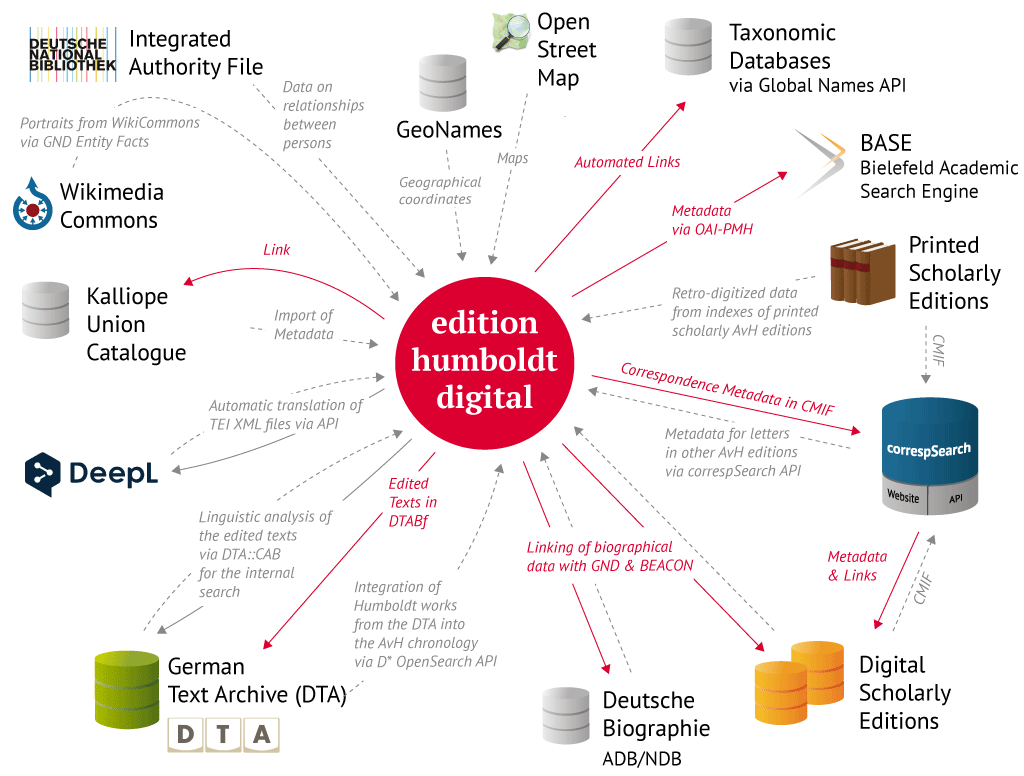
\includegraphics[angle=90,origin=c, height=13cm]{img/edition_humboldt_digital_v4_CC.png}
         \caption{Le modèle de donnnées en réseau de l'\textit{edition humboldt digital}}
         \label{fig:donneesReseau}
\end{figure}

\ChapterSub{Différence entre le format MODS et DC.}{Exemple d'une lettre de Abich envoyée à Humboldt en 1852 ou 1853.}
\chaptermark{Différence entre MODS et DC}
\label{annexe:MODSetDC}
\begin{figure}[h!]
    \centering
         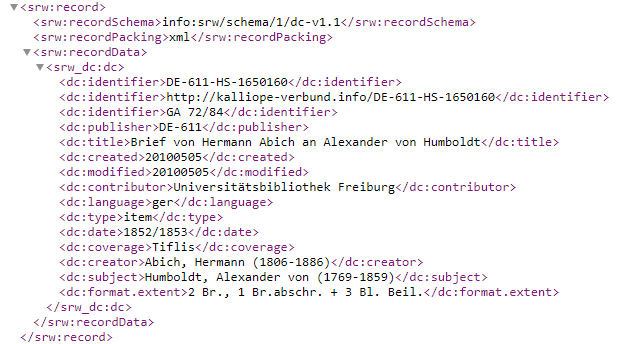
\includegraphics[width=16cm]{img/dc_letter_kalliope.png}
         \caption{Lettre encodée en format DC}
         \label{fig:DC}
\end{figure}
\begin{figure}[h!]
    \centering
         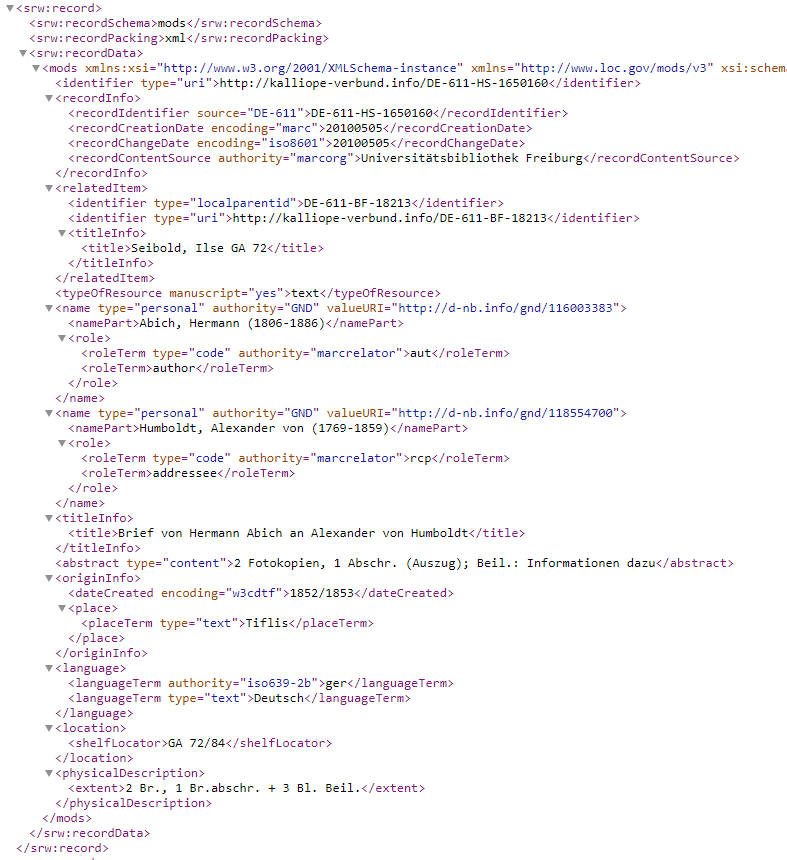
\includegraphics[width=16cm]{img/mods_kalliope.png}
         \caption{Lettre encodée en format MODS}
         \label{fig:MODS}
\end{figure}

\chapter{Fonction en Python retournant les informations géographiques d'un lieu donné}
\chaptermark{Fonction pour la géolocalisation}
\label{annexe:fGeolocalisation}

\begin{figure}[h]
\begin{lstlisting}
def get_geolocalisation_place(place):
    """
    Give the geolocation, geoname ID and ehd ID of a giving place.
    The function searches first in different local files :
    - placw register of edition humboldt
    - place register from GeoName
    If the place isn't already stored in one of this file, then
    a request is sent to the GeoName API.
    :param place: str
    :return: coverage_location
    :rtype: dict
    """
    ortsregister = getJSON('data/edh_ortsregister.json')
    or_geoname = getJSON('data/geoname_ortsregister.json')
    coverage_location = {}
    from_geoname = {}
    
    try :
        for o in ortsregister:
            # If the giving place is stored in the ehd place's register
            # then store infos in the dict coverage_location
            if place == o['properties']['ContentHeader'] :
                coverage_location["key"] = o['properties']['key']
                coverage_location['geoname_id'] = o['properties']['geoname_id']
                coverage_location['address'] = o['properties']['ContentHeader']
                coverage_location['coordinates'] = o['geometry']['coordinates']
    
        # If the giving place isn't in the ehd place's register then check
        # if it's stored in the geoname_ortsregister
        if bool(coverage_location)== False :
            for o in or_geoname:
                for i in o:
                    if place == o[i]["address"]:
                        coverage_location["key"] = o[i]['key']
                        coverage_location['geoname_id'] = o[i]['geoname_id']
                        coverage_location['address'] = i
                        coverage_location['coordinates'] = o[i]['coordinates']

        # If the giving place is neither in both local place's registers
        # then a request is sent to GeoName API      
        if bool(coverage_location)== False :
            location = geocoder.geonames(place, key='USER_KEY', featureClass='P')
            coverage_location['geoname_id'] = str(location.geonames_id)
            coverage_location['address'] = location.address
            coverage_location['coordinates'] = [location.lng, location.lat]
        
            for ort in ortsregister:
                if ort['properties']['geoname_id'] == str(coverage_location['geoname_id']):
                    coverage_location['key'] = ort['properties']['key']
            from_geoname[place] = coverage_location
        
        # If the geolocation from geoname wasn't already stored in the local
        # file, then they are added in it.
        if bool(from_geoname) == True:
            d = getJSON("data/geoname_ortsregister.json")
            d.append(from_geoname)            
            writeJSON("data/geoname_ortsregister.json", d)
    except :
        print(place)
    
    return coverage_location

\end{lstlisting}
\end{figure}



\ChapterSub{Aide à la recherche dactylographiée}{Exemples de pages tirées de l'aide à la recherche des archives Humboldt de la BBAW}
\chaptermark{Aide à la recherche dactylographie}

\begin{figure}[h!]
    \centering
         \includegraphics[width=15cm]{img/findbuch_ortsregister.jpg}
         \caption{Première page de l'index de lieux}
         \label{fig:findbuchOrtsregister}
\end{figure}

\begin{figure}[h!]
    \centering
    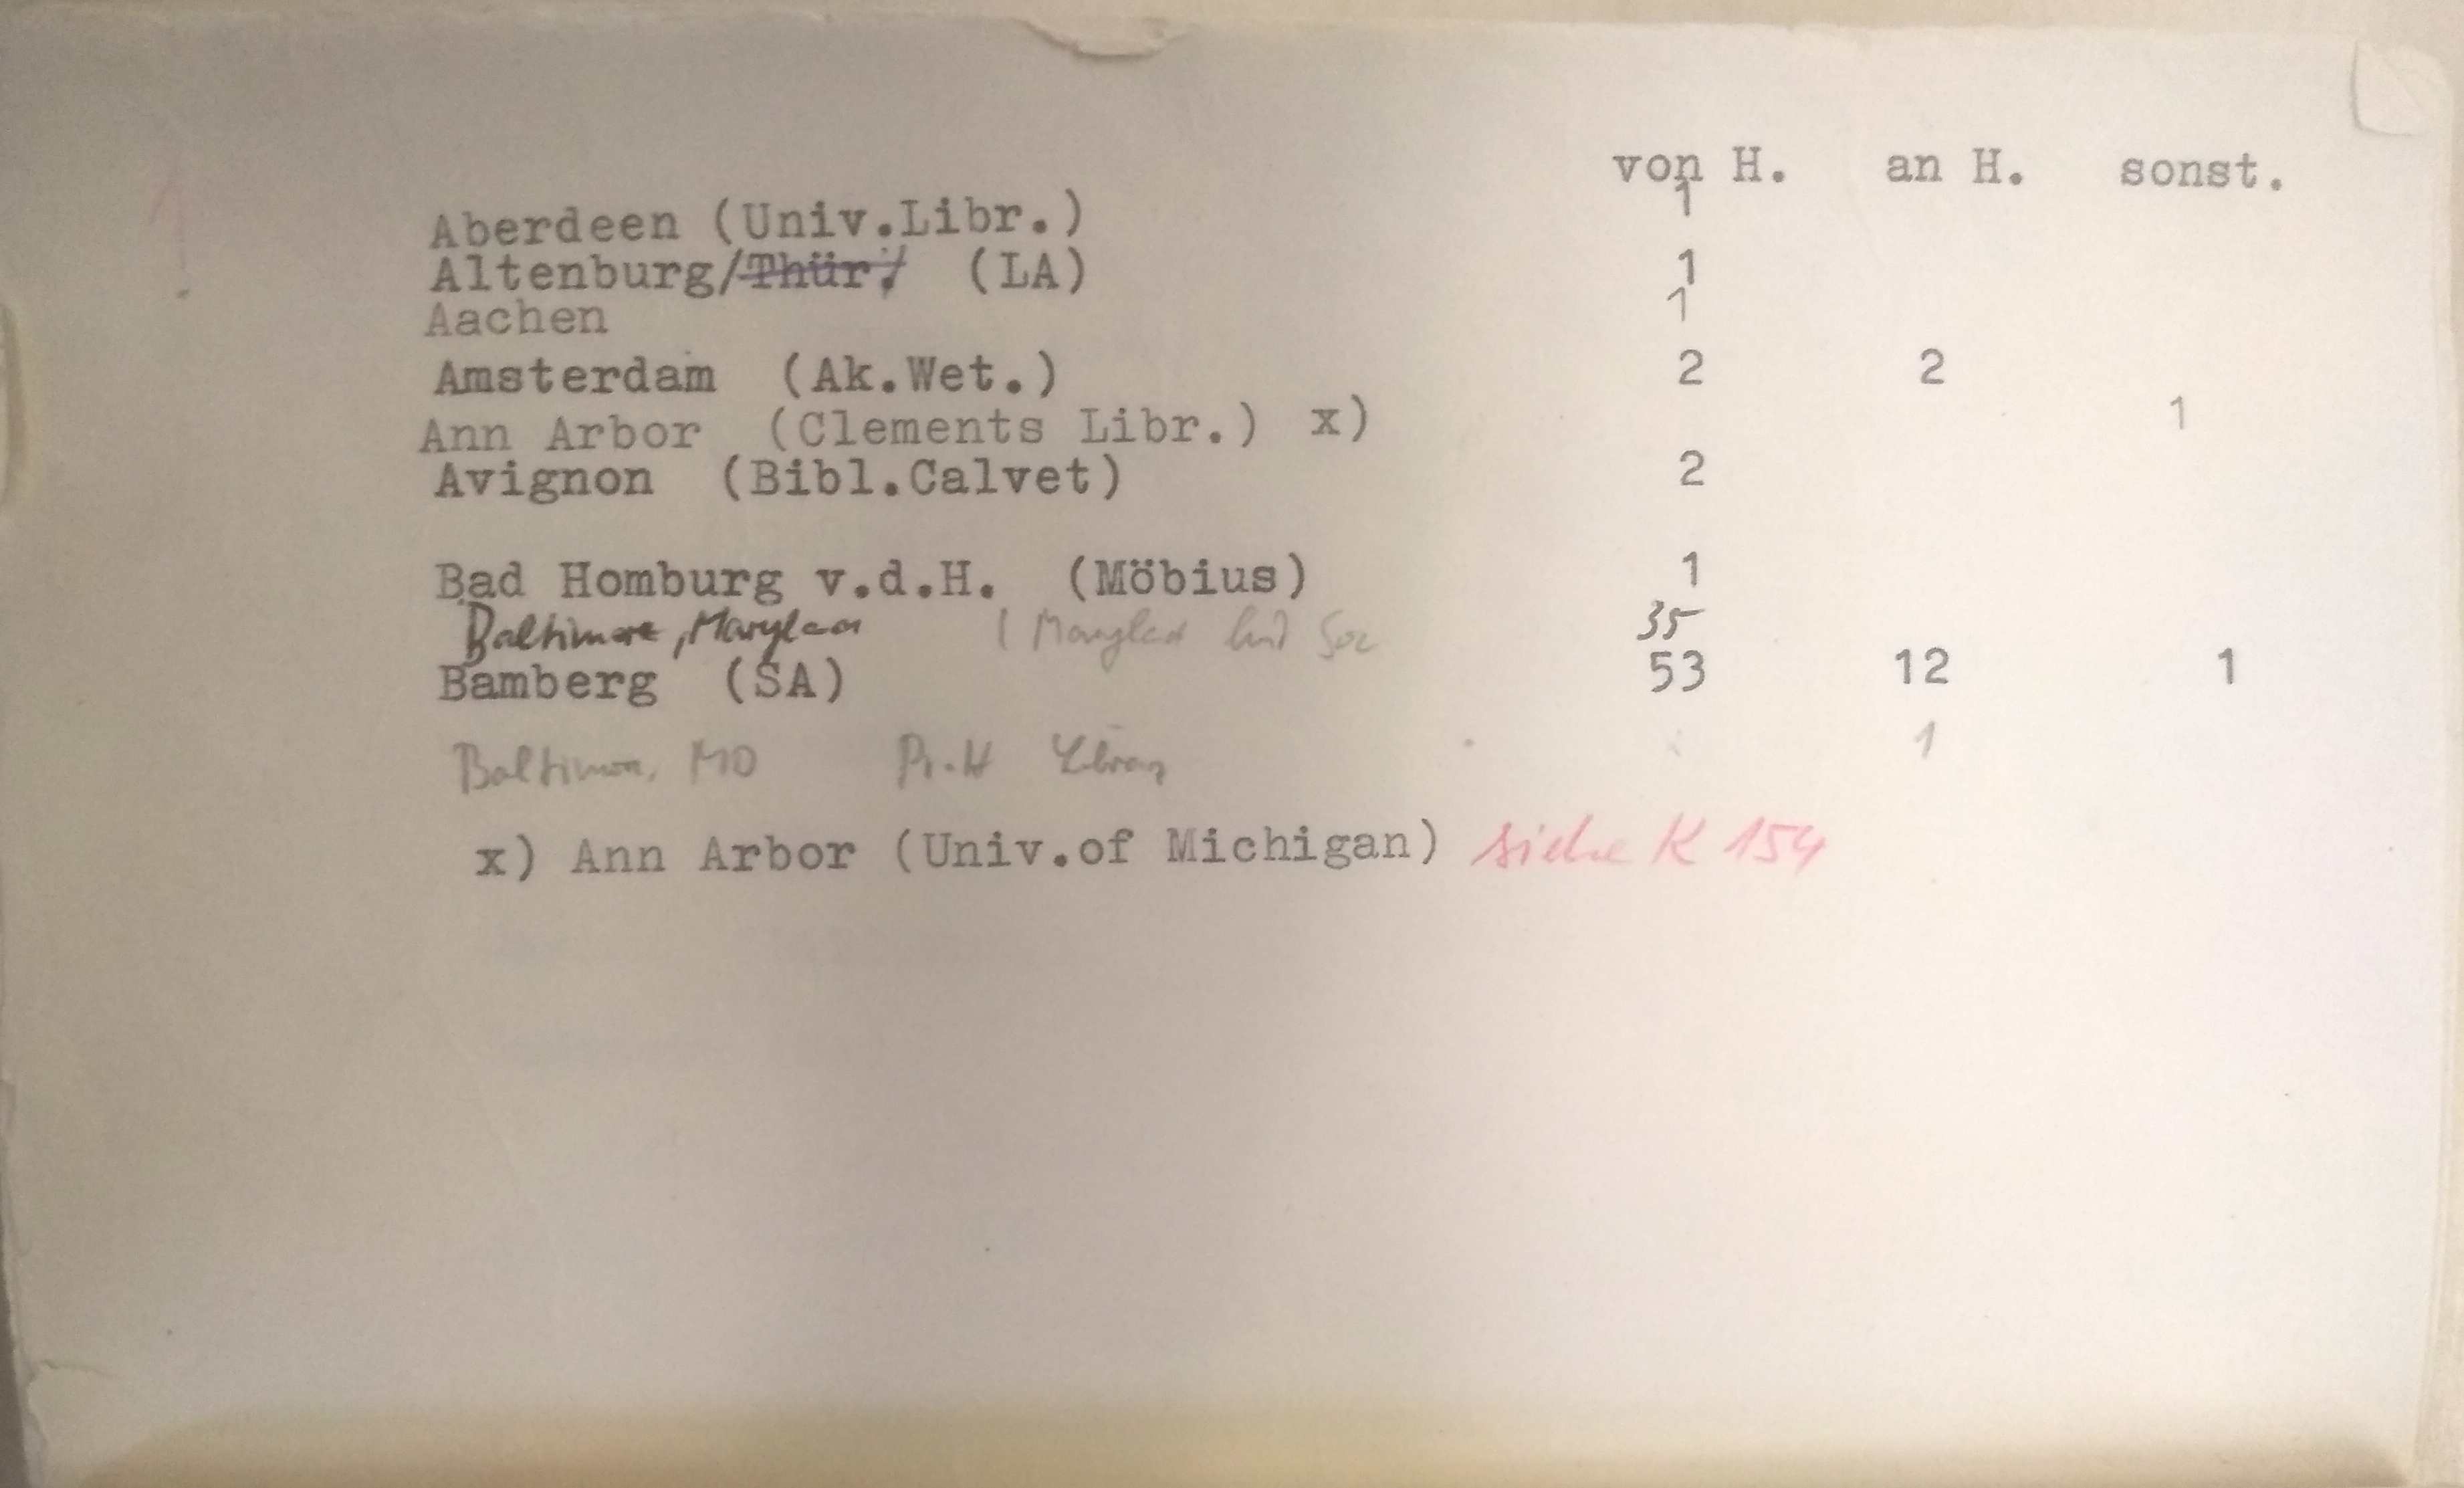
\includegraphics[width=15cm]{img/findbuch_detail.jpg}
    \caption{Détail des documents conservés pour les lieux de l'index}
    \label{fig:findbuchDocConserves}
\end{figure}


\ChapterSub{L'outil \textit{Humboldt Chronotopographie}}{Captures d'écran de l'outil expérimental}
\chaptermark{L'outil \textit{Humboldt Chronotographie}}
\begin{figure}[h!]
    \centering
    \caption{Visualisation des données extraites de l'aide à la recherche sur l'outil chronotopographique}
    \label{fig:chronoFindbuch}
    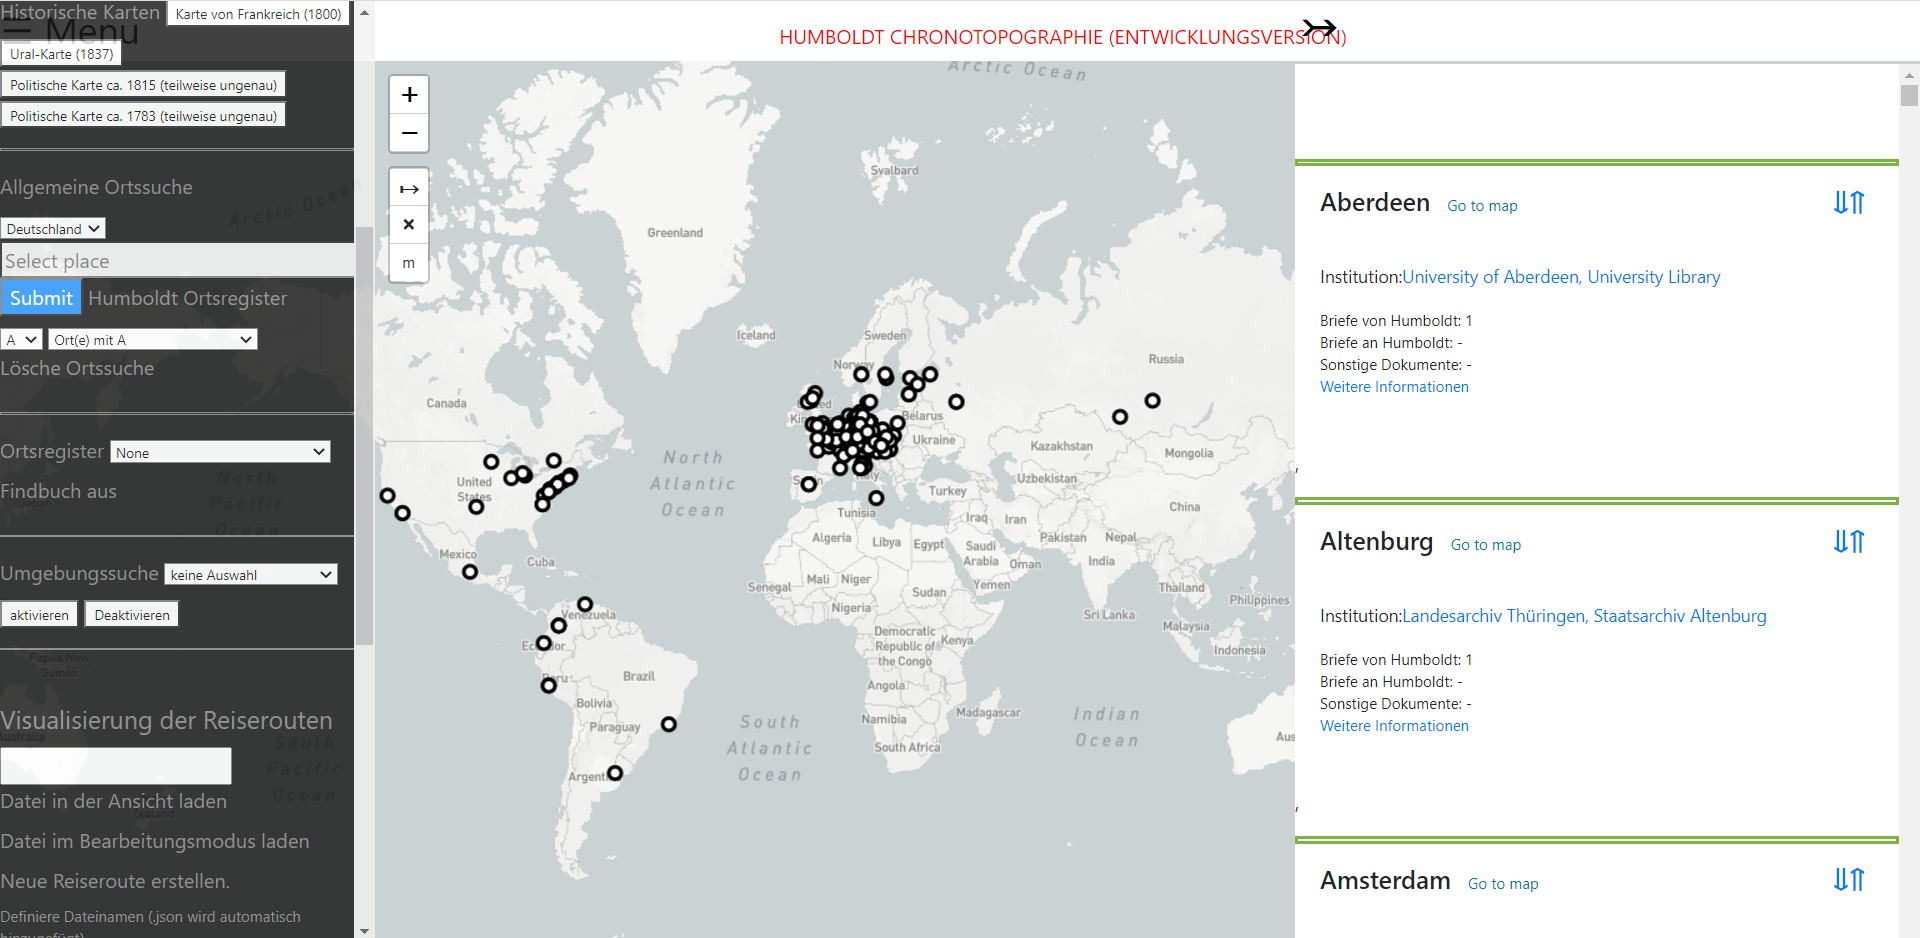
\includegraphics[angle=90,origin=c, height=17cm]{img/chronotopographie/chronoto_findbuch.png}
    \hfill
\end{figure}

\begin{figure}
    \centering
    \caption{Les différents fonds de cartes disponibles}
    \label{fig:fondsCartes}
    \begin{subfigure}[b]{0.8\textwidth}
        \centering
        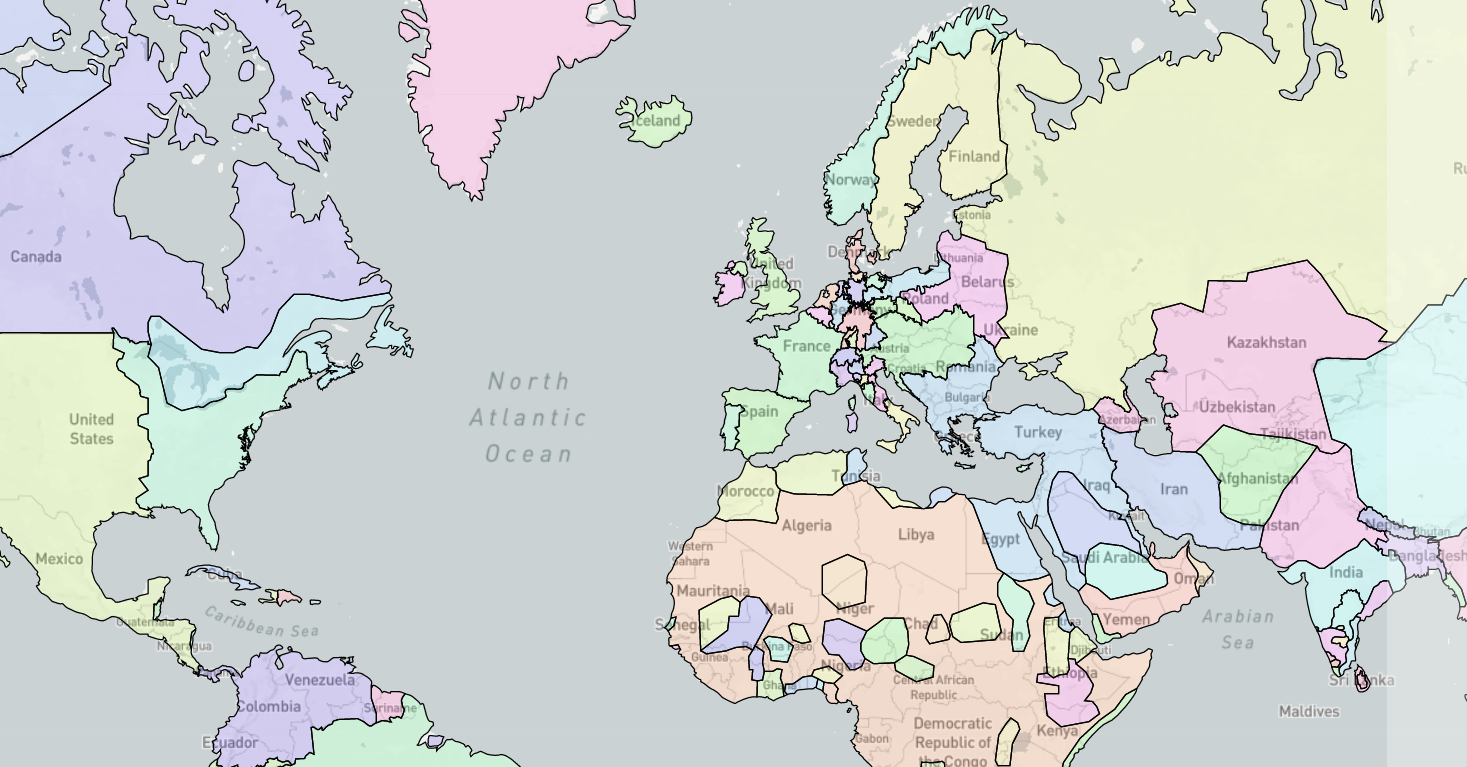
\includegraphics[width=1\linewidth]{img/chronotopographie/chrono_carte_1783.png}
        \caption{Fond de carte mondiale des frontières politiques vers 1783}
    \end{subfigure}
    \begin{subfigure}[b]{0.8\textwidth}
        \centering
        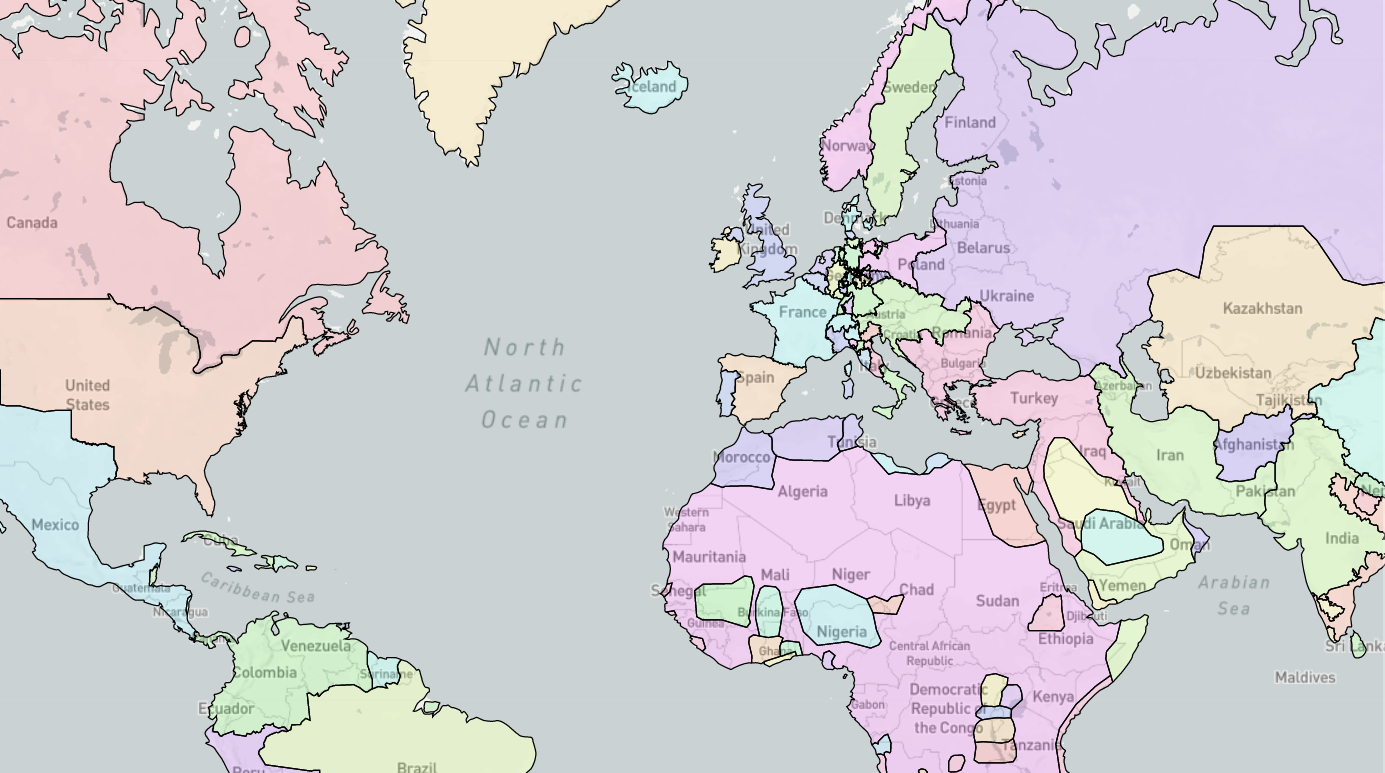
\includegraphics[width=1\linewidth]{img/chronotopographie/chrono_carte_1815.png}
        \caption{Fond de carte mondiale des frontières politiques vers 1815}
    \end{subfigure}
    \begin{subfigure}[b]{0.8\textwidth}
        \centering
        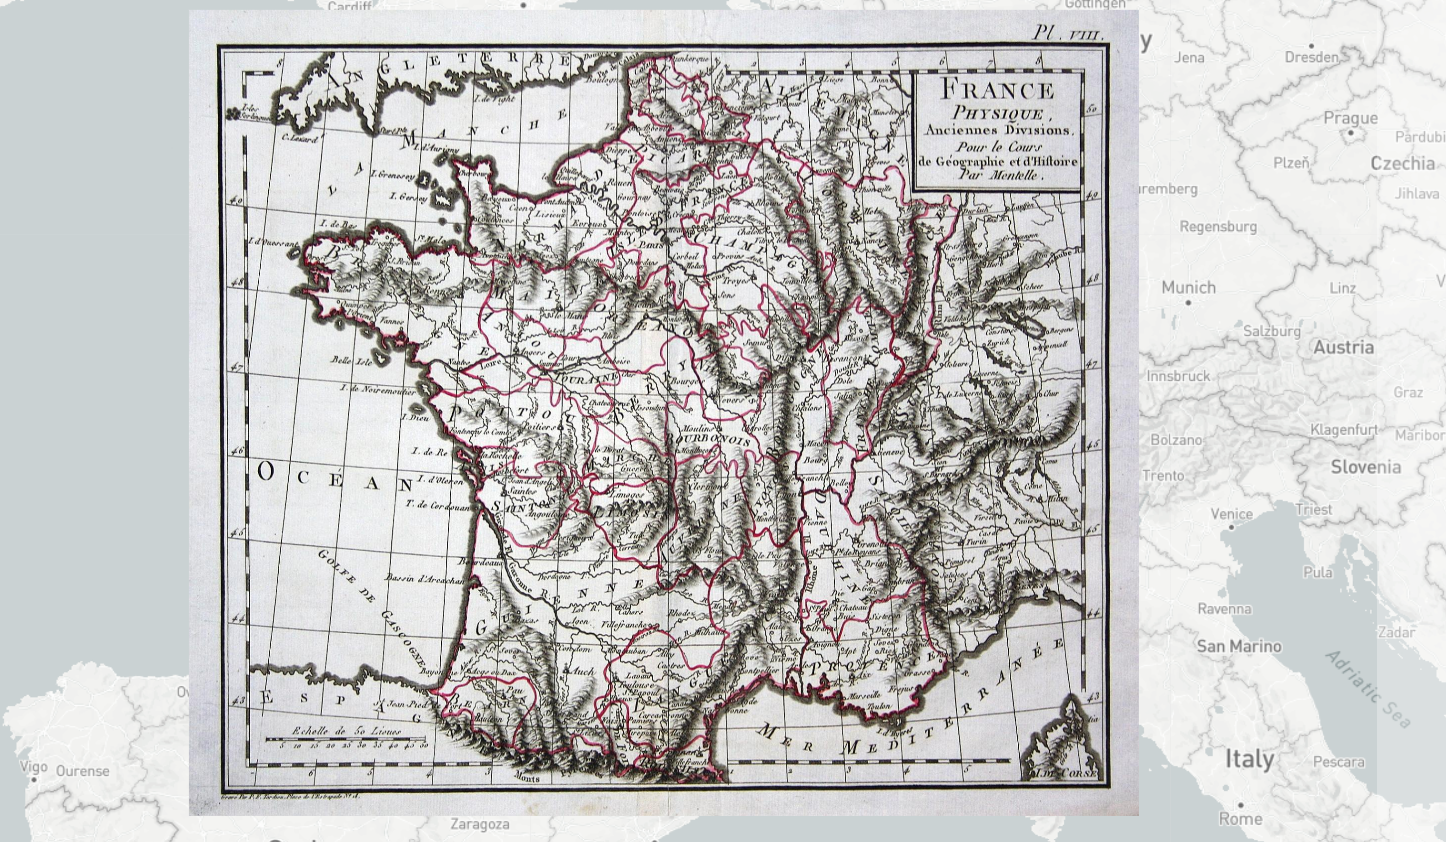
\includegraphics[width=1\linewidth]{img/chronotopographie/chrono_carte_france_1800.png}
        \caption{Fond de carte de la France vers 1800.}
    \end{subfigure}
    \vspace{-10pt}
\end{figure}

\chapter{Visualisations cartographiques}
\begin{changemargin}{-1cm}{-1cm}
\begin{figure}[h!]
\centering
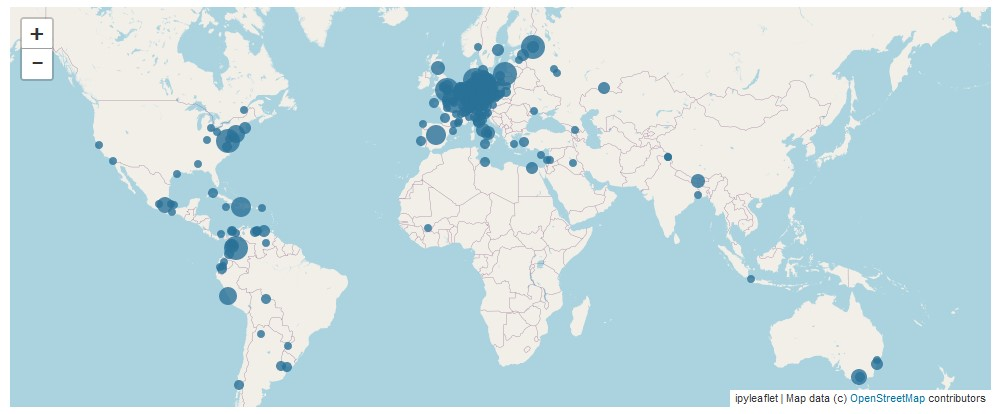
\includegraphics[scale=0.6]{img/mapviz_toutes.jpg}
\caption{Carte représentant toute la correspondance de Humboldt. La taille des points représentés est proportionnelle au nombre de lettres reçues ou envoyées.}
\label{fig:allLettersMap}
\end{figure}
\end{changemargin}

\begin{figure}[h!]
\centering
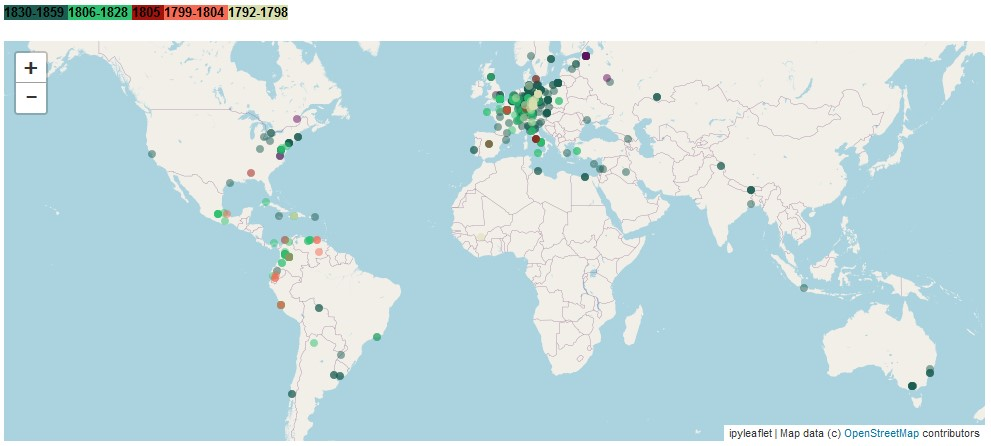
\includegraphics[angle=90,origin=c, height=15cm]{img/mapviz_color_legende.jpg}
\caption{Carte représentant toute la correspondance de Humboldt représentée sous six périodes différentes.}
\label{fig:allLettersMapColors}
\end{figure}

\chapter{Comparaison du design des sites web des projets de la BBAW}
\chaptermark{Design des sites de la BBAW}
\label{annexe:designBBAW}
\begin{figure}
    \centering
    
    \begin{subfigure}[b]{0.7\textwidth}
        \centering
        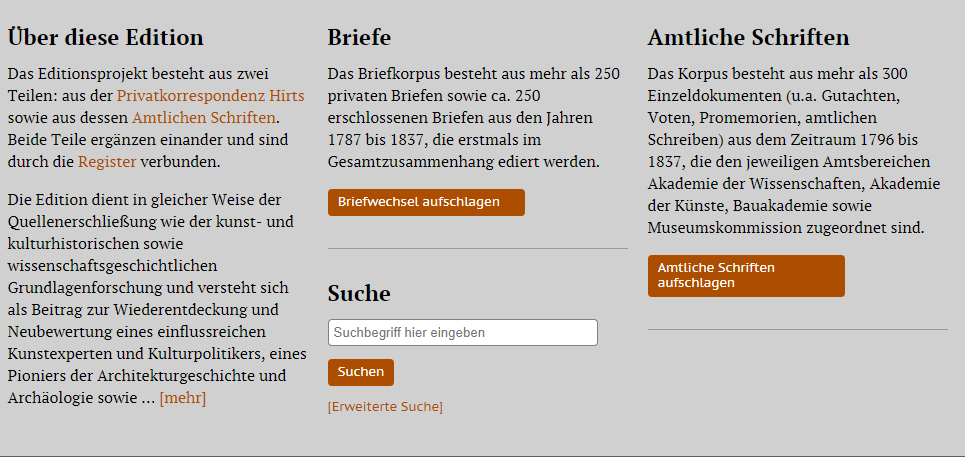
\includegraphics[width=1\linewidth]{img/aloys_websitepresentation.png}
        \caption{Extrait du \href{https://aloys-hirt.bbaw.de/}{site} de l'édition numérique des écrits et de la correspodance d'Aloys Hirt}
    \end{subfigure}
        \begin{subfigure}[b]{0.7\textwidth}
        \centering
        \includegraphics[width=1\linewidth]{img/iffland_websitepresentation.png}
        \caption{Extrait du \href{https://iffland.bbaw.de/}{site} de l'édition numérique des archives administratives et dramaturgiques d'August Iffland}
    \end{subfigure}
    \begin{subfigure}[b]{0.7\textwidth}
        \centering
        \includegraphics[width=1\linewidth]{img/ehd_websitepresentation.png}
        \caption{Extrait du \href{https://edition-humboldt.de/index.xql?l=en}{site} de l'édition numérique des carnets de voyages d'Alexander von Humboldt.}
    \end{subfigure}
    \vspace{-10pt}
\end{figure}

\newpage
\begin{figure}
    \centering
    \begin{subfigure}[b]{0.7\textwidth}
        \centering
        \includegraphics[width=1\linewidth]{img/corpusnummorum_websitepresentation.png}
        \caption{Extrait du \href{https://www.corpus-nummorum.eu/}{portail web} qui collecte et présente des données sur des monnaies provinciales romaines et grecques. }
    \end{subfigure}
        \begin{subfigure}[b]{0.7\textwidth}
        \centering
        \includegraphics[width=1\linewidth]{img/cS_websitepresentation.png}
        \caption{Extrait du \href{https://correspsearch.net/de/start.html}{site} de correspSearch}
    \end{subfigure}
    \begin{subfigure}[b]{0.7\textwidth}
        \centering
        \includegraphics[width=1\linewidth]{img/jeanpaul_websitepresentation.png}
        \caption{Extrait du \href{https://www.jeanpaul-edition.de/start.html}{site} de l'édition numérique de la correspondance de Jean Paul}
    \end{subfigure}
    \vspace{-10pt}
\end{figure}



\end{document}